
    \documentclass{article}
    \usepackage[top=2cm, bottom=2cm, outer=0.5cm, inner=0.5cm]{geometry}
    \usepackage[pages=some]{background}
    \usepackage{etoolbox}
    \usepackage{indentfirst}
    \AtBeginEnvironment{tabular}{\Large}
    \begin{document}
    

  \backgroundsetup{
    scale=1,
    color=black,
    opacity=0.2,
    angle=0,
    contents={%
        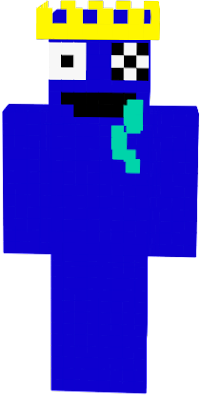
\includegraphics[width=\paperwidth,height=\paperheight]{../images/babao.png}
      }%
  }
  \BgThispage
  
  \begin{center}
    \huge
    Tabuada de Adição
  \end{center}

  \large
  \vspace{40pt}
  \noindent
  Registre o tempo gasto (em minutos):
  \begin{table}[!htpb]
    \begin{tabular}{|c|c|c|c|c|}
      \hline
      
    \begin{tabular}{ccccc}
1 & + & 2 & = & \\
    1 & + & 1 & = & \\
    1 & + & 7 & = & \\
    1 & + & 8 & = & \\
    1 & + & 4 & = & \\
    1 & + & 6 & = & \\
    1 & + & 3 & = & \\
    1 & + & 9 & = & \\
    1 & + & 5 & = & \\
    1 & + & 10 & = &
\end{tabular}&
    \begin{tabular}{ccccc}
2 & + & 6 & = & \\
    2 & + & 3 & = & \\
    2 & + & 5 & = & \\
    2 & + & 2 & = & \\
    2 & + & 4 & = & \\
    2 & + & 7 & = & \\
    2 & + & 9 & = & \\
    2 & + & 10 & = & \\
    2 & + & 8 & = & \\
    2 & + & 1 & = &
\end{tabular}&
    \begin{tabular}{ccccc}
3 & + & 3 & = & \\
    3 & + & 8 & = & \\
    3 & + & 2 & = & \\
    3 & + & 6 & = & \\
    3 & + & 5 & = & \\
    3 & + & 10 & = & \\
    3 & + & 9 & = & \\
    3 & + & 7 & = & \\
    3 & + & 1 & = & \\
    3 & + & 4 & = &
\end{tabular}&
    \begin{tabular}{ccccc}
4 & + & 10 & = & \\
    4 & + & 1 & = & \\
    4 & + & 5 & = & \\
    4 & + & 3 & = & \\
    4 & + & 8 & = & \\
    4 & + & 6 & = & \\
    4 & + & 7 & = & \\
    4 & + & 2 & = & \\
    4 & + & 4 & = & \\
    4 & + & 9 & = &
\end{tabular}&
    \begin{tabular}{ccccc}
5 & + & 10 & = & \\
    5 & + & 3 & = & \\
    5 & + & 8 & = & \\
    5 & + & 2 & = & \\
    5 & + & 1 & = & \\
    5 & + & 7 & = & \\
    5 & + & 4 & = & \\
    5 & + & 9 & = & \\
    5 & + & 5 & = & \\
    5 & + & 6 & = &
\end{tabular}
\\ \hline
    \begin{tabular}{ccccc}
6 & + & 2 & = & \\
    6 & + & 6 & = & \\
    6 & + & 8 & = & \\
    6 & + & 4 & = & \\
    6 & + & 9 & = & \\
    6 & + & 1 & = & \\
    6 & + & 7 & = & \\
    6 & + & 5 & = & \\
    6 & + & 3 & = & \\
    6 & + & 10 & = &
\end{tabular}&
    \begin{tabular}{ccccc}
7 & + & 8 & = & \\
    7 & + & 6 & = & \\
    7 & + & 4 & = & \\
    7 & + & 9 & = & \\
    7 & + & 10 & = & \\
    7 & + & 2 & = & \\
    7 & + & 3 & = & \\
    7 & + & 7 & = & \\
    7 & + & 5 & = & \\
    7 & + & 1 & = &
\end{tabular}&
    \begin{tabular}{ccccc}
8 & + & 9 & = & \\
    8 & + & 1 & = & \\
    8 & + & 3 & = & \\
    8 & + & 5 & = & \\
    8 & + & 2 & = & \\
    8 & + & 8 & = & \\
    8 & + & 4 & = & \\
    8 & + & 6 & = & \\
    8 & + & 10 & = & \\
    8 & + & 7 & = &
\end{tabular}&
    \begin{tabular}{ccccc}
9 & + & 7 & = & \\
    9 & + & 3 & = & \\
    9 & + & 1 & = & \\
    9 & + & 4 & = & \\
    9 & + & 9 & = & \\
    9 & + & 5 & = & \\
    9 & + & 10 & = & \\
    9 & + & 2 & = & \\
    9 & + & 6 & = & \\
    9 & + & 8 & = &
\end{tabular}&
    \begin{tabular}{ccccc}
10 & + & 4 & = & \\
    10 & + & 3 & = & \\
    10 & + & 6 & = & \\
    10 & + & 7 & = & \\
    10 & + & 8 & = & \\
    10 & + & 2 & = & \\
    10 & + & 9 & = & \\
    10 & + & 1 & = & \\
    10 & + & 10 & = & \\
    10 & + & 5 & = &
\end{tabular}
      \\ \hline
    \end{tabular}
  \end{table}
  \vfil
  \begin{flushright}
    \begin{minipage}[b]{6cm}
      A tabuada é o objeto de estudo mais importante na Matemática. É o caminho para se chegar ao universo dos números. (José Carlos dos Santos)
    \end{minipage}
  \end{flushright}

  \newpage
  

  \backgroundsetup{
    scale=1,
    color=black,
    opacity=0.2,
    angle=0,
    contents={%
        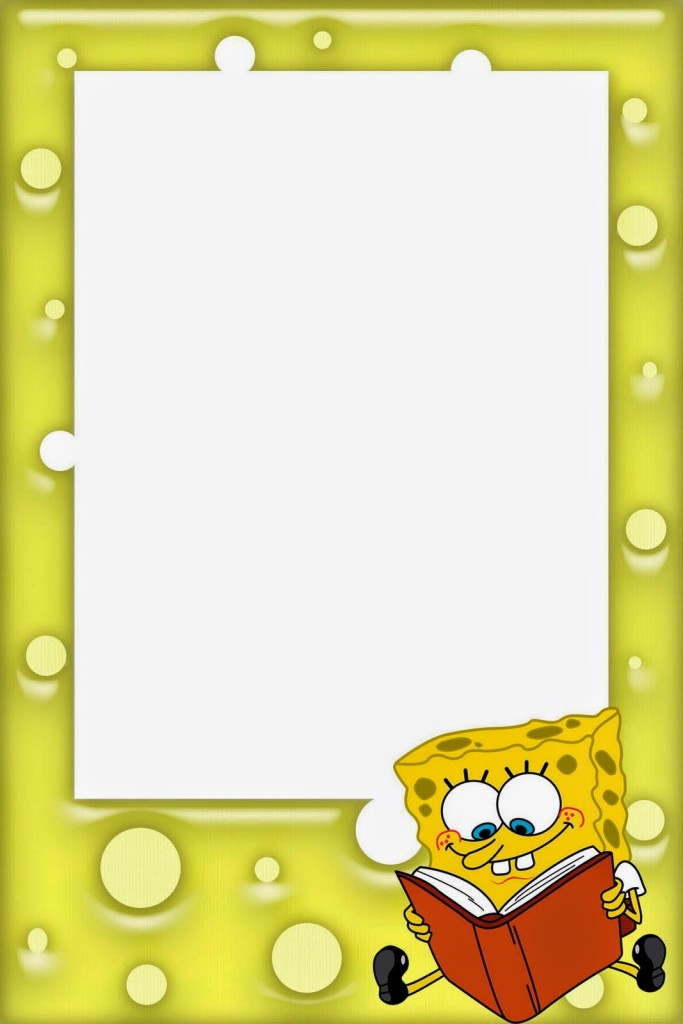
\includegraphics[width=\paperwidth,height=\paperheight]{../images/Bob-Esponja-estudando.jpg}
      }%
  }
  \BgThispage
  
  \begin{center}
    \huge
    Tabuada de Adição
  \end{center}

  \large
  \vspace{40pt}
  \noindent
  Registre o tempo gasto (em minutos):
  \begin{table}[!htpb]
    \begin{tabular}{|c|c|c|c|c|}
      \hline
      
    \begin{tabular}{ccccc}
1 & + & 1 & = & \\
    1 & + & 4 & = & \\
    1 & + & 10 & = & \\
    1 & + & 2 & = & \\
    1 & + & 7 & = & \\
    1 & + & 6 & = & \\
    1 & + & 3 & = & \\
    1 & + & 9 & = & \\
    1 & + & 8 & = & \\
    1 & + & 5 & = &
\end{tabular}&
    \begin{tabular}{ccccc}
2 & + & 5 & = & \\
    2 & + & 8 & = & \\
    2 & + & 2 & = & \\
    2 & + & 3 & = & \\
    2 & + & 10 & = & \\
    2 & + & 9 & = & \\
    2 & + & 6 & = & \\
    2 & + & 1 & = & \\
    2 & + & 4 & = & \\
    2 & + & 7 & = &
\end{tabular}&
    \begin{tabular}{ccccc}
3 & + & 9 & = & \\
    3 & + & 10 & = & \\
    3 & + & 6 & = & \\
    3 & + & 4 & = & \\
    3 & + & 1 & = & \\
    3 & + & 3 & = & \\
    3 & + & 2 & = & \\
    3 & + & 8 & = & \\
    3 & + & 7 & = & \\
    3 & + & 5 & = &
\end{tabular}&
    \begin{tabular}{ccccc}
4 & + & 2 & = & \\
    4 & + & 3 & = & \\
    4 & + & 10 & = & \\
    4 & + & 4 & = & \\
    4 & + & 6 & = & \\
    4 & + & 1 & = & \\
    4 & + & 5 & = & \\
    4 & + & 7 & = & \\
    4 & + & 8 & = & \\
    4 & + & 9 & = &
\end{tabular}&
    \begin{tabular}{ccccc}
5 & + & 7 & = & \\
    5 & + & 10 & = & \\
    5 & + & 9 & = & \\
    5 & + & 8 & = & \\
    5 & + & 6 & = & \\
    5 & + & 1 & = & \\
    5 & + & 3 & = & \\
    5 & + & 4 & = & \\
    5 & + & 5 & = & \\
    5 & + & 2 & = &
\end{tabular}
\\ \hline
    \begin{tabular}{ccccc}
6 & + & 10 & = & \\
    6 & + & 5 & = & \\
    6 & + & 9 & = & \\
    6 & + & 2 & = & \\
    6 & + & 4 & = & \\
    6 & + & 3 & = & \\
    6 & + & 8 & = & \\
    6 & + & 1 & = & \\
    6 & + & 6 & = & \\
    6 & + & 7 & = &
\end{tabular}&
    \begin{tabular}{ccccc}
7 & + & 2 & = & \\
    7 & + & 7 & = & \\
    7 & + & 1 & = & \\
    7 & + & 6 & = & \\
    7 & + & 4 & = & \\
    7 & + & 9 & = & \\
    7 & + & 5 & = & \\
    7 & + & 8 & = & \\
    7 & + & 10 & = & \\
    7 & + & 3 & = &
\end{tabular}&
    \begin{tabular}{ccccc}
8 & + & 2 & = & \\
    8 & + & 4 & = & \\
    8 & + & 6 & = & \\
    8 & + & 5 & = & \\
    8 & + & 7 & = & \\
    8 & + & 1 & = & \\
    8 & + & 10 & = & \\
    8 & + & 3 & = & \\
    8 & + & 9 & = & \\
    8 & + & 8 & = &
\end{tabular}&
    \begin{tabular}{ccccc}
9 & + & 2 & = & \\
    9 & + & 7 & = & \\
    9 & + & 3 & = & \\
    9 & + & 6 & = & \\
    9 & + & 10 & = & \\
    9 & + & 9 & = & \\
    9 & + & 4 & = & \\
    9 & + & 1 & = & \\
    9 & + & 8 & = & \\
    9 & + & 5 & = &
\end{tabular}&
    \begin{tabular}{ccccc}
10 & + & 9 & = & \\
    10 & + & 6 & = & \\
    10 & + & 7 & = & \\
    10 & + & 5 & = & \\
    10 & + & 3 & = & \\
    10 & + & 10 & = & \\
    10 & + & 4 & = & \\
    10 & + & 1 & = & \\
    10 & + & 2 & = & \\
    10 & + & 8 & = &
\end{tabular}
      \\ \hline
    \end{tabular}
  \end{table}
  \vfil
  \begin{flushright}
    \begin{minipage}[b]{6cm}
      A tabuada é o objeto de estudo mais importante na Matemática. É o caminho para se chegar ao universo dos números. (José Carlos dos Santos)
    \end{minipage}
  \end{flushright}

  \newpage
  

  \backgroundsetup{
    scale=1,
    color=black,
    opacity=0.2,
    angle=0,
    contents={%
        \includegraphics[width=\paperwidth,height=\paperheight]{../images/cute-galaxy-blue-frame-white-background-kids.jpg}
      }%
  }
  \BgThispage
  
  \begin{center}
    \huge
    Tabuada de Adição
  \end{center}

  \large
  \vspace{40pt}
  \noindent
  Registre o tempo gasto (em minutos):
  \begin{table}[!htpb]
    \begin{tabular}{|c|c|c|c|c|}
      \hline
      
    \begin{tabular}{ccccc}
1 & + & 5 & = & \\
    1 & + & 8 & = & \\
    1 & + & 1 & = & \\
    1 & + & 3 & = & \\
    1 & + & 4 & = & \\
    1 & + & 9 & = & \\
    1 & + & 6 & = & \\
    1 & + & 10 & = & \\
    1 & + & 2 & = & \\
    1 & + & 7 & = &
\end{tabular}&
    \begin{tabular}{ccccc}
2 & + & 4 & = & \\
    2 & + & 3 & = & \\
    2 & + & 2 & = & \\
    2 & + & 6 & = & \\
    2 & + & 7 & = & \\
    2 & + & 9 & = & \\
    2 & + & 8 & = & \\
    2 & + & 1 & = & \\
    2 & + & 10 & = & \\
    2 & + & 5 & = &
\end{tabular}&
    \begin{tabular}{ccccc}
3 & + & 9 & = & \\
    3 & + & 4 & = & \\
    3 & + & 1 & = & \\
    3 & + & 5 & = & \\
    3 & + & 2 & = & \\
    3 & + & 6 & = & \\
    3 & + & 7 & = & \\
    3 & + & 8 & = & \\
    3 & + & 3 & = & \\
    3 & + & 10 & = &
\end{tabular}&
    \begin{tabular}{ccccc}
4 & + & 4 & = & \\
    4 & + & 1 & = & \\
    4 & + & 6 & = & \\
    4 & + & 5 & = & \\
    4 & + & 3 & = & \\
    4 & + & 10 & = & \\
    4 & + & 2 & = & \\
    4 & + & 7 & = & \\
    4 & + & 9 & = & \\
    4 & + & 8 & = &
\end{tabular}&
    \begin{tabular}{ccccc}
5 & + & 7 & = & \\
    5 & + & 3 & = & \\
    5 & + & 4 & = & \\
    5 & + & 6 & = & \\
    5 & + & 10 & = & \\
    5 & + & 2 & = & \\
    5 & + & 9 & = & \\
    5 & + & 5 & = & \\
    5 & + & 1 & = & \\
    5 & + & 8 & = &
\end{tabular}
\\ \hline
    \begin{tabular}{ccccc}
6 & + & 6 & = & \\
    6 & + & 5 & = & \\
    6 & + & 8 & = & \\
    6 & + & 9 & = & \\
    6 & + & 4 & = & \\
    6 & + & 2 & = & \\
    6 & + & 1 & = & \\
    6 & + & 10 & = & \\
    6 & + & 7 & = & \\
    6 & + & 3 & = &
\end{tabular}&
    \begin{tabular}{ccccc}
7 & + & 6 & = & \\
    7 & + & 2 & = & \\
    7 & + & 9 & = & \\
    7 & + & 7 & = & \\
    7 & + & 3 & = & \\
    7 & + & 10 & = & \\
    7 & + & 4 & = & \\
    7 & + & 1 & = & \\
    7 & + & 8 & = & \\
    7 & + & 5 & = &
\end{tabular}&
    \begin{tabular}{ccccc}
8 & + & 6 & = & \\
    8 & + & 2 & = & \\
    8 & + & 9 & = & \\
    8 & + & 5 & = & \\
    8 & + & 10 & = & \\
    8 & + & 4 & = & \\
    8 & + & 7 & = & \\
    8 & + & 3 & = & \\
    8 & + & 1 & = & \\
    8 & + & 8 & = &
\end{tabular}&
    \begin{tabular}{ccccc}
9 & + & 5 & = & \\
    9 & + & 1 & = & \\
    9 & + & 7 & = & \\
    9 & + & 8 & = & \\
    9 & + & 4 & = & \\
    9 & + & 10 & = & \\
    9 & + & 3 & = & \\
    9 & + & 2 & = & \\
    9 & + & 6 & = & \\
    9 & + & 9 & = &
\end{tabular}&
    \begin{tabular}{ccccc}
10 & + & 4 & = & \\
    10 & + & 10 & = & \\
    10 & + & 6 & = & \\
    10 & + & 8 & = & \\
    10 & + & 5 & = & \\
    10 & + & 1 & = & \\
    10 & + & 7 & = & \\
    10 & + & 2 & = & \\
    10 & + & 9 & = & \\
    10 & + & 3 & = &
\end{tabular}
      \\ \hline
    \end{tabular}
  \end{table}
  \vfil
  \begin{flushright}
    \begin{minipage}[b]{6cm}
      A tabuada é o objeto de estudo mais importante na Matemática. É o caminho para se chegar ao universo dos números. (José Carlos dos Santos)
    \end{minipage}
  \end{flushright}

  \newpage
  

  \backgroundsetup{
    scale=1,
    color=black,
    opacity=0.2,
    angle=0,
    contents={%
        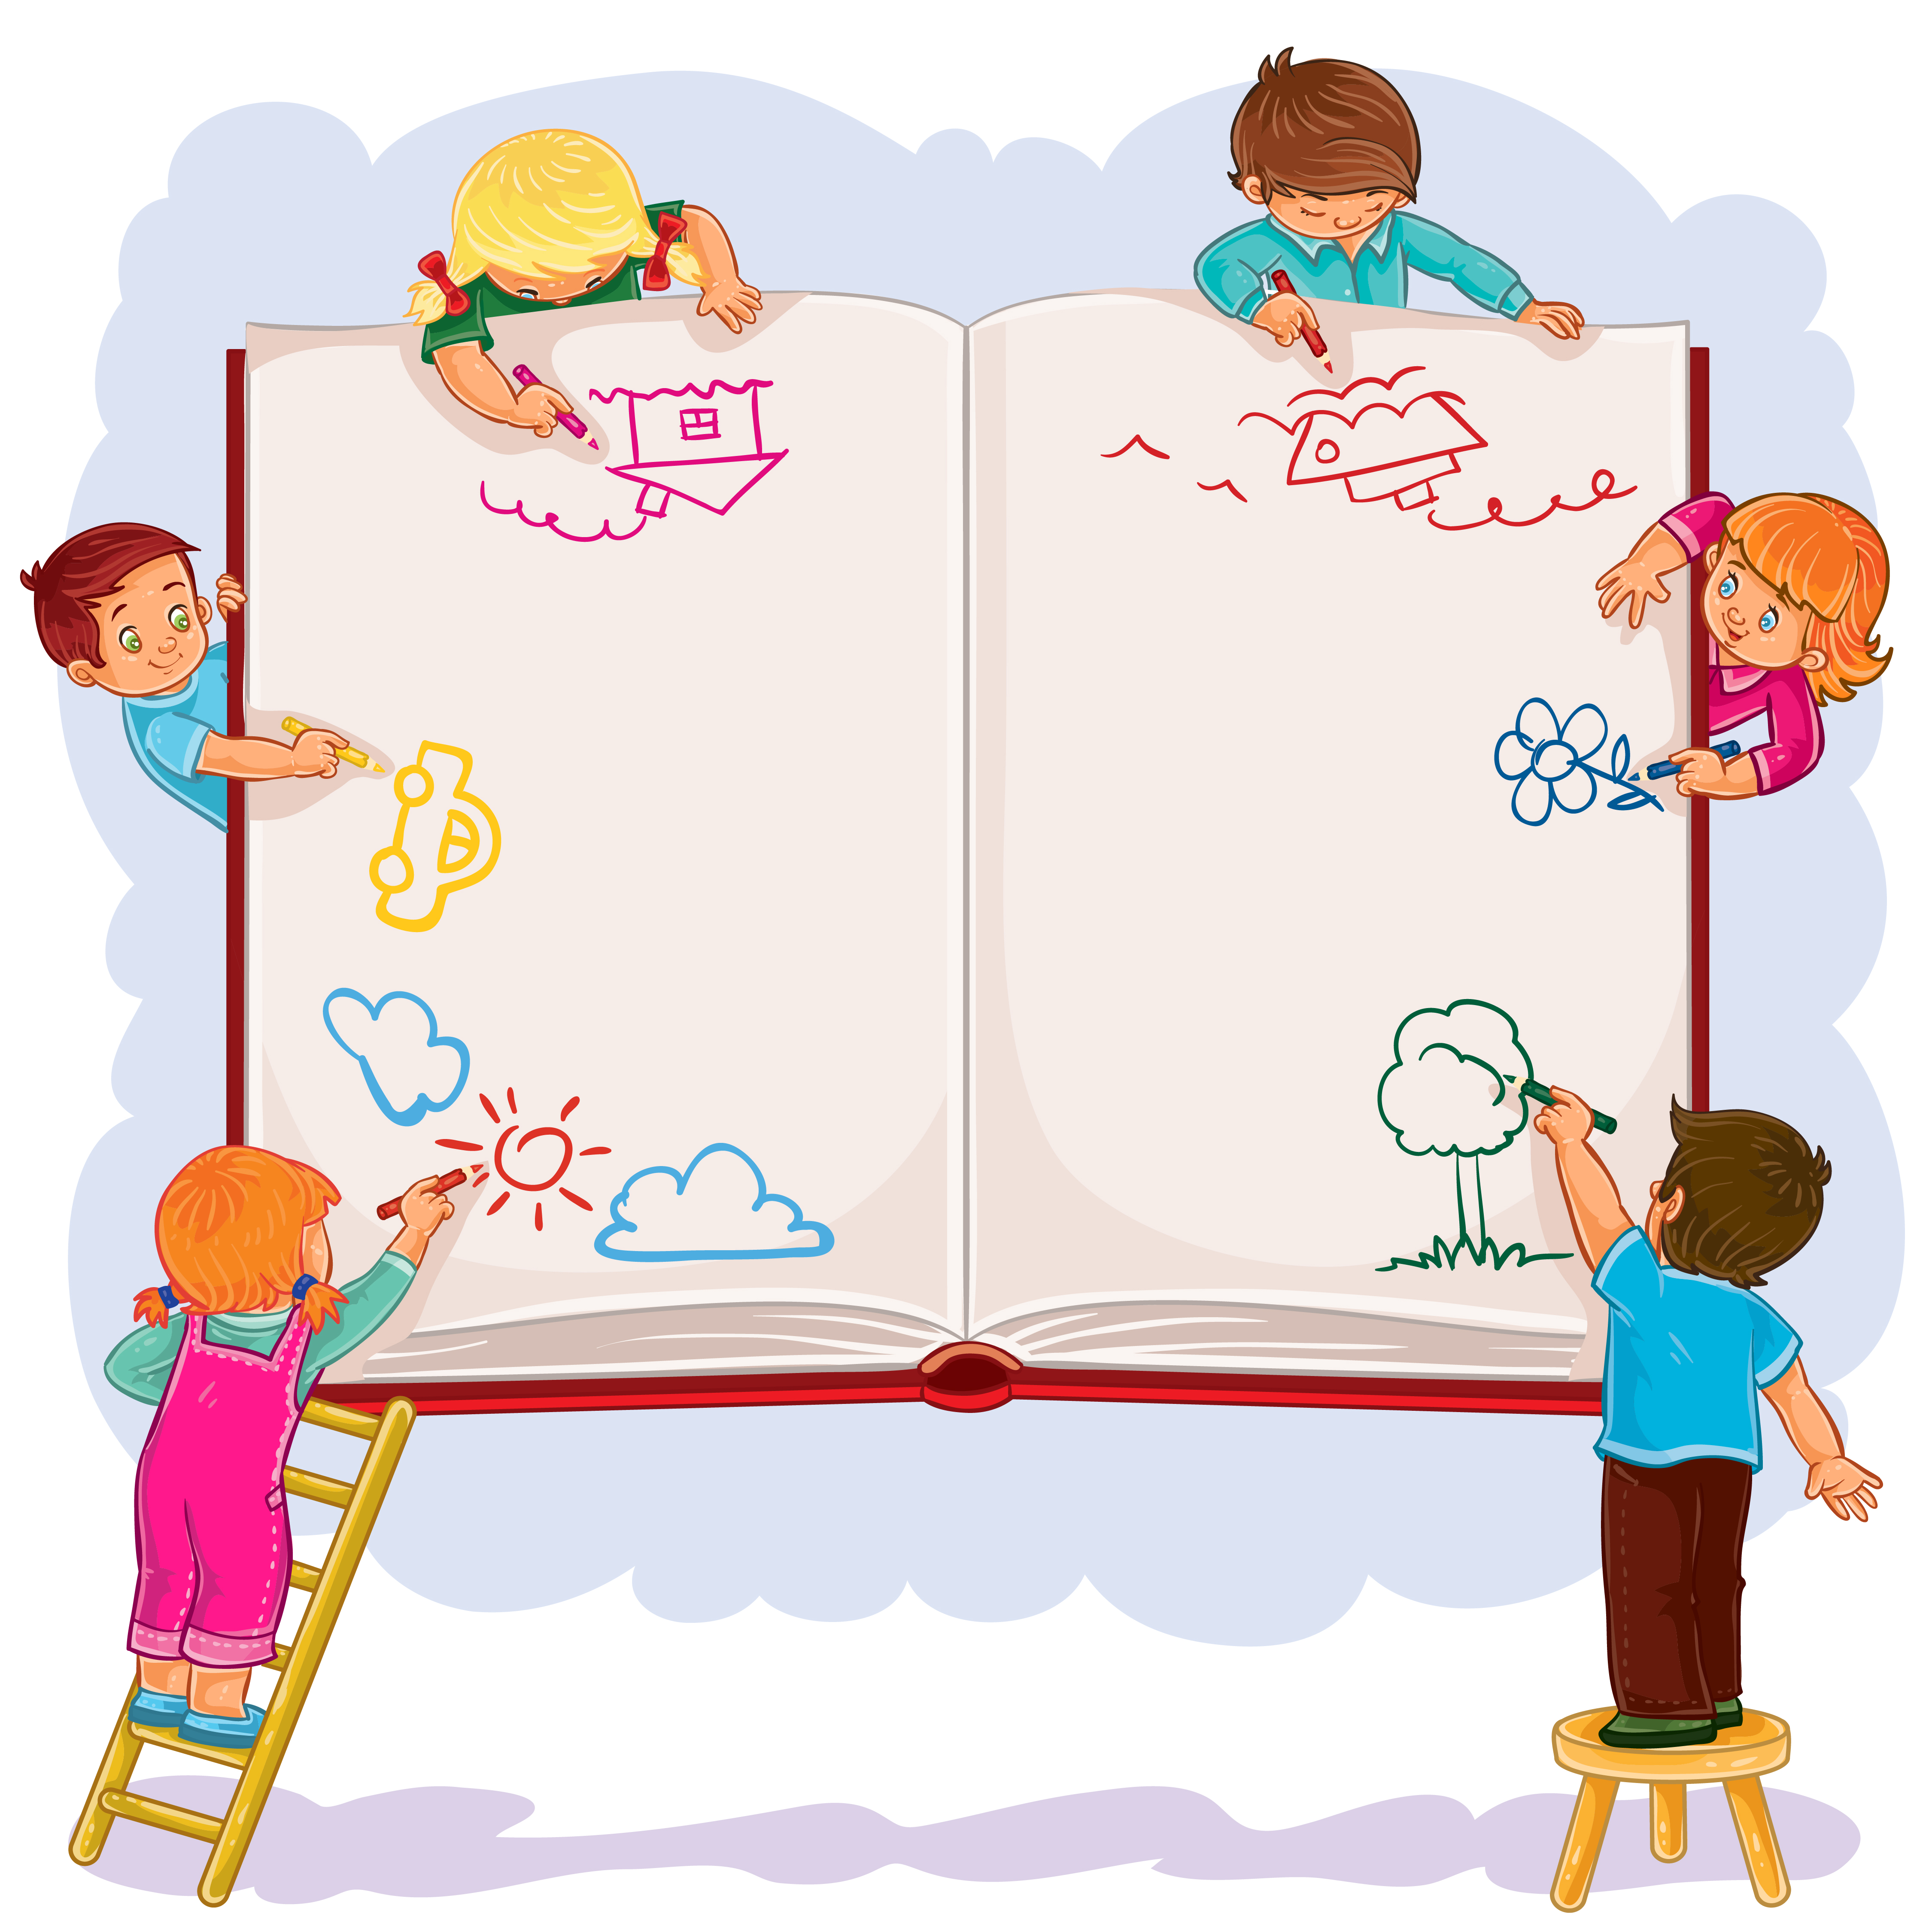
\includegraphics[width=\paperwidth,height=\paperheight]{../images/happy-children-together-draw-large-sheet-book.jpg}
      }%
  }
  \BgThispage
  
  \begin{center}
    \huge
    Tabuada de Adição
  \end{center}

  \large
  \vspace{40pt}
  \noindent
  Registre o tempo gasto (em minutos):
  \begin{table}[!htpb]
    \begin{tabular}{|c|c|c|c|c|}
      \hline
      
    \begin{tabular}{ccccc}
1 & + & 8 & = & \\
    1 & + & 5 & = & \\
    1 & + & 1 & = & \\
    1 & + & 7 & = & \\
    1 & + & 10 & = & \\
    1 & + & 2 & = & \\
    1 & + & 9 & = & \\
    1 & + & 6 & = & \\
    1 & + & 4 & = & \\
    1 & + & 3 & = &
\end{tabular}&
    \begin{tabular}{ccccc}
2 & + & 2 & = & \\
    2 & + & 1 & = & \\
    2 & + & 8 & = & \\
    2 & + & 5 & = & \\
    2 & + & 4 & = & \\
    2 & + & 3 & = & \\
    2 & + & 7 & = & \\
    2 & + & 9 & = & \\
    2 & + & 10 & = & \\
    2 & + & 6 & = &
\end{tabular}&
    \begin{tabular}{ccccc}
3 & + & 10 & = & \\
    3 & + & 2 & = & \\
    3 & + & 5 & = & \\
    3 & + & 8 & = & \\
    3 & + & 4 & = & \\
    3 & + & 6 & = & \\
    3 & + & 1 & = & \\
    3 & + & 9 & = & \\
    3 & + & 7 & = & \\
    3 & + & 3 & = &
\end{tabular}&
    \begin{tabular}{ccccc}
4 & + & 6 & = & \\
    4 & + & 2 & = & \\
    4 & + & 8 & = & \\
    4 & + & 5 & = & \\
    4 & + & 3 & = & \\
    4 & + & 10 & = & \\
    4 & + & 9 & = & \\
    4 & + & 7 & = & \\
    4 & + & 1 & = & \\
    4 & + & 4 & = &
\end{tabular}&
    \begin{tabular}{ccccc}
5 & + & 2 & = & \\
    5 & + & 1 & = & \\
    5 & + & 3 & = & \\
    5 & + & 4 & = & \\
    5 & + & 10 & = & \\
    5 & + & 5 & = & \\
    5 & + & 6 & = & \\
    5 & + & 9 & = & \\
    5 & + & 8 & = & \\
    5 & + & 7 & = &
\end{tabular}
\\ \hline
    \begin{tabular}{ccccc}
6 & + & 2 & = & \\
    6 & + & 5 & = & \\
    6 & + & 8 & = & \\
    6 & + & 10 & = & \\
    6 & + & 3 & = & \\
    6 & + & 7 & = & \\
    6 & + & 4 & = & \\
    6 & + & 6 & = & \\
    6 & + & 9 & = & \\
    6 & + & 1 & = &
\end{tabular}&
    \begin{tabular}{ccccc}
7 & + & 3 & = & \\
    7 & + & 7 & = & \\
    7 & + & 5 & = & \\
    7 & + & 4 & = & \\
    7 & + & 1 & = & \\
    7 & + & 6 & = & \\
    7 & + & 2 & = & \\
    7 & + & 9 & = & \\
    7 & + & 10 & = & \\
    7 & + & 8 & = &
\end{tabular}&
    \begin{tabular}{ccccc}
8 & + & 3 & = & \\
    8 & + & 8 & = & \\
    8 & + & 9 & = & \\
    8 & + & 5 & = & \\
    8 & + & 7 & = & \\
    8 & + & 10 & = & \\
    8 & + & 1 & = & \\
    8 & + & 4 & = & \\
    8 & + & 6 & = & \\
    8 & + & 2 & = &
\end{tabular}&
    \begin{tabular}{ccccc}
9 & + & 2 & = & \\
    9 & + & 7 & = & \\
    9 & + & 8 & = & \\
    9 & + & 5 & = & \\
    9 & + & 3 & = & \\
    9 & + & 10 & = & \\
    9 & + & 6 & = & \\
    9 & + & 1 & = & \\
    9 & + & 4 & = & \\
    9 & + & 9 & = &
\end{tabular}&
    \begin{tabular}{ccccc}
10 & + & 8 & = & \\
    10 & + & 5 & = & \\
    10 & + & 1 & = & \\
    10 & + & 7 & = & \\
    10 & + & 10 & = & \\
    10 & + & 3 & = & \\
    10 & + & 9 & = & \\
    10 & + & 2 & = & \\
    10 & + & 6 & = & \\
    10 & + & 4 & = &
\end{tabular}
      \\ \hline
    \end{tabular}
  \end{table}
  \vfil
  \begin{flushright}
    \begin{minipage}[b]{6cm}
      A tabuada é o objeto de estudo mais importante na Matemática. É o caminho para se chegar ao universo dos números. (José Carlos dos Santos)
    \end{minipage}
  \end{flushright}

  \newpage
  

  \backgroundsetup{
    scale=1,
    color=black,
    opacity=0.2,
    angle=0,
    contents={%
        \includegraphics[width=\paperwidth,height=\paperheight]{../images/jesus-children-white-background.jpg}
      }%
  }
  \BgThispage
  
  \begin{center}
    \huge
    Tabuada de Adição
  \end{center}

  \large
  \vspace{40pt}
  \noindent
  Registre o tempo gasto (em minutos):
  \begin{table}[!htpb]
    \begin{tabular}{|c|c|c|c|c|}
      \hline
      
    \begin{tabular}{ccccc}
1 & + & 5 & = & \\
    1 & + & 3 & = & \\
    1 & + & 2 & = & \\
    1 & + & 7 & = & \\
    1 & + & 8 & = & \\
    1 & + & 10 & = & \\
    1 & + & 9 & = & \\
    1 & + & 1 & = & \\
    1 & + & 6 & = & \\
    1 & + & 4 & = &
\end{tabular}&
    \begin{tabular}{ccccc}
2 & + & 5 & = & \\
    2 & + & 8 & = & \\
    2 & + & 2 & = & \\
    2 & + & 9 & = & \\
    2 & + & 7 & = & \\
    2 & + & 1 & = & \\
    2 & + & 10 & = & \\
    2 & + & 3 & = & \\
    2 & + & 6 & = & \\
    2 & + & 4 & = &
\end{tabular}&
    \begin{tabular}{ccccc}
3 & + & 7 & = & \\
    3 & + & 10 & = & \\
    3 & + & 1 & = & \\
    3 & + & 9 & = & \\
    3 & + & 6 & = & \\
    3 & + & 8 & = & \\
    3 & + & 3 & = & \\
    3 & + & 5 & = & \\
    3 & + & 2 & = & \\
    3 & + & 4 & = &
\end{tabular}&
    \begin{tabular}{ccccc}
4 & + & 10 & = & \\
    4 & + & 5 & = & \\
    4 & + & 7 & = & \\
    4 & + & 9 & = & \\
    4 & + & 4 & = & \\
    4 & + & 6 & = & \\
    4 & + & 3 & = & \\
    4 & + & 2 & = & \\
    4 & + & 1 & = & \\
    4 & + & 8 & = &
\end{tabular}&
    \begin{tabular}{ccccc}
5 & + & 10 & = & \\
    5 & + & 6 & = & \\
    5 & + & 9 & = & \\
    5 & + & 5 & = & \\
    5 & + & 3 & = & \\
    5 & + & 2 & = & \\
    5 & + & 7 & = & \\
    5 & + & 4 & = & \\
    5 & + & 1 & = & \\
    5 & + & 8 & = &
\end{tabular}
\\ \hline
    \begin{tabular}{ccccc}
6 & + & 7 & = & \\
    6 & + & 10 & = & \\
    6 & + & 5 & = & \\
    6 & + & 2 & = & \\
    6 & + & 1 & = & \\
    6 & + & 4 & = & \\
    6 & + & 6 & = & \\
    6 & + & 3 & = & \\
    6 & + & 8 & = & \\
    6 & + & 9 & = &
\end{tabular}&
    \begin{tabular}{ccccc}
7 & + & 1 & = & \\
    7 & + & 5 & = & \\
    7 & + & 10 & = & \\
    7 & + & 6 & = & \\
    7 & + & 8 & = & \\
    7 & + & 7 & = & \\
    7 & + & 4 & = & \\
    7 & + & 2 & = & \\
    7 & + & 3 & = & \\
    7 & + & 9 & = &
\end{tabular}&
    \begin{tabular}{ccccc}
8 & + & 8 & = & \\
    8 & + & 10 & = & \\
    8 & + & 2 & = & \\
    8 & + & 4 & = & \\
    8 & + & 9 & = & \\
    8 & + & 6 & = & \\
    8 & + & 3 & = & \\
    8 & + & 7 & = & \\
    8 & + & 1 & = & \\
    8 & + & 5 & = &
\end{tabular}&
    \begin{tabular}{ccccc}
9 & + & 5 & = & \\
    9 & + & 9 & = & \\
    9 & + & 3 & = & \\
    9 & + & 7 & = & \\
    9 & + & 8 & = & \\
    9 & + & 4 & = & \\
    9 & + & 10 & = & \\
    9 & + & 6 & = & \\
    9 & + & 2 & = & \\
    9 & + & 1 & = &
\end{tabular}&
    \begin{tabular}{ccccc}
10 & + & 1 & = & \\
    10 & + & 9 & = & \\
    10 & + & 6 & = & \\
    10 & + & 3 & = & \\
    10 & + & 4 & = & \\
    10 & + & 7 & = & \\
    10 & + & 8 & = & \\
    10 & + & 10 & = & \\
    10 & + & 2 & = & \\
    10 & + & 5 & = &
\end{tabular}
      \\ \hline
    \end{tabular}
  \end{table}
  \vfil
  \begin{flushright}
    \begin{minipage}[b]{6cm}
      A tabuada é o objeto de estudo mais importante na Matemática. É o caminho para se chegar ao universo dos números. (José Carlos dos Santos)
    \end{minipage}
  \end{flushright}

  \newpage
  

  \backgroundsetup{
    scale=1,
    color=black,
    opacity=0.2,
    angle=0,
    contents={%
        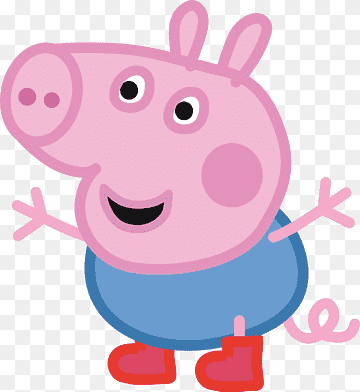
\includegraphics[width=\paperwidth,height=\paperheight]{../images/jorge.png}
      }%
  }
  \BgThispage
  
  \begin{center}
    \huge
    Tabuada de Adição
  \end{center}

  \large
  \vspace{40pt}
  \noindent
  Registre o tempo gasto (em minutos):
  \begin{table}[!htpb]
    \begin{tabular}{|c|c|c|c|c|}
      \hline
      
    \begin{tabular}{ccccc}
1 & + & 7 & = & \\
    1 & + & 9 & = & \\
    1 & + & 6 & = & \\
    1 & + & 10 & = & \\
    1 & + & 5 & = & \\
    1 & + & 4 & = & \\
    1 & + & 3 & = & \\
    1 & + & 8 & = & \\
    1 & + & 2 & = & \\
    1 & + & 1 & = &
\end{tabular}&
    \begin{tabular}{ccccc}
2 & + & 9 & = & \\
    2 & + & 8 & = & \\
    2 & + & 5 & = & \\
    2 & + & 1 & = & \\
    2 & + & 6 & = & \\
    2 & + & 7 & = & \\
    2 & + & 3 & = & \\
    2 & + & 10 & = & \\
    2 & + & 4 & = & \\
    2 & + & 2 & = &
\end{tabular}&
    \begin{tabular}{ccccc}
3 & + & 5 & = & \\
    3 & + & 2 & = & \\
    3 & + & 3 & = & \\
    3 & + & 10 & = & \\
    3 & + & 8 & = & \\
    3 & + & 4 & = & \\
    3 & + & 9 & = & \\
    3 & + & 1 & = & \\
    3 & + & 6 & = & \\
    3 & + & 7 & = &
\end{tabular}&
    \begin{tabular}{ccccc}
4 & + & 1 & = & \\
    4 & + & 5 & = & \\
    4 & + & 3 & = & \\
    4 & + & 6 & = & \\
    4 & + & 4 & = & \\
    4 & + & 9 & = & \\
    4 & + & 7 & = & \\
    4 & + & 8 & = & \\
    4 & + & 2 & = & \\
    4 & + & 10 & = &
\end{tabular}&
    \begin{tabular}{ccccc}
5 & + & 4 & = & \\
    5 & + & 1 & = & \\
    5 & + & 10 & = & \\
    5 & + & 5 & = & \\
    5 & + & 6 & = & \\
    5 & + & 7 & = & \\
    5 & + & 2 & = & \\
    5 & + & 3 & = & \\
    5 & + & 9 & = & \\
    5 & + & 8 & = &
\end{tabular}
\\ \hline
    \begin{tabular}{ccccc}
6 & + & 8 & = & \\
    6 & + & 5 & = & \\
    6 & + & 3 & = & \\
    6 & + & 6 & = & \\
    6 & + & 9 & = & \\
    6 & + & 4 & = & \\
    6 & + & 7 & = & \\
    6 & + & 2 & = & \\
    6 & + & 10 & = & \\
    6 & + & 1 & = &
\end{tabular}&
    \begin{tabular}{ccccc}
7 & + & 10 & = & \\
    7 & + & 8 & = & \\
    7 & + & 1 & = & \\
    7 & + & 5 & = & \\
    7 & + & 4 & = & \\
    7 & + & 2 & = & \\
    7 & + & 6 & = & \\
    7 & + & 7 & = & \\
    7 & + & 9 & = & \\
    7 & + & 3 & = &
\end{tabular}&
    \begin{tabular}{ccccc}
8 & + & 9 & = & \\
    8 & + & 7 & = & \\
    8 & + & 5 & = & \\
    8 & + & 10 & = & \\
    8 & + & 3 & = & \\
    8 & + & 1 & = & \\
    8 & + & 6 & = & \\
    8 & + & 8 & = & \\
    8 & + & 4 & = & \\
    8 & + & 2 & = &
\end{tabular}&
    \begin{tabular}{ccccc}
9 & + & 4 & = & \\
    9 & + & 1 & = & \\
    9 & + & 8 & = & \\
    9 & + & 9 & = & \\
    9 & + & 10 & = & \\
    9 & + & 6 & = & \\
    9 & + & 3 & = & \\
    9 & + & 2 & = & \\
    9 & + & 5 & = & \\
    9 & + & 7 & = &
\end{tabular}&
    \begin{tabular}{ccccc}
10 & + & 5 & = & \\
    10 & + & 1 & = & \\
    10 & + & 7 & = & \\
    10 & + & 9 & = & \\
    10 & + & 6 & = & \\
    10 & + & 3 & = & \\
    10 & + & 2 & = & \\
    10 & + & 4 & = & \\
    10 & + & 8 & = & \\
    10 & + & 10 & = &
\end{tabular}
      \\ \hline
    \end{tabular}
  \end{table}
  \vfil
  \begin{flushright}
    \begin{minipage}[b]{6cm}
      A tabuada é o objeto de estudo mais importante na Matemática. É o caminho para se chegar ao universo dos números. (José Carlos dos Santos)
    \end{minipage}
  \end{flushright}

  \newpage
  

  \backgroundsetup{
    scale=1,
    color=black,
    opacity=0.2,
    angle=0,
    contents={%
        
\includegraphics[width=\paperwidth,height=\paperheight]{../images/monkey-kings.jpg}
      }%
  }
  \BgThispage
  
  \begin{center}
    \huge
    Tabuada de Adição
  \end{center}

  \large
  \vspace{40pt}
  \noindent
  Registre o tempo gasto (em minutos):
  \begin{table}[!htpb]
    \begin{tabular}{|c|c|c|c|c|}
      \hline
      
    \begin{tabular}{ccccc}
1 & + & 3 & = & \\
    1 & + & 1 & = & \\
    1 & + & 7 & = & \\
    1 & + & 9 & = & \\
    1 & + & 10 & = & \\
    1 & + & 6 & = & \\
    1 & + & 8 & = & \\
    1 & + & 4 & = & \\
    1 & + & 5 & = & \\
    1 & + & 2 & = &
\end{tabular}&
    \begin{tabular}{ccccc}
2 & + & 2 & = & \\
    2 & + & 6 & = & \\
    2 & + & 8 & = & \\
    2 & + & 10 & = & \\
    2 & + & 1 & = & \\
    2 & + & 5 & = & \\
    2 & + & 3 & = & \\
    2 & + & 9 & = & \\
    2 & + & 7 & = & \\
    2 & + & 4 & = &
\end{tabular}&
    \begin{tabular}{ccccc}
3 & + & 4 & = & \\
    3 & + & 7 & = & \\
    3 & + & 5 & = & \\
    3 & + & 10 & = & \\
    3 & + & 3 & = & \\
    3 & + & 2 & = & \\
    3 & + & 8 & = & \\
    3 & + & 1 & = & \\
    3 & + & 6 & = & \\
    3 & + & 9 & = &
\end{tabular}&
    \begin{tabular}{ccccc}
4 & + & 5 & = & \\
    4 & + & 6 & = & \\
    4 & + & 8 & = & \\
    4 & + & 10 & = & \\
    4 & + & 4 & = & \\
    4 & + & 3 & = & \\
    4 & + & 7 & = & \\
    4 & + & 9 & = & \\
    4 & + & 1 & = & \\
    4 & + & 2 & = &
\end{tabular}&
    \begin{tabular}{ccccc}
5 & + & 5 & = & \\
    5 & + & 2 & = & \\
    5 & + & 8 & = & \\
    5 & + & 7 & = & \\
    5 & + & 9 & = & \\
    5 & + & 6 & = & \\
    5 & + & 1 & = & \\
    5 & + & 4 & = & \\
    5 & + & 3 & = & \\
    5 & + & 10 & = &
\end{tabular}
\\ \hline
    \begin{tabular}{ccccc}
6 & + & 10 & = & \\
    6 & + & 6 & = & \\
    6 & + & 9 & = & \\
    6 & + & 7 & = & \\
    6 & + & 2 & = & \\
    6 & + & 1 & = & \\
    6 & + & 4 & = & \\
    6 & + & 3 & = & \\
    6 & + & 8 & = & \\
    6 & + & 5 & = &
\end{tabular}&
    \begin{tabular}{ccccc}
7 & + & 3 & = & \\
    7 & + & 2 & = & \\
    7 & + & 10 & = & \\
    7 & + & 5 & = & \\
    7 & + & 1 & = & \\
    7 & + & 8 & = & \\
    7 & + & 6 & = & \\
    7 & + & 7 & = & \\
    7 & + & 9 & = & \\
    7 & + & 4 & = &
\end{tabular}&
    \begin{tabular}{ccccc}
8 & + & 6 & = & \\
    8 & + & 9 & = & \\
    8 & + & 3 & = & \\
    8 & + & 1 & = & \\
    8 & + & 2 & = & \\
    8 & + & 4 & = & \\
    8 & + & 7 & = & \\
    8 & + & 5 & = & \\
    8 & + & 10 & = & \\
    8 & + & 8 & = &
\end{tabular}&
    \begin{tabular}{ccccc}
9 & + & 8 & = & \\
    9 & + & 3 & = & \\
    9 & + & 2 & = & \\
    9 & + & 10 & = & \\
    9 & + & 5 & = & \\
    9 & + & 1 & = & \\
    9 & + & 4 & = & \\
    9 & + & 9 & = & \\
    9 & + & 6 & = & \\
    9 & + & 7 & = &
\end{tabular}&
    \begin{tabular}{ccccc}
10 & + & 10 & = & \\
    10 & + & 9 & = & \\
    10 & + & 5 & = & \\
    10 & + & 2 & = & \\
    10 & + & 4 & = & \\
    10 & + & 6 & = & \\
    10 & + & 1 & = & \\
    10 & + & 7 & = & \\
    10 & + & 3 & = & \\
    10 & + & 8 & = &
\end{tabular}
      \\ \hline
    \end{tabular}
  \end{table}
  \vfil
  \begin{flushright}
    \begin{minipage}[b]{6cm}
      A tabuada é o objeto de estudo mais importante na Matemática. É o caminho para se chegar ao universo dos números. (José Carlos dos Santos)
    \end{minipage}
  \end{flushright}

  \newpage
  

  \backgroundsetup{
    scale=1,
    color=black,
    opacity=0.2,
    angle=0,
    contents={%
        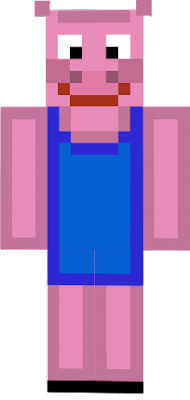
\includegraphics[width=\paperwidth,height=\paperheight]{../images/pepa.png}
      }%
  }
  \BgThispage
  
  \begin{center}
    \huge
    Tabuada de Adição
  \end{center}

  \large
  \vspace{40pt}
  \noindent
  Registre o tempo gasto (em minutos):
  \begin{table}[!htpb]
    \begin{tabular}{|c|c|c|c|c|}
      \hline
      
    \begin{tabular}{ccccc}
1 & + & 6 & = & \\
    1 & + & 10 & = & \\
    1 & + & 9 & = & \\
    1 & + & 2 & = & \\
    1 & + & 3 & = & \\
    1 & + & 1 & = & \\
    1 & + & 4 & = & \\
    1 & + & 8 & = & \\
    1 & + & 7 & = & \\
    1 & + & 5 & = &
\end{tabular}&
    \begin{tabular}{ccccc}
2 & + & 8 & = & \\
    2 & + & 5 & = & \\
    2 & + & 2 & = & \\
    2 & + & 6 & = & \\
    2 & + & 4 & = & \\
    2 & + & 3 & = & \\
    2 & + & 1 & = & \\
    2 & + & 7 & = & \\
    2 & + & 10 & = & \\
    2 & + & 9 & = &
\end{tabular}&
    \begin{tabular}{ccccc}
3 & + & 8 & = & \\
    3 & + & 7 & = & \\
    3 & + & 6 & = & \\
    3 & + & 2 & = & \\
    3 & + & 9 & = & \\
    3 & + & 5 & = & \\
    3 & + & 4 & = & \\
    3 & + & 10 & = & \\
    3 & + & 3 & = & \\
    3 & + & 1 & = &
\end{tabular}&
    \begin{tabular}{ccccc}
4 & + & 8 & = & \\
    4 & + & 10 & = & \\
    4 & + & 3 & = & \\
    4 & + & 9 & = & \\
    4 & + & 7 & = & \\
    4 & + & 4 & = & \\
    4 & + & 6 & = & \\
    4 & + & 5 & = & \\
    4 & + & 2 & = & \\
    4 & + & 1 & = &
\end{tabular}&
    \begin{tabular}{ccccc}
5 & + & 6 & = & \\
    5 & + & 2 & = & \\
    5 & + & 3 & = & \\
    5 & + & 5 & = & \\
    5 & + & 7 & = & \\
    5 & + & 10 & = & \\
    5 & + & 8 & = & \\
    5 & + & 4 & = & \\
    5 & + & 9 & = & \\
    5 & + & 1 & = &
\end{tabular}
\\ \hline
    \begin{tabular}{ccccc}
6 & + & 7 & = & \\
    6 & + & 4 & = & \\
    6 & + & 6 & = & \\
    6 & + & 3 & = & \\
    6 & + & 1 & = & \\
    6 & + & 10 & = & \\
    6 & + & 8 & = & \\
    6 & + & 5 & = & \\
    6 & + & 9 & = & \\
    6 & + & 2 & = &
\end{tabular}&
    \begin{tabular}{ccccc}
7 & + & 8 & = & \\
    7 & + & 5 & = & \\
    7 & + & 1 & = & \\
    7 & + & 3 & = & \\
    7 & + & 6 & = & \\
    7 & + & 10 & = & \\
    7 & + & 2 & = & \\
    7 & + & 9 & = & \\
    7 & + & 4 & = & \\
    7 & + & 7 & = &
\end{tabular}&
    \begin{tabular}{ccccc}
8 & + & 2 & = & \\
    8 & + & 1 & = & \\
    8 & + & 7 & = & \\
    8 & + & 3 & = & \\
    8 & + & 6 & = & \\
    8 & + & 5 & = & \\
    8 & + & 8 & = & \\
    8 & + & 10 & = & \\
    8 & + & 9 & = & \\
    8 & + & 4 & = &
\end{tabular}&
    \begin{tabular}{ccccc}
9 & + & 5 & = & \\
    9 & + & 3 & = & \\
    9 & + & 8 & = & \\
    9 & + & 6 & = & \\
    9 & + & 2 & = & \\
    9 & + & 1 & = & \\
    9 & + & 9 & = & \\
    9 & + & 10 & = & \\
    9 & + & 7 & = & \\
    9 & + & 4 & = &
\end{tabular}&
    \begin{tabular}{ccccc}
10 & + & 7 & = & \\
    10 & + & 9 & = & \\
    10 & + & 8 & = & \\
    10 & + & 5 & = & \\
    10 & + & 6 & = & \\
    10 & + & 4 & = & \\
    10 & + & 2 & = & \\
    10 & + & 1 & = & \\
    10 & + & 10 & = & \\
    10 & + & 3 & = &
\end{tabular}
      \\ \hline
    \end{tabular}
  \end{table}
  \vfil
  \begin{flushright}
    \begin{minipage}[b]{6cm}
      A tabuada é o objeto de estudo mais importante na Matemática. É o caminho para se chegar ao universo dos números. (José Carlos dos Santos)
    \end{minipage}
  \end{flushright}

  \newpage
  

  \backgroundsetup{
    scale=1,
    color=black,
    opacity=0.2,
    angle=0,
    contents={%
        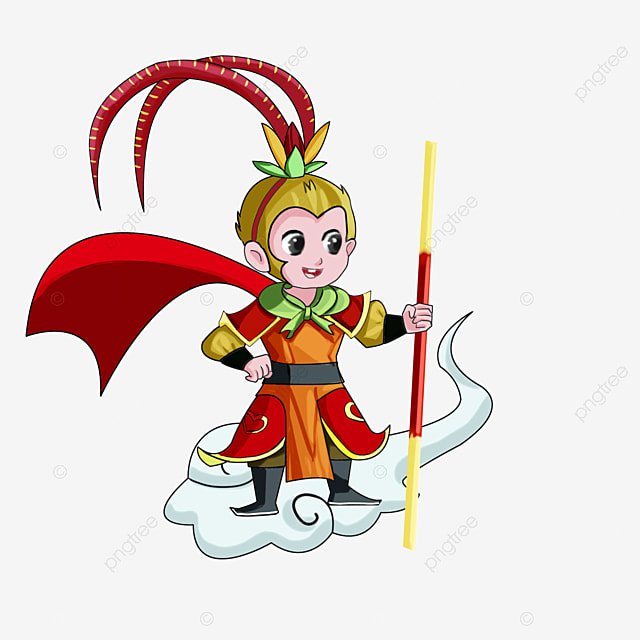
\includegraphics[width=\paperwidth,height=\paperheight]{../images/rei-macaco.jpg}
      }%
  }
  \BgThispage
  
  \begin{center}
    \huge
    Tabuada de Adição
  \end{center}

  \large
  \vspace{40pt}
  \noindent
  Registre o tempo gasto (em minutos):
  \begin{table}[!htpb]
    \begin{tabular}{|c|c|c|c|c|}
      \hline
      
    \begin{tabular}{ccccc}
1 & + & 5 & = & \\
    1 & + & 1 & = & \\
    1 & + & 7 & = & \\
    1 & + & 9 & = & \\
    1 & + & 10 & = & \\
    1 & + & 3 & = & \\
    1 & + & 4 & = & \\
    1 & + & 8 & = & \\
    1 & + & 2 & = & \\
    1 & + & 6 & = &
\end{tabular}&
    \begin{tabular}{ccccc}
2 & + & 10 & = & \\
    2 & + & 8 & = & \\
    2 & + & 5 & = & \\
    2 & + & 3 & = & \\
    2 & + & 7 & = & \\
    2 & + & 9 & = & \\
    2 & + & 6 & = & \\
    2 & + & 2 & = & \\
    2 & + & 4 & = & \\
    2 & + & 1 & = &
\end{tabular}&
    \begin{tabular}{ccccc}
3 & + & 4 & = & \\
    3 & + & 6 & = & \\
    3 & + & 7 & = & \\
    3 & + & 2 & = & \\
    3 & + & 9 & = & \\
    3 & + & 5 & = & \\
    3 & + & 1 & = & \\
    3 & + & 8 & = & \\
    3 & + & 10 & = & \\
    3 & + & 3 & = &
\end{tabular}&
    \begin{tabular}{ccccc}
4 & + & 8 & = & \\
    4 & + & 6 & = & \\
    4 & + & 5 & = & \\
    4 & + & 9 & = & \\
    4 & + & 2 & = & \\
    4 & + & 3 & = & \\
    4 & + & 10 & = & \\
    4 & + & 1 & = & \\
    4 & + & 7 & = & \\
    4 & + & 4 & = &
\end{tabular}&
    \begin{tabular}{ccccc}
5 & + & 8 & = & \\
    5 & + & 3 & = & \\
    5 & + & 10 & = & \\
    5 & + & 1 & = & \\
    5 & + & 7 & = & \\
    5 & + & 5 & = & \\
    5 & + & 9 & = & \\
    5 & + & 2 & = & \\
    5 & + & 6 & = & \\
    5 & + & 4 & = &
\end{tabular}
\\ \hline
    \begin{tabular}{ccccc}
6 & + & 9 & = & \\
    6 & + & 1 & = & \\
    6 & + & 8 & = & \\
    6 & + & 3 & = & \\
    6 & + & 10 & = & \\
    6 & + & 5 & = & \\
    6 & + & 2 & = & \\
    6 & + & 6 & = & \\
    6 & + & 7 & = & \\
    6 & + & 4 & = &
\end{tabular}&
    \begin{tabular}{ccccc}
7 & + & 1 & = & \\
    7 & + & 10 & = & \\
    7 & + & 7 & = & \\
    7 & + & 5 & = & \\
    7 & + & 8 & = & \\
    7 & + & 4 & = & \\
    7 & + & 6 & = & \\
    7 & + & 2 & = & \\
    7 & + & 3 & = & \\
    7 & + & 9 & = &
\end{tabular}&
    \begin{tabular}{ccccc}
8 & + & 7 & = & \\
    8 & + & 4 & = & \\
    8 & + & 10 & = & \\
    8 & + & 8 & = & \\
    8 & + & 2 & = & \\
    8 & + & 6 & = & \\
    8 & + & 1 & = & \\
    8 & + & 3 & = & \\
    8 & + & 9 & = & \\
    8 & + & 5 & = &
\end{tabular}&
    \begin{tabular}{ccccc}
9 & + & 4 & = & \\
    9 & + & 3 & = & \\
    9 & + & 7 & = & \\
    9 & + & 1 & = & \\
    9 & + & 2 & = & \\
    9 & + & 9 & = & \\
    9 & + & 8 & = & \\
    9 & + & 6 & = & \\
    9 & + & 10 & = & \\
    9 & + & 5 & = &
\end{tabular}&
    \begin{tabular}{ccccc}
10 & + & 5 & = & \\
    10 & + & 3 & = & \\
    10 & + & 1 & = & \\
    10 & + & 2 & = & \\
    10 & + & 10 & = & \\
    10 & + & 8 & = & \\
    10 & + & 4 & = & \\
    10 & + & 6 & = & \\
    10 & + & 9 & = & \\
    10 & + & 7 & = &
\end{tabular}
      \\ \hline
    \end{tabular}
  \end{table}
  \vfil
  \begin{flushright}
    \begin{minipage}[b]{6cm}
      A tabuada é o objeto de estudo mais importante na Matemática. É o caminho para se chegar ao universo dos números. (José Carlos dos Santos)
    \end{minipage}
  \end{flushright}

  \newpage
  

  \backgroundsetup{
    scale=1,
    color=black,
    opacity=0.2,
    angle=0,
    contents={%
        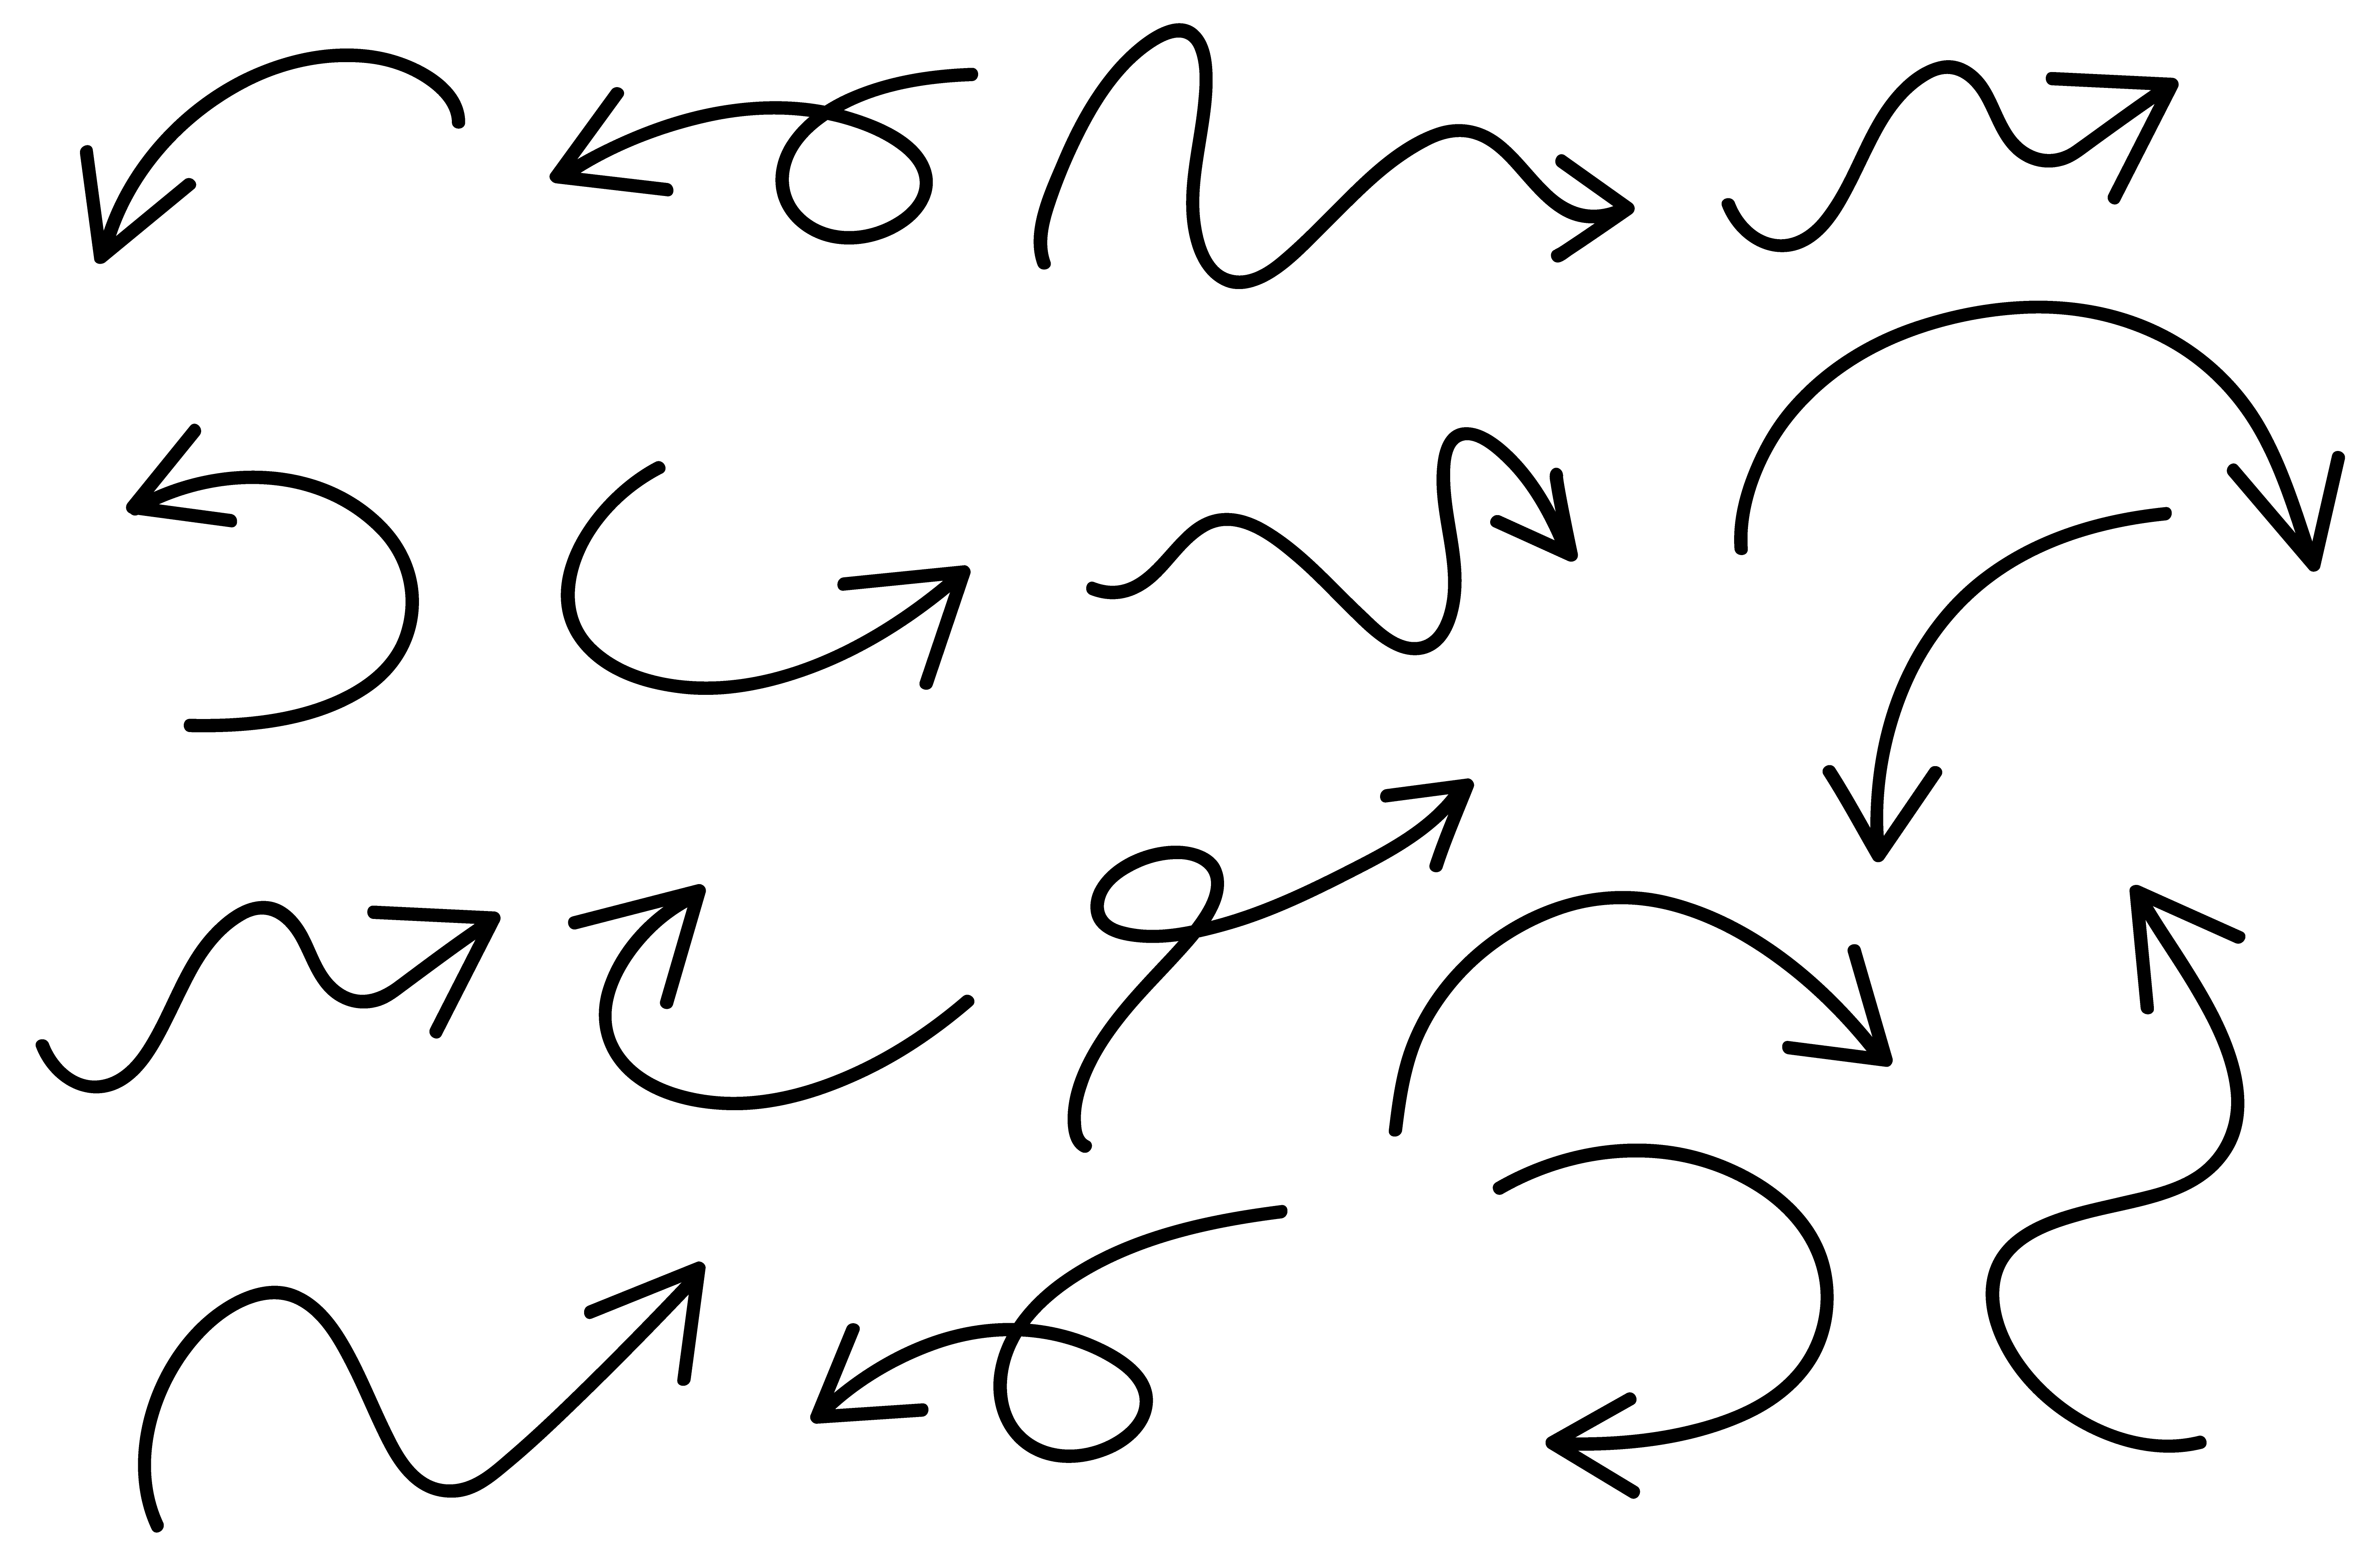
\includegraphics[width=\paperwidth,height=\paperheight]{../images/set-hand-drawn-arrow-doodles-white.jpg}
      }%
  }
  \BgThispage
  
  \begin{center}
    \huge
    Tabuada de Adição
  \end{center}

  \large
  \vspace{40pt}
  \noindent
  Registre o tempo gasto (em minutos):
  \begin{table}[!htpb]
    \begin{tabular}{|c|c|c|c|c|}
      \hline
      
    \begin{tabular}{ccccc}
1 & + & 5 & = & \\
    1 & + & 4 & = & \\
    1 & + & 7 & = & \\
    1 & + & 10 & = & \\
    1 & + & 3 & = & \\
    1 & + & 2 & = & \\
    1 & + & 9 & = & \\
    1 & + & 8 & = & \\
    1 & + & 1 & = & \\
    1 & + & 6 & = &
\end{tabular}&
    \begin{tabular}{ccccc}
2 & + & 5 & = & \\
    2 & + & 2 & = & \\
    2 & + & 9 & = & \\
    2 & + & 4 & = & \\
    2 & + & 6 & = & \\
    2 & + & 8 & = & \\
    2 & + & 10 & = & \\
    2 & + & 3 & = & \\
    2 & + & 7 & = & \\
    2 & + & 1 & = &
\end{tabular}&
    \begin{tabular}{ccccc}
3 & + & 10 & = & \\
    3 & + & 7 & = & \\
    3 & + & 8 & = & \\
    3 & + & 1 & = & \\
    3 & + & 2 & = & \\
    3 & + & 3 & = & \\
    3 & + & 6 & = & \\
    3 & + & 9 & = & \\
    3 & + & 4 & = & \\
    3 & + & 5 & = &
\end{tabular}&
    \begin{tabular}{ccccc}
4 & + & 10 & = & \\
    4 & + & 1 & = & \\
    4 & + & 6 & = & \\
    4 & + & 9 & = & \\
    4 & + & 2 & = & \\
    4 & + & 3 & = & \\
    4 & + & 7 & = & \\
    4 & + & 5 & = & \\
    4 & + & 4 & = & \\
    4 & + & 8 & = &
\end{tabular}&
    \begin{tabular}{ccccc}
5 & + & 9 & = & \\
    5 & + & 1 & = & \\
    5 & + & 10 & = & \\
    5 & + & 5 & = & \\
    5 & + & 6 & = & \\
    5 & + & 2 & = & \\
    5 & + & 3 & = & \\
    5 & + & 8 & = & \\
    5 & + & 4 & = & \\
    5 & + & 7 & = &
\end{tabular}
\\ \hline
    \begin{tabular}{ccccc}
6 & + & 8 & = & \\
    6 & + & 10 & = & \\
    6 & + & 4 & = & \\
    6 & + & 5 & = & \\
    6 & + & 3 & = & \\
    6 & + & 6 & = & \\
    6 & + & 9 & = & \\
    6 & + & 7 & = & \\
    6 & + & 1 & = & \\
    6 & + & 2 & = &
\end{tabular}&
    \begin{tabular}{ccccc}
7 & + & 10 & = & \\
    7 & + & 6 & = & \\
    7 & + & 2 & = & \\
    7 & + & 7 & = & \\
    7 & + & 5 & = & \\
    7 & + & 8 & = & \\
    7 & + & 9 & = & \\
    7 & + & 3 & = & \\
    7 & + & 4 & = & \\
    7 & + & 1 & = &
\end{tabular}&
    \begin{tabular}{ccccc}
8 & + & 2 & = & \\
    8 & + & 4 & = & \\
    8 & + & 8 & = & \\
    8 & + & 5 & = & \\
    8 & + & 10 & = & \\
    8 & + & 7 & = & \\
    8 & + & 9 & = & \\
    8 & + & 1 & = & \\
    8 & + & 3 & = & \\
    8 & + & 6 & = &
\end{tabular}&
    \begin{tabular}{ccccc}
9 & + & 10 & = & \\
    9 & + & 3 & = & \\
    9 & + & 7 & = & \\
    9 & + & 9 & = & \\
    9 & + & 2 & = & \\
    9 & + & 6 & = & \\
    9 & + & 1 & = & \\
    9 & + & 4 & = & \\
    9 & + & 5 & = & \\
    9 & + & 8 & = &
\end{tabular}&
    \begin{tabular}{ccccc}
10 & + & 1 & = & \\
    10 & + & 3 & = & \\
    10 & + & 10 & = & \\
    10 & + & 9 & = & \\
    10 & + & 7 & = & \\
    10 & + & 5 & = & \\
    10 & + & 8 & = & \\
    10 & + & 2 & = & \\
    10 & + & 4 & = & \\
    10 & + & 6 & = &
\end{tabular}
      \\ \hline
    \end{tabular}
  \end{table}
  \vfil
  \begin{flushright}
    \begin{minipage}[b]{6cm}
      A tabuada é o objeto de estudo mais importante na Matemática. É o caminho para se chegar ao universo dos números. (José Carlos dos Santos)
    \end{minipage}
  \end{flushright}

  \newpage
  

  \backgroundsetup{
    scale=1,
    color=black,
    opacity=0.2,
    angle=0,
    contents={%
        
\includegraphics[width=\paperwidth,height=\paperheight]{../images/son-goku.png}
      }%
  }
  \BgThispage
  
  \begin{center}
    \huge
    Tabuada de Adição
  \end{center}

  \large
  \vspace{40pt}
  \noindent
  Registre o tempo gasto (em minutos):
  \begin{table}[!htpb]
    \begin{tabular}{|c|c|c|c|c|}
      \hline
      
    \begin{tabular}{ccccc}
1 & + & 3 & = & \\
    1 & + & 10 & = & \\
    1 & + & 9 & = & \\
    1 & + & 6 & = & \\
    1 & + & 1 & = & \\
    1 & + & 4 & = & \\
    1 & + & 2 & = & \\
    1 & + & 7 & = & \\
    1 & + & 8 & = & \\
    1 & + & 5 & = &
\end{tabular}&
    \begin{tabular}{ccccc}
2 & + & 9 & = & \\
    2 & + & 6 & = & \\
    2 & + & 10 & = & \\
    2 & + & 5 & = & \\
    2 & + & 1 & = & \\
    2 & + & 3 & = & \\
    2 & + & 8 & = & \\
    2 & + & 7 & = & \\
    2 & + & 4 & = & \\
    2 & + & 2 & = &
\end{tabular}&
    \begin{tabular}{ccccc}
3 & + & 2 & = & \\
    3 & + & 9 & = & \\
    3 & + & 7 & = & \\
    3 & + & 4 & = & \\
    3 & + & 8 & = & \\
    3 & + & 5 & = & \\
    3 & + & 6 & = & \\
    3 & + & 3 & = & \\
    3 & + & 1 & = & \\
    3 & + & 10 & = &
\end{tabular}&
    \begin{tabular}{ccccc}
4 & + & 1 & = & \\
    4 & + & 8 & = & \\
    4 & + & 2 & = & \\
    4 & + & 5 & = & \\
    4 & + & 6 & = & \\
    4 & + & 4 & = & \\
    4 & + & 9 & = & \\
    4 & + & 10 & = & \\
    4 & + & 3 & = & \\
    4 & + & 7 & = &
\end{tabular}&
    \begin{tabular}{ccccc}
5 & + & 9 & = & \\
    5 & + & 10 & = & \\
    5 & + & 3 & = & \\
    5 & + & 1 & = & \\
    5 & + & 5 & = & \\
    5 & + & 2 & = & \\
    5 & + & 7 & = & \\
    5 & + & 4 & = & \\
    5 & + & 6 & = & \\
    5 & + & 8 & = &
\end{tabular}
\\ \hline
    \begin{tabular}{ccccc}
6 & + & 1 & = & \\
    6 & + & 9 & = & \\
    6 & + & 4 & = & \\
    6 & + & 6 & = & \\
    6 & + & 10 & = & \\
    6 & + & 7 & = & \\
    6 & + & 2 & = & \\
    6 & + & 3 & = & \\
    6 & + & 5 & = & \\
    6 & + & 8 & = &
\end{tabular}&
    \begin{tabular}{ccccc}
7 & + & 8 & = & \\
    7 & + & 7 & = & \\
    7 & + & 3 & = & \\
    7 & + & 9 & = & \\
    7 & + & 4 & = & \\
    7 & + & 1 & = & \\
    7 & + & 2 & = & \\
    7 & + & 10 & = & \\
    7 & + & 6 & = & \\
    7 & + & 5 & = &
\end{tabular}&
    \begin{tabular}{ccccc}
8 & + & 1 & = & \\
    8 & + & 3 & = & \\
    8 & + & 5 & = & \\
    8 & + & 4 & = & \\
    8 & + & 10 & = & \\
    8 & + & 7 & = & \\
    8 & + & 2 & = & \\
    8 & + & 8 & = & \\
    8 & + & 6 & = & \\
    8 & + & 9 & = &
\end{tabular}&
    \begin{tabular}{ccccc}
9 & + & 9 & = & \\
    9 & + & 3 & = & \\
    9 & + & 4 & = & \\
    9 & + & 6 & = & \\
    9 & + & 2 & = & \\
    9 & + & 8 & = & \\
    9 & + & 5 & = & \\
    9 & + & 10 & = & \\
    9 & + & 7 & = & \\
    9 & + & 1 & = &
\end{tabular}&
    \begin{tabular}{ccccc}
10 & + & 8 & = & \\
    10 & + & 1 & = & \\
    10 & + & 4 & = & \\
    10 & + & 10 & = & \\
    10 & + & 6 & = & \\
    10 & + & 9 & = & \\
    10 & + & 5 & = & \\
    10 & + & 3 & = & \\
    10 & + & 2 & = & \\
    10 & + & 7 & = &
\end{tabular}
      \\ \hline
    \end{tabular}
  \end{table}
  \vfil
  \begin{flushright}
    \begin{minipage}[b]{6cm}
      A tabuada é o objeto de estudo mais importante na Matemática. É o caminho para se chegar ao universo dos números. (José Carlos dos Santos)
    \end{minipage}
  \end{flushright}

  \newpage
  

  \backgroundsetup{
    scale=1,
    color=black,
    opacity=0.2,
    angle=0,
    contents={%
        \includegraphics[width=\paperwidth,height=\paperheight]{../images/students-raising-their-hands-with-teacher-white-background.jpg}
      }%
  }
  \BgThispage
  
  \begin{center}
    \huge
    Tabuada de Adição
  \end{center}

  \large
  \vspace{40pt}
  \noindent
  Registre o tempo gasto (em minutos):
  \begin{table}[!htpb]
    \begin{tabular}{|c|c|c|c|c|}
      \hline
      
    \begin{tabular}{ccccc}
1 & + & 9 & = & \\
    1 & + & 3 & = & \\
    1 & + & 5 & = & \\
    1 & + & 7 & = & \\
    1 & + & 1 & = & \\
    1 & + & 10 & = & \\
    1 & + & 6 & = & \\
    1 & + & 8 & = & \\
    1 & + & 4 & = & \\
    1 & + & 2 & = &
\end{tabular}&
    \begin{tabular}{ccccc}
2 & + & 7 & = & \\
    2 & + & 3 & = & \\
    2 & + & 9 & = & \\
    2 & + & 8 & = & \\
    2 & + & 2 & = & \\
    2 & + & 1 & = & \\
    2 & + & 10 & = & \\
    2 & + & 4 & = & \\
    2 & + & 5 & = & \\
    2 & + & 6 & = &
\end{tabular}&
    \begin{tabular}{ccccc}
3 & + & 4 & = & \\
    3 & + & 10 & = & \\
    3 & + & 9 & = & \\
    3 & + & 5 & = & \\
    3 & + & 3 & = & \\
    3 & + & 8 & = & \\
    3 & + & 1 & = & \\
    3 & + & 2 & = & \\
    3 & + & 7 & = & \\
    3 & + & 6 & = &
\end{tabular}&
    \begin{tabular}{ccccc}
4 & + & 9 & = & \\
    4 & + & 10 & = & \\
    4 & + & 4 & = & \\
    4 & + & 8 & = & \\
    4 & + & 7 & = & \\
    4 & + & 6 & = & \\
    4 & + & 2 & = & \\
    4 & + & 5 & = & \\
    4 & + & 3 & = & \\
    4 & + & 1 & = &
\end{tabular}&
    \begin{tabular}{ccccc}
5 & + & 1 & = & \\
    5 & + & 10 & = & \\
    5 & + & 9 & = & \\
    5 & + & 5 & = & \\
    5 & + & 2 & = & \\
    5 & + & 7 & = & \\
    5 & + & 6 & = & \\
    5 & + & 4 & = & \\
    5 & + & 3 & = & \\
    5 & + & 8 & = &
\end{tabular}
\\ \hline
    \begin{tabular}{ccccc}
6 & + & 6 & = & \\
    6 & + & 8 & = & \\
    6 & + & 7 & = & \\
    6 & + & 4 & = & \\
    6 & + & 9 & = & \\
    6 & + & 1 & = & \\
    6 & + & 10 & = & \\
    6 & + & 2 & = & \\
    6 & + & 3 & = & \\
    6 & + & 5 & = &
\end{tabular}&
    \begin{tabular}{ccccc}
7 & + & 7 & = & \\
    7 & + & 5 & = & \\
    7 & + & 9 & = & \\
    7 & + & 10 & = & \\
    7 & + & 2 & = & \\
    7 & + & 3 & = & \\
    7 & + & 4 & = & \\
    7 & + & 6 & = & \\
    7 & + & 1 & = & \\
    7 & + & 8 & = &
\end{tabular}&
    \begin{tabular}{ccccc}
8 & + & 3 & = & \\
    8 & + & 8 & = & \\
    8 & + & 10 & = & \\
    8 & + & 6 & = & \\
    8 & + & 1 & = & \\
    8 & + & 4 & = & \\
    8 & + & 9 & = & \\
    8 & + & 7 & = & \\
    8 & + & 5 & = & \\
    8 & + & 2 & = &
\end{tabular}&
    \begin{tabular}{ccccc}
9 & + & 7 & = & \\
    9 & + & 4 & = & \\
    9 & + & 1 & = & \\
    9 & + & 9 & = & \\
    9 & + & 10 & = & \\
    9 & + & 5 & = & \\
    9 & + & 8 & = & \\
    9 & + & 3 & = & \\
    9 & + & 6 & = & \\
    9 & + & 2 & = &
\end{tabular}&
    \begin{tabular}{ccccc}
10 & + & 9 & = & \\
    10 & + & 4 & = & \\
    10 & + & 2 & = & \\
    10 & + & 6 & = & \\
    10 & + & 1 & = & \\
    10 & + & 7 & = & \\
    10 & + & 10 & = & \\
    10 & + & 8 & = & \\
    10 & + & 3 & = & \\
    10 & + & 5 & = &
\end{tabular}
      \\ \hline
    \end{tabular}
  \end{table}
  \vfil
  \begin{flushright}
    \begin{minipage}[b]{6cm}
      A tabuada é o objeto de estudo mais importante na Matemática. É o caminho para se chegar ao universo dos números. (José Carlos dos Santos)
    \end{minipage}
  \end{flushright}

  \newpage
  

  \backgroundsetup{
    scale=1,
    color=black,
    opacity=0.2,
    angle=0,
    contents={%
        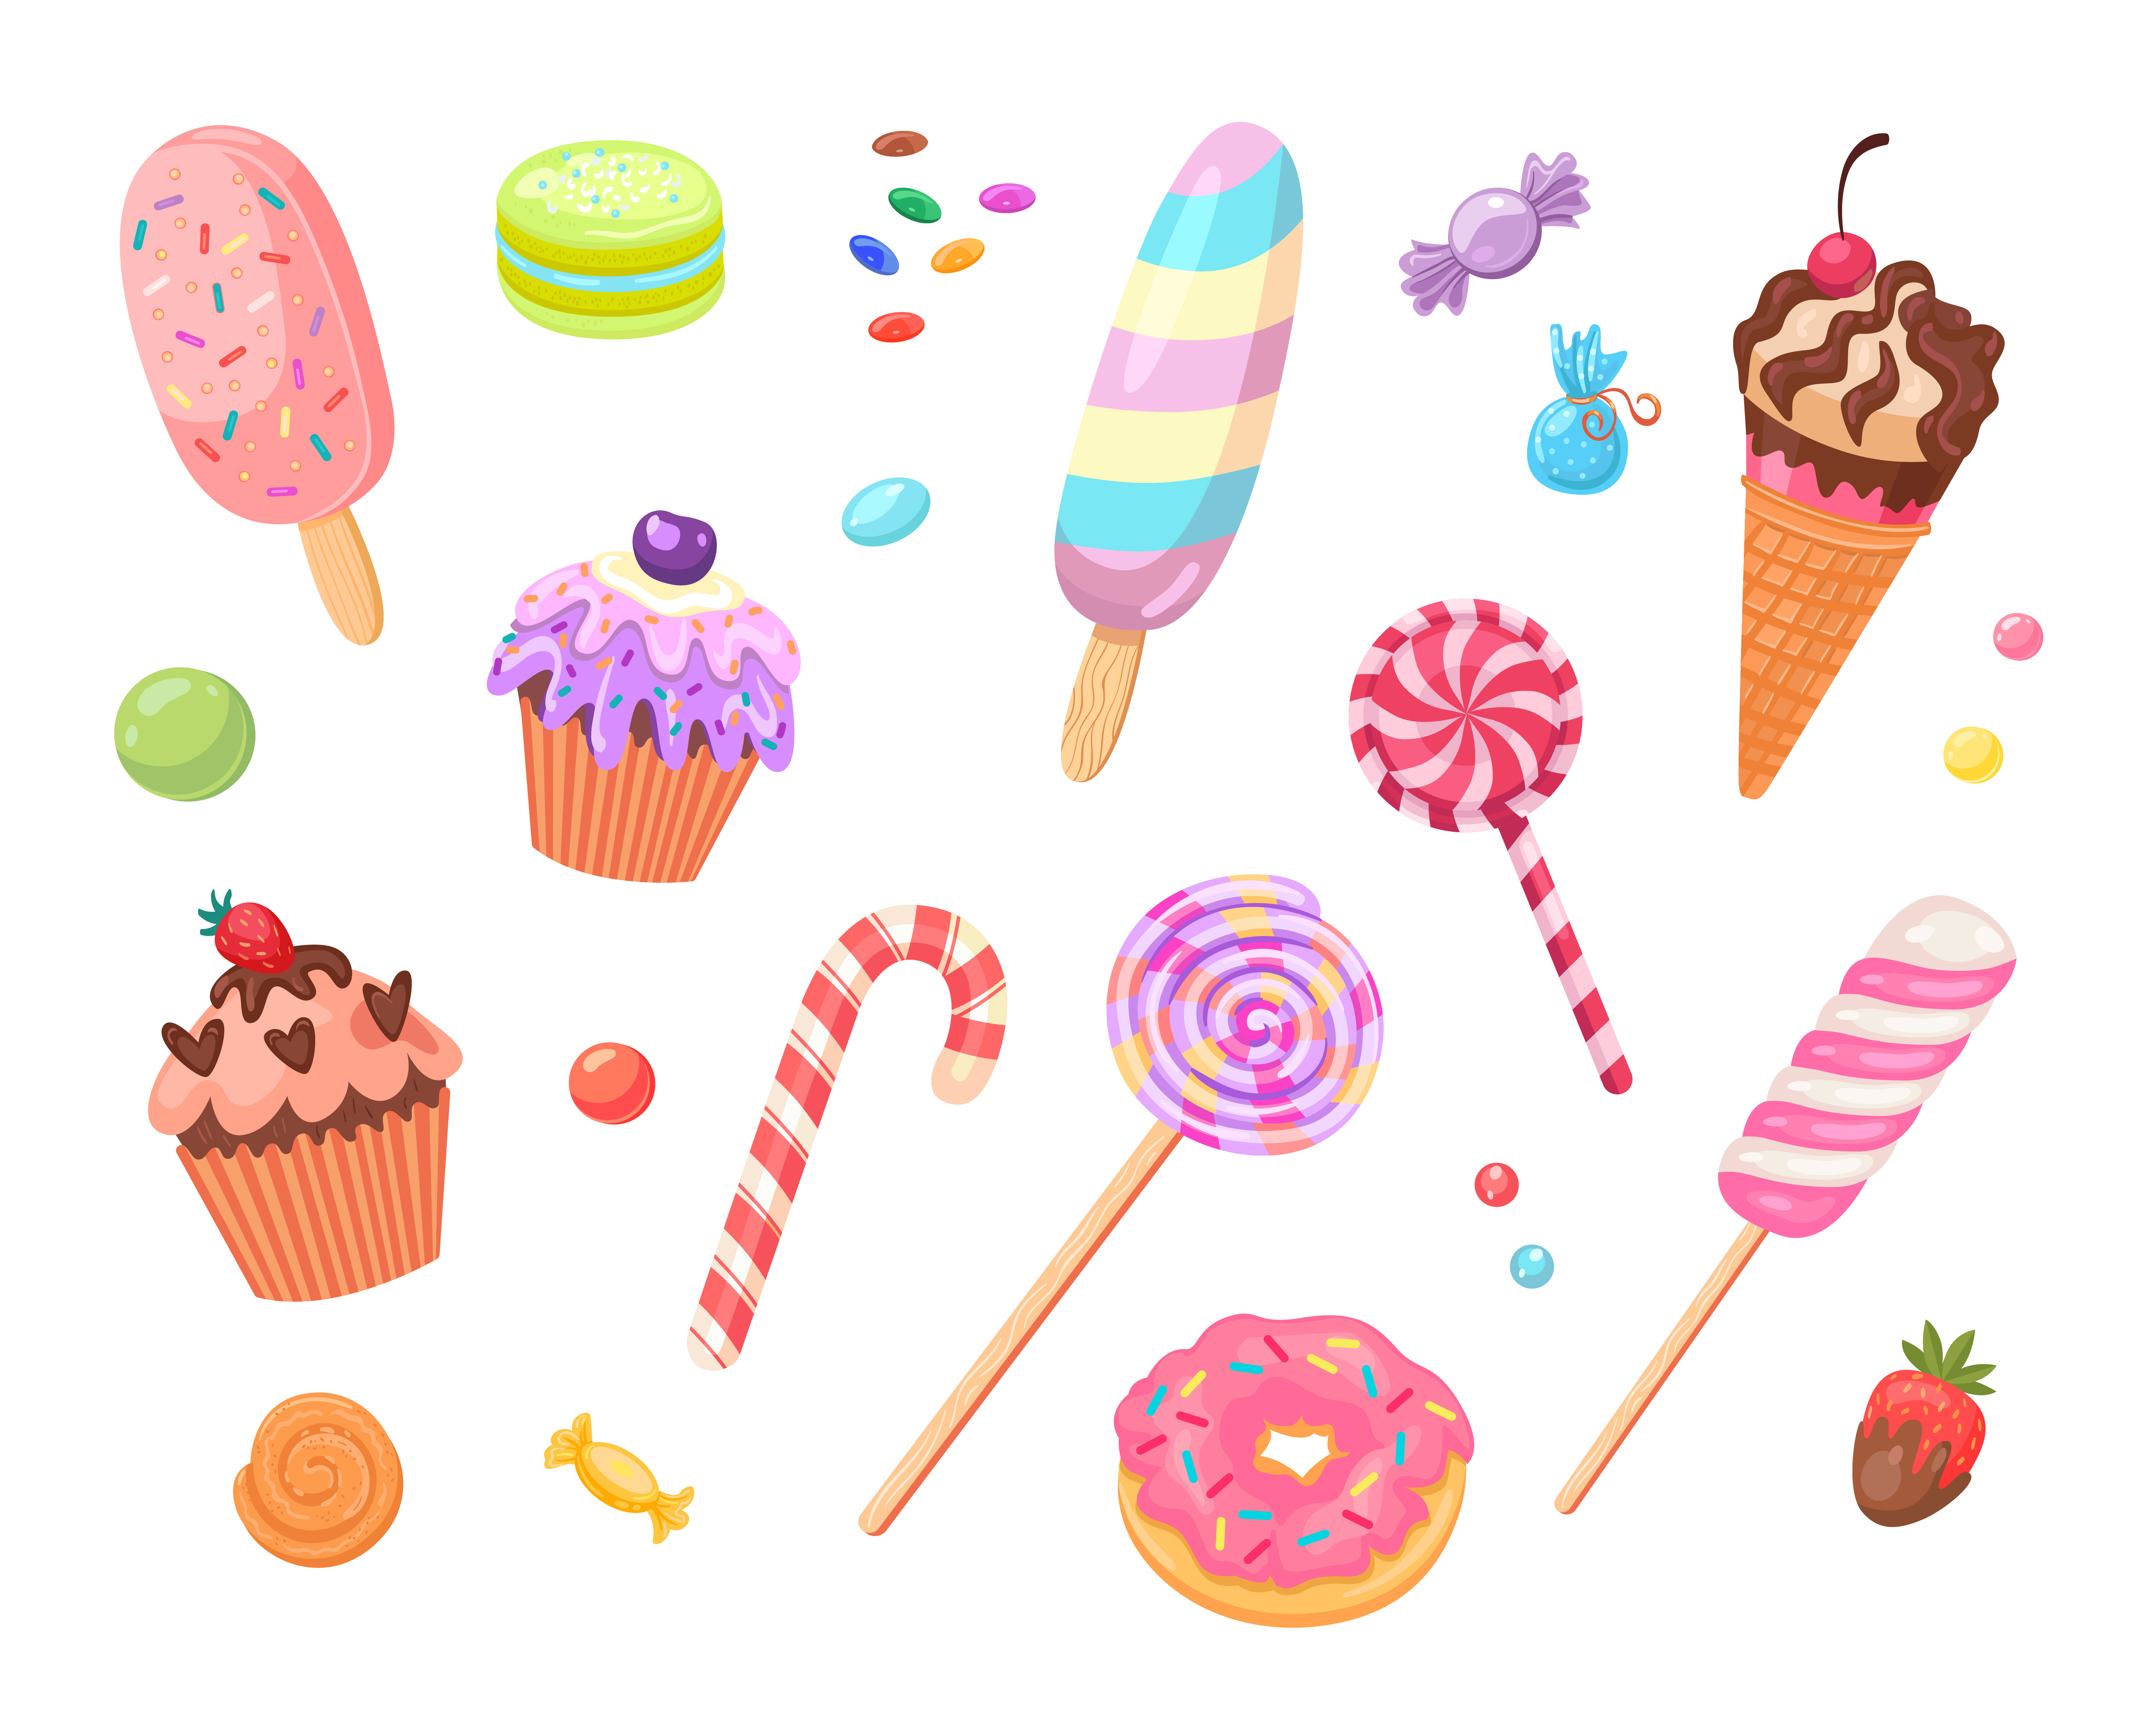
\includegraphics[width=\paperwidth,height=\paperheight]{../images/sweets-cakes-flat-icon-set.jpg}
      }%
  }
  \BgThispage
  
  \begin{center}
    \huge
    Tabuada de Adição
  \end{center}

  \large
  \vspace{40pt}
  \noindent
  Registre o tempo gasto (em minutos):
  \begin{table}[!htpb]
    \begin{tabular}{|c|c|c|c|c|}
      \hline
      
    \begin{tabular}{ccccc}
1 & + & 7 & = & \\
    1 & + & 4 & = & \\
    1 & + & 8 & = & \\
    1 & + & 10 & = & \\
    1 & + & 2 & = & \\
    1 & + & 6 & = & \\
    1 & + & 3 & = & \\
    1 & + & 5 & = & \\
    1 & + & 1 & = & \\
    1 & + & 9 & = &
\end{tabular}&
    \begin{tabular}{ccccc}
2 & + & 6 & = & \\
    2 & + & 3 & = & \\
    2 & + & 9 & = & \\
    2 & + & 10 & = & \\
    2 & + & 5 & = & \\
    2 & + & 4 & = & \\
    2 & + & 2 & = & \\
    2 & + & 8 & = & \\
    2 & + & 7 & = & \\
    2 & + & 1 & = &
\end{tabular}&
    \begin{tabular}{ccccc}
3 & + & 8 & = & \\
    3 & + & 1 & = & \\
    3 & + & 6 & = & \\
    3 & + & 5 & = & \\
    3 & + & 4 & = & \\
    3 & + & 9 & = & \\
    3 & + & 10 & = & \\
    3 & + & 7 & = & \\
    3 & + & 2 & = & \\
    3 & + & 3 & = &
\end{tabular}&
    \begin{tabular}{ccccc}
4 & + & 5 & = & \\
    4 & + & 2 & = & \\
    4 & + & 7 & = & \\
    4 & + & 10 & = & \\
    4 & + & 3 & = & \\
    4 & + & 4 & = & \\
    4 & + & 6 & = & \\
    4 & + & 1 & = & \\
    4 & + & 9 & = & \\
    4 & + & 8 & = &
\end{tabular}&
    \begin{tabular}{ccccc}
5 & + & 2 & = & \\
    5 & + & 9 & = & \\
    5 & + & 10 & = & \\
    5 & + & 8 & = & \\
    5 & + & 6 & = & \\
    5 & + & 4 & = & \\
    5 & + & 3 & = & \\
    5 & + & 7 & = & \\
    5 & + & 1 & = & \\
    5 & + & 5 & = &
\end{tabular}
\\ \hline
    \begin{tabular}{ccccc}
6 & + & 1 & = & \\
    6 & + & 6 & = & \\
    6 & + & 5 & = & \\
    6 & + & 4 & = & \\
    6 & + & 3 & = & \\
    6 & + & 7 & = & \\
    6 & + & 10 & = & \\
    6 & + & 2 & = & \\
    6 & + & 9 & = & \\
    6 & + & 8 & = &
\end{tabular}&
    \begin{tabular}{ccccc}
7 & + & 10 & = & \\
    7 & + & 5 & = & \\
    7 & + & 1 & = & \\
    7 & + & 4 & = & \\
    7 & + & 8 & = & \\
    7 & + & 3 & = & \\
    7 & + & 7 & = & \\
    7 & + & 9 & = & \\
    7 & + & 2 & = & \\
    7 & + & 6 & = &
\end{tabular}&
    \begin{tabular}{ccccc}
8 & + & 2 & = & \\
    8 & + & 1 & = & \\
    8 & + & 3 & = & \\
    8 & + & 4 & = & \\
    8 & + & 6 & = & \\
    8 & + & 8 & = & \\
    8 & + & 7 & = & \\
    8 & + & 9 & = & \\
    8 & + & 10 & = & \\
    8 & + & 5 & = &
\end{tabular}&
    \begin{tabular}{ccccc}
9 & + & 3 & = & \\
    9 & + & 6 & = & \\
    9 & + & 2 & = & \\
    9 & + & 7 & = & \\
    9 & + & 1 & = & \\
    9 & + & 8 & = & \\
    9 & + & 4 & = & \\
    9 & + & 9 & = & \\
    9 & + & 10 & = & \\
    9 & + & 5 & = &
\end{tabular}&
    \begin{tabular}{ccccc}
10 & + & 7 & = & \\
    10 & + & 1 & = & \\
    10 & + & 5 & = & \\
    10 & + & 4 & = & \\
    10 & + & 3 & = & \\
    10 & + & 9 & = & \\
    10 & + & 2 & = & \\
    10 & + & 10 & = & \\
    10 & + & 6 & = & \\
    10 & + & 8 & = &
\end{tabular}
      \\ \hline
    \end{tabular}
  \end{table}
  \vfil
  \begin{flushright}
    \begin{minipage}[b]{6cm}
      A tabuada é o objeto de estudo mais importante na Matemática. É o caminho para se chegar ao universo dos números. (José Carlos dos Santos)
    \end{minipage}
  \end{flushright}

  \newpage
  

  \backgroundsetup{
    scale=1,
    color=black,
    opacity=0.2,
    angle=0,
    contents={%
        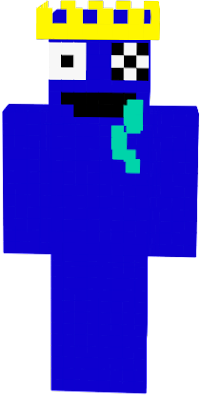
\includegraphics[width=\paperwidth,height=\paperheight]{../images/babao.png}
      }%
  }
  \BgThispage
  
  \begin{center}
    \huge
    Tabuada de Adição
  \end{center}

  \large
  \vspace{40pt}
  \noindent
  Registre o tempo gasto (em minutos):
  \begin{table}[!htpb]
    \begin{tabular}{|c|c|c|c|c|}
      \hline
      
    \begin{tabular}{ccccc}
1 & + & 9 & = & \\
    1 & + & 3 & = & \\
    1 & + & 1 & = & \\
    1 & + & 10 & = & \\
    1 & + & 6 & = & \\
    1 & + & 5 & = & \\
    1 & + & 2 & = & \\
    1 & + & 4 & = & \\
    1 & + & 8 & = & \\
    1 & + & 7 & = &
\end{tabular}&
    \begin{tabular}{ccccc}
2 & + & 9 & = & \\
    2 & + & 10 & = & \\
    2 & + & 4 & = & \\
    2 & + & 8 & = & \\
    2 & + & 1 & = & \\
    2 & + & 2 & = & \\
    2 & + & 3 & = & \\
    2 & + & 7 & = & \\
    2 & + & 5 & = & \\
    2 & + & 6 & = &
\end{tabular}&
    \begin{tabular}{ccccc}
3 & + & 4 & = & \\
    3 & + & 1 & = & \\
    3 & + & 10 & = & \\
    3 & + & 7 & = & \\
    3 & + & 6 & = & \\
    3 & + & 2 & = & \\
    3 & + & 5 & = & \\
    3 & + & 3 & = & \\
    3 & + & 8 & = & \\
    3 & + & 9 & = &
\end{tabular}&
    \begin{tabular}{ccccc}
4 & + & 1 & = & \\
    4 & + & 6 & = & \\
    4 & + & 7 & = & \\
    4 & + & 8 & = & \\
    4 & + & 3 & = & \\
    4 & + & 10 & = & \\
    4 & + & 4 & = & \\
    4 & + & 2 & = & \\
    4 & + & 9 & = & \\
    4 & + & 5 & = &
\end{tabular}&
    \begin{tabular}{ccccc}
5 & + & 4 & = & \\
    5 & + & 5 & = & \\
    5 & + & 3 & = & \\
    5 & + & 7 & = & \\
    5 & + & 8 & = & \\
    5 & + & 1 & = & \\
    5 & + & 2 & = & \\
    5 & + & 9 & = & \\
    5 & + & 10 & = & \\
    5 & + & 6 & = &
\end{tabular}
\\ \hline
    \begin{tabular}{ccccc}
6 & + & 5 & = & \\
    6 & + & 8 & = & \\
    6 & + & 1 & = & \\
    6 & + & 4 & = & \\
    6 & + & 7 & = & \\
    6 & + & 3 & = & \\
    6 & + & 6 & = & \\
    6 & + & 2 & = & \\
    6 & + & 9 & = & \\
    6 & + & 10 & = &
\end{tabular}&
    \begin{tabular}{ccccc}
7 & + & 5 & = & \\
    7 & + & 8 & = & \\
    7 & + & 4 & = & \\
    7 & + & 2 & = & \\
    7 & + & 6 & = & \\
    7 & + & 1 & = & \\
    7 & + & 9 & = & \\
    7 & + & 3 & = & \\
    7 & + & 7 & = & \\
    7 & + & 10 & = &
\end{tabular}&
    \begin{tabular}{ccccc}
8 & + & 7 & = & \\
    8 & + & 4 & = & \\
    8 & + & 6 & = & \\
    8 & + & 3 & = & \\
    8 & + & 8 & = & \\
    8 & + & 10 & = & \\
    8 & + & 5 & = & \\
    8 & + & 2 & = & \\
    8 & + & 1 & = & \\
    8 & + & 9 & = &
\end{tabular}&
    \begin{tabular}{ccccc}
9 & + & 4 & = & \\
    9 & + & 1 & = & \\
    9 & + & 9 & = & \\
    9 & + & 5 & = & \\
    9 & + & 7 & = & \\
    9 & + & 3 & = & \\
    9 & + & 6 & = & \\
    9 & + & 2 & = & \\
    9 & + & 10 & = & \\
    9 & + & 8 & = &
\end{tabular}&
    \begin{tabular}{ccccc}
10 & + & 8 & = & \\
    10 & + & 3 & = & \\
    10 & + & 10 & = & \\
    10 & + & 9 & = & \\
    10 & + & 1 & = & \\
    10 & + & 6 & = & \\
    10 & + & 4 & = & \\
    10 & + & 2 & = & \\
    10 & + & 5 & = & \\
    10 & + & 7 & = &
\end{tabular}
      \\ \hline
    \end{tabular}
  \end{table}
  \vfil
  \begin{flushright}
    \begin{minipage}[b]{6cm}
      A tabuada é o objeto de estudo mais importante na Matemática. É o caminho para se chegar ao universo dos números. (José Carlos dos Santos)
    \end{minipage}
  \end{flushright}

  \newpage
  

  \backgroundsetup{
    scale=1,
    color=black,
    opacity=0.2,
    angle=0,
    contents={%
        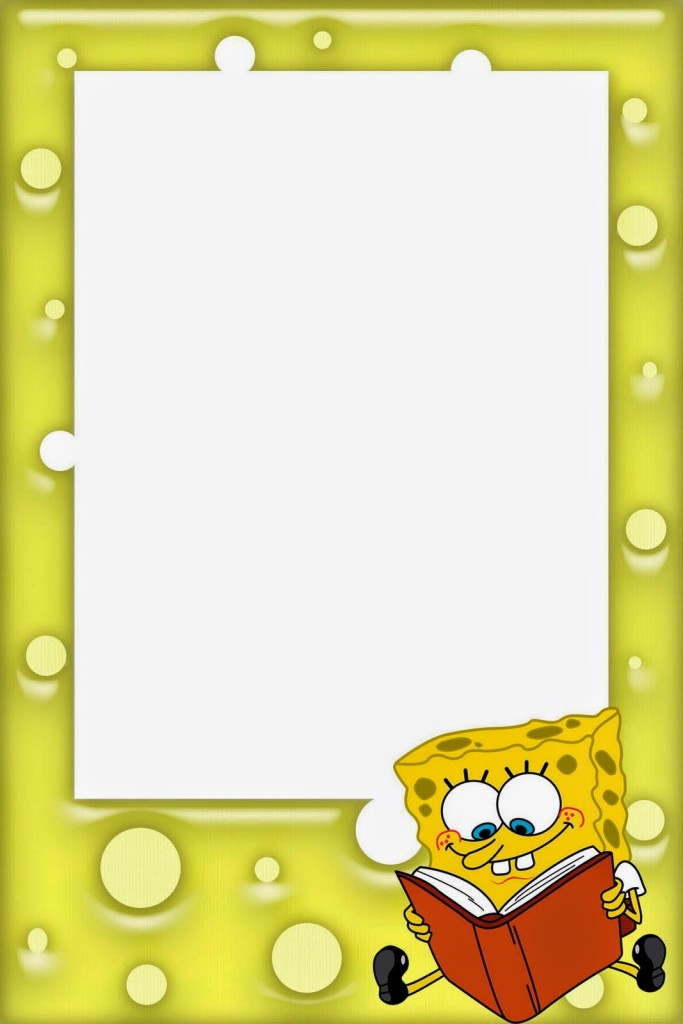
\includegraphics[width=\paperwidth,height=\paperheight]{../images/Bob-Esponja-estudando.jpg}
      }%
  }
  \BgThispage
  
  \begin{center}
    \huge
    Tabuada de Adição
  \end{center}

  \large
  \vspace{40pt}
  \noindent
  Registre o tempo gasto (em minutos):
  \begin{table}[!htpb]
    \begin{tabular}{|c|c|c|c|c|}
      \hline
      
    \begin{tabular}{ccccc}
1 & + & 2 & = & \\
    1 & + & 5 & = & \\
    1 & + & 6 & = & \\
    1 & + & 8 & = & \\
    1 & + & 9 & = & \\
    1 & + & 10 & = & \\
    1 & + & 4 & = & \\
    1 & + & 3 & = & \\
    1 & + & 7 & = & \\
    1 & + & 1 & = &
\end{tabular}&
    \begin{tabular}{ccccc}
2 & + & 10 & = & \\
    2 & + & 2 & = & \\
    2 & + & 7 & = & \\
    2 & + & 5 & = & \\
    2 & + & 4 & = & \\
    2 & + & 1 & = & \\
    2 & + & 6 & = & \\
    2 & + & 9 & = & \\
    2 & + & 3 & = & \\
    2 & + & 8 & = &
\end{tabular}&
    \begin{tabular}{ccccc}
3 & + & 1 & = & \\
    3 & + & 7 & = & \\
    3 & + & 9 & = & \\
    3 & + & 2 & = & \\
    3 & + & 10 & = & \\
    3 & + & 6 & = & \\
    3 & + & 4 & = & \\
    3 & + & 3 & = & \\
    3 & + & 5 & = & \\
    3 & + & 8 & = &
\end{tabular}&
    \begin{tabular}{ccccc}
4 & + & 9 & = & \\
    4 & + & 1 & = & \\
    4 & + & 10 & = & \\
    4 & + & 7 & = & \\
    4 & + & 4 & = & \\
    4 & + & 5 & = & \\
    4 & + & 6 & = & \\
    4 & + & 8 & = & \\
    4 & + & 3 & = & \\
    4 & + & 2 & = &
\end{tabular}&
    \begin{tabular}{ccccc}
5 & + & 9 & = & \\
    5 & + & 6 & = & \\
    5 & + & 2 & = & \\
    5 & + & 5 & = & \\
    5 & + & 10 & = & \\
    5 & + & 1 & = & \\
    5 & + & 3 & = & \\
    5 & + & 4 & = & \\
    5 & + & 7 & = & \\
    5 & + & 8 & = &
\end{tabular}
\\ \hline
    \begin{tabular}{ccccc}
6 & + & 7 & = & \\
    6 & + & 5 & = & \\
    6 & + & 2 & = & \\
    6 & + & 8 & = & \\
    6 & + & 3 & = & \\
    6 & + & 10 & = & \\
    6 & + & 1 & = & \\
    6 & + & 4 & = & \\
    6 & + & 9 & = & \\
    6 & + & 6 & = &
\end{tabular}&
    \begin{tabular}{ccccc}
7 & + & 1 & = & \\
    7 & + & 3 & = & \\
    7 & + & 2 & = & \\
    7 & + & 4 & = & \\
    7 & + & 6 & = & \\
    7 & + & 7 & = & \\
    7 & + & 8 & = & \\
    7 & + & 10 & = & \\
    7 & + & 5 & = & \\
    7 & + & 9 & = &
\end{tabular}&
    \begin{tabular}{ccccc}
8 & + & 10 & = & \\
    8 & + & 4 & = & \\
    8 & + & 1 & = & \\
    8 & + & 7 & = & \\
    8 & + & 8 & = & \\
    8 & + & 3 & = & \\
    8 & + & 9 & = & \\
    8 & + & 5 & = & \\
    8 & + & 2 & = & \\
    8 & + & 6 & = &
\end{tabular}&
    \begin{tabular}{ccccc}
9 & + & 7 & = & \\
    9 & + & 3 & = & \\
    9 & + & 4 & = & \\
    9 & + & 1 & = & \\
    9 & + & 10 & = & \\
    9 & + & 6 & = & \\
    9 & + & 2 & = & \\
    9 & + & 8 & = & \\
    9 & + & 5 & = & \\
    9 & + & 9 & = &
\end{tabular}&
    \begin{tabular}{ccccc}
10 & + & 5 & = & \\
    10 & + & 4 & = & \\
    10 & + & 9 & = & \\
    10 & + & 6 & = & \\
    10 & + & 8 & = & \\
    10 & + & 10 & = & \\
    10 & + & 7 & = & \\
    10 & + & 1 & = & \\
    10 & + & 2 & = & \\
    10 & + & 3 & = &
\end{tabular}
      \\ \hline
    \end{tabular}
  \end{table}
  \vfil
  \begin{flushright}
    \begin{minipage}[b]{6cm}
      A tabuada é o objeto de estudo mais importante na Matemática. É o caminho para se chegar ao universo dos números. (José Carlos dos Santos)
    \end{minipage}
  \end{flushright}

  \newpage
  

  \backgroundsetup{
    scale=1,
    color=black,
    opacity=0.2,
    angle=0,
    contents={%
        \includegraphics[width=\paperwidth,height=\paperheight]{../images/cute-galaxy-blue-frame-white-background-kids.jpg}
      }%
  }
  \BgThispage
  
  \begin{center}
    \huge
    Tabuada de Adição
  \end{center}

  \large
  \vspace{40pt}
  \noindent
  Registre o tempo gasto (em minutos):
  \begin{table}[!htpb]
    \begin{tabular}{|c|c|c|c|c|}
      \hline
      
    \begin{tabular}{ccccc}
1 & + & 6 & = & \\
    1 & + & 8 & = & \\
    1 & + & 5 & = & \\
    1 & + & 7 & = & \\
    1 & + & 9 & = & \\
    1 & + & 4 & = & \\
    1 & + & 1 & = & \\
    1 & + & 10 & = & \\
    1 & + & 2 & = & \\
    1 & + & 3 & = &
\end{tabular}&
    \begin{tabular}{ccccc}
2 & + & 1 & = & \\
    2 & + & 7 & = & \\
    2 & + & 3 & = & \\
    2 & + & 5 & = & \\
    2 & + & 4 & = & \\
    2 & + & 8 & = & \\
    2 & + & 2 & = & \\
    2 & + & 9 & = & \\
    2 & + & 6 & = & \\
    2 & + & 10 & = &
\end{tabular}&
    \begin{tabular}{ccccc}
3 & + & 9 & = & \\
    3 & + & 10 & = & \\
    3 & + & 4 & = & \\
    3 & + & 8 & = & \\
    3 & + & 7 & = & \\
    3 & + & 2 & = & \\
    3 & + & 1 & = & \\
    3 & + & 5 & = & \\
    3 & + & 6 & = & \\
    3 & + & 3 & = &
\end{tabular}&
    \begin{tabular}{ccccc}
4 & + & 8 & = & \\
    4 & + & 9 & = & \\
    4 & + & 2 & = & \\
    4 & + & 3 & = & \\
    4 & + & 5 & = & \\
    4 & + & 1 & = & \\
    4 & + & 7 & = & \\
    4 & + & 4 & = & \\
    4 & + & 6 & = & \\
    4 & + & 10 & = &
\end{tabular}&
    \begin{tabular}{ccccc}
5 & + & 5 & = & \\
    5 & + & 4 & = & \\
    5 & + & 8 & = & \\
    5 & + & 9 & = & \\
    5 & + & 6 & = & \\
    5 & + & 7 & = & \\
    5 & + & 10 & = & \\
    5 & + & 1 & = & \\
    5 & + & 2 & = & \\
    5 & + & 3 & = &
\end{tabular}
\\ \hline
    \begin{tabular}{ccccc}
6 & + & 5 & = & \\
    6 & + & 6 & = & \\
    6 & + & 1 & = & \\
    6 & + & 4 & = & \\
    6 & + & 8 & = & \\
    6 & + & 9 & = & \\
    6 & + & 7 & = & \\
    6 & + & 3 & = & \\
    6 & + & 2 & = & \\
    6 & + & 10 & = &
\end{tabular}&
    \begin{tabular}{ccccc}
7 & + & 5 & = & \\
    7 & + & 9 & = & \\
    7 & + & 6 & = & \\
    7 & + & 2 & = & \\
    7 & + & 7 & = & \\
    7 & + & 4 & = & \\
    7 & + & 3 & = & \\
    7 & + & 8 & = & \\
    7 & + & 10 & = & \\
    7 & + & 1 & = &
\end{tabular}&
    \begin{tabular}{ccccc}
8 & + & 6 & = & \\
    8 & + & 8 & = & \\
    8 & + & 3 & = & \\
    8 & + & 7 & = & \\
    8 & + & 10 & = & \\
    8 & + & 4 & = & \\
    8 & + & 5 & = & \\
    8 & + & 9 & = & \\
    8 & + & 2 & = & \\
    8 & + & 1 & = &
\end{tabular}&
    \begin{tabular}{ccccc}
9 & + & 8 & = & \\
    9 & + & 6 & = & \\
    9 & + & 3 & = & \\
    9 & + & 10 & = & \\
    9 & + & 4 & = & \\
    9 & + & 7 & = & \\
    9 & + & 9 & = & \\
    9 & + & 1 & = & \\
    9 & + & 5 & = & \\
    9 & + & 2 & = &
\end{tabular}&
    \begin{tabular}{ccccc}
10 & + & 6 & = & \\
    10 & + & 3 & = & \\
    10 & + & 2 & = & \\
    10 & + & 10 & = & \\
    10 & + & 4 & = & \\
    10 & + & 7 & = & \\
    10 & + & 8 & = & \\
    10 & + & 9 & = & \\
    10 & + & 1 & = & \\
    10 & + & 5 & = &
\end{tabular}
      \\ \hline
    \end{tabular}
  \end{table}
  \vfil
  \begin{flushright}
    \begin{minipage}[b]{6cm}
      A tabuada é o objeto de estudo mais importante na Matemática. É o caminho para se chegar ao universo dos números. (José Carlos dos Santos)
    \end{minipage}
  \end{flushright}

  \newpage
  

  \backgroundsetup{
    scale=1,
    color=black,
    opacity=0.2,
    angle=0,
    contents={%
        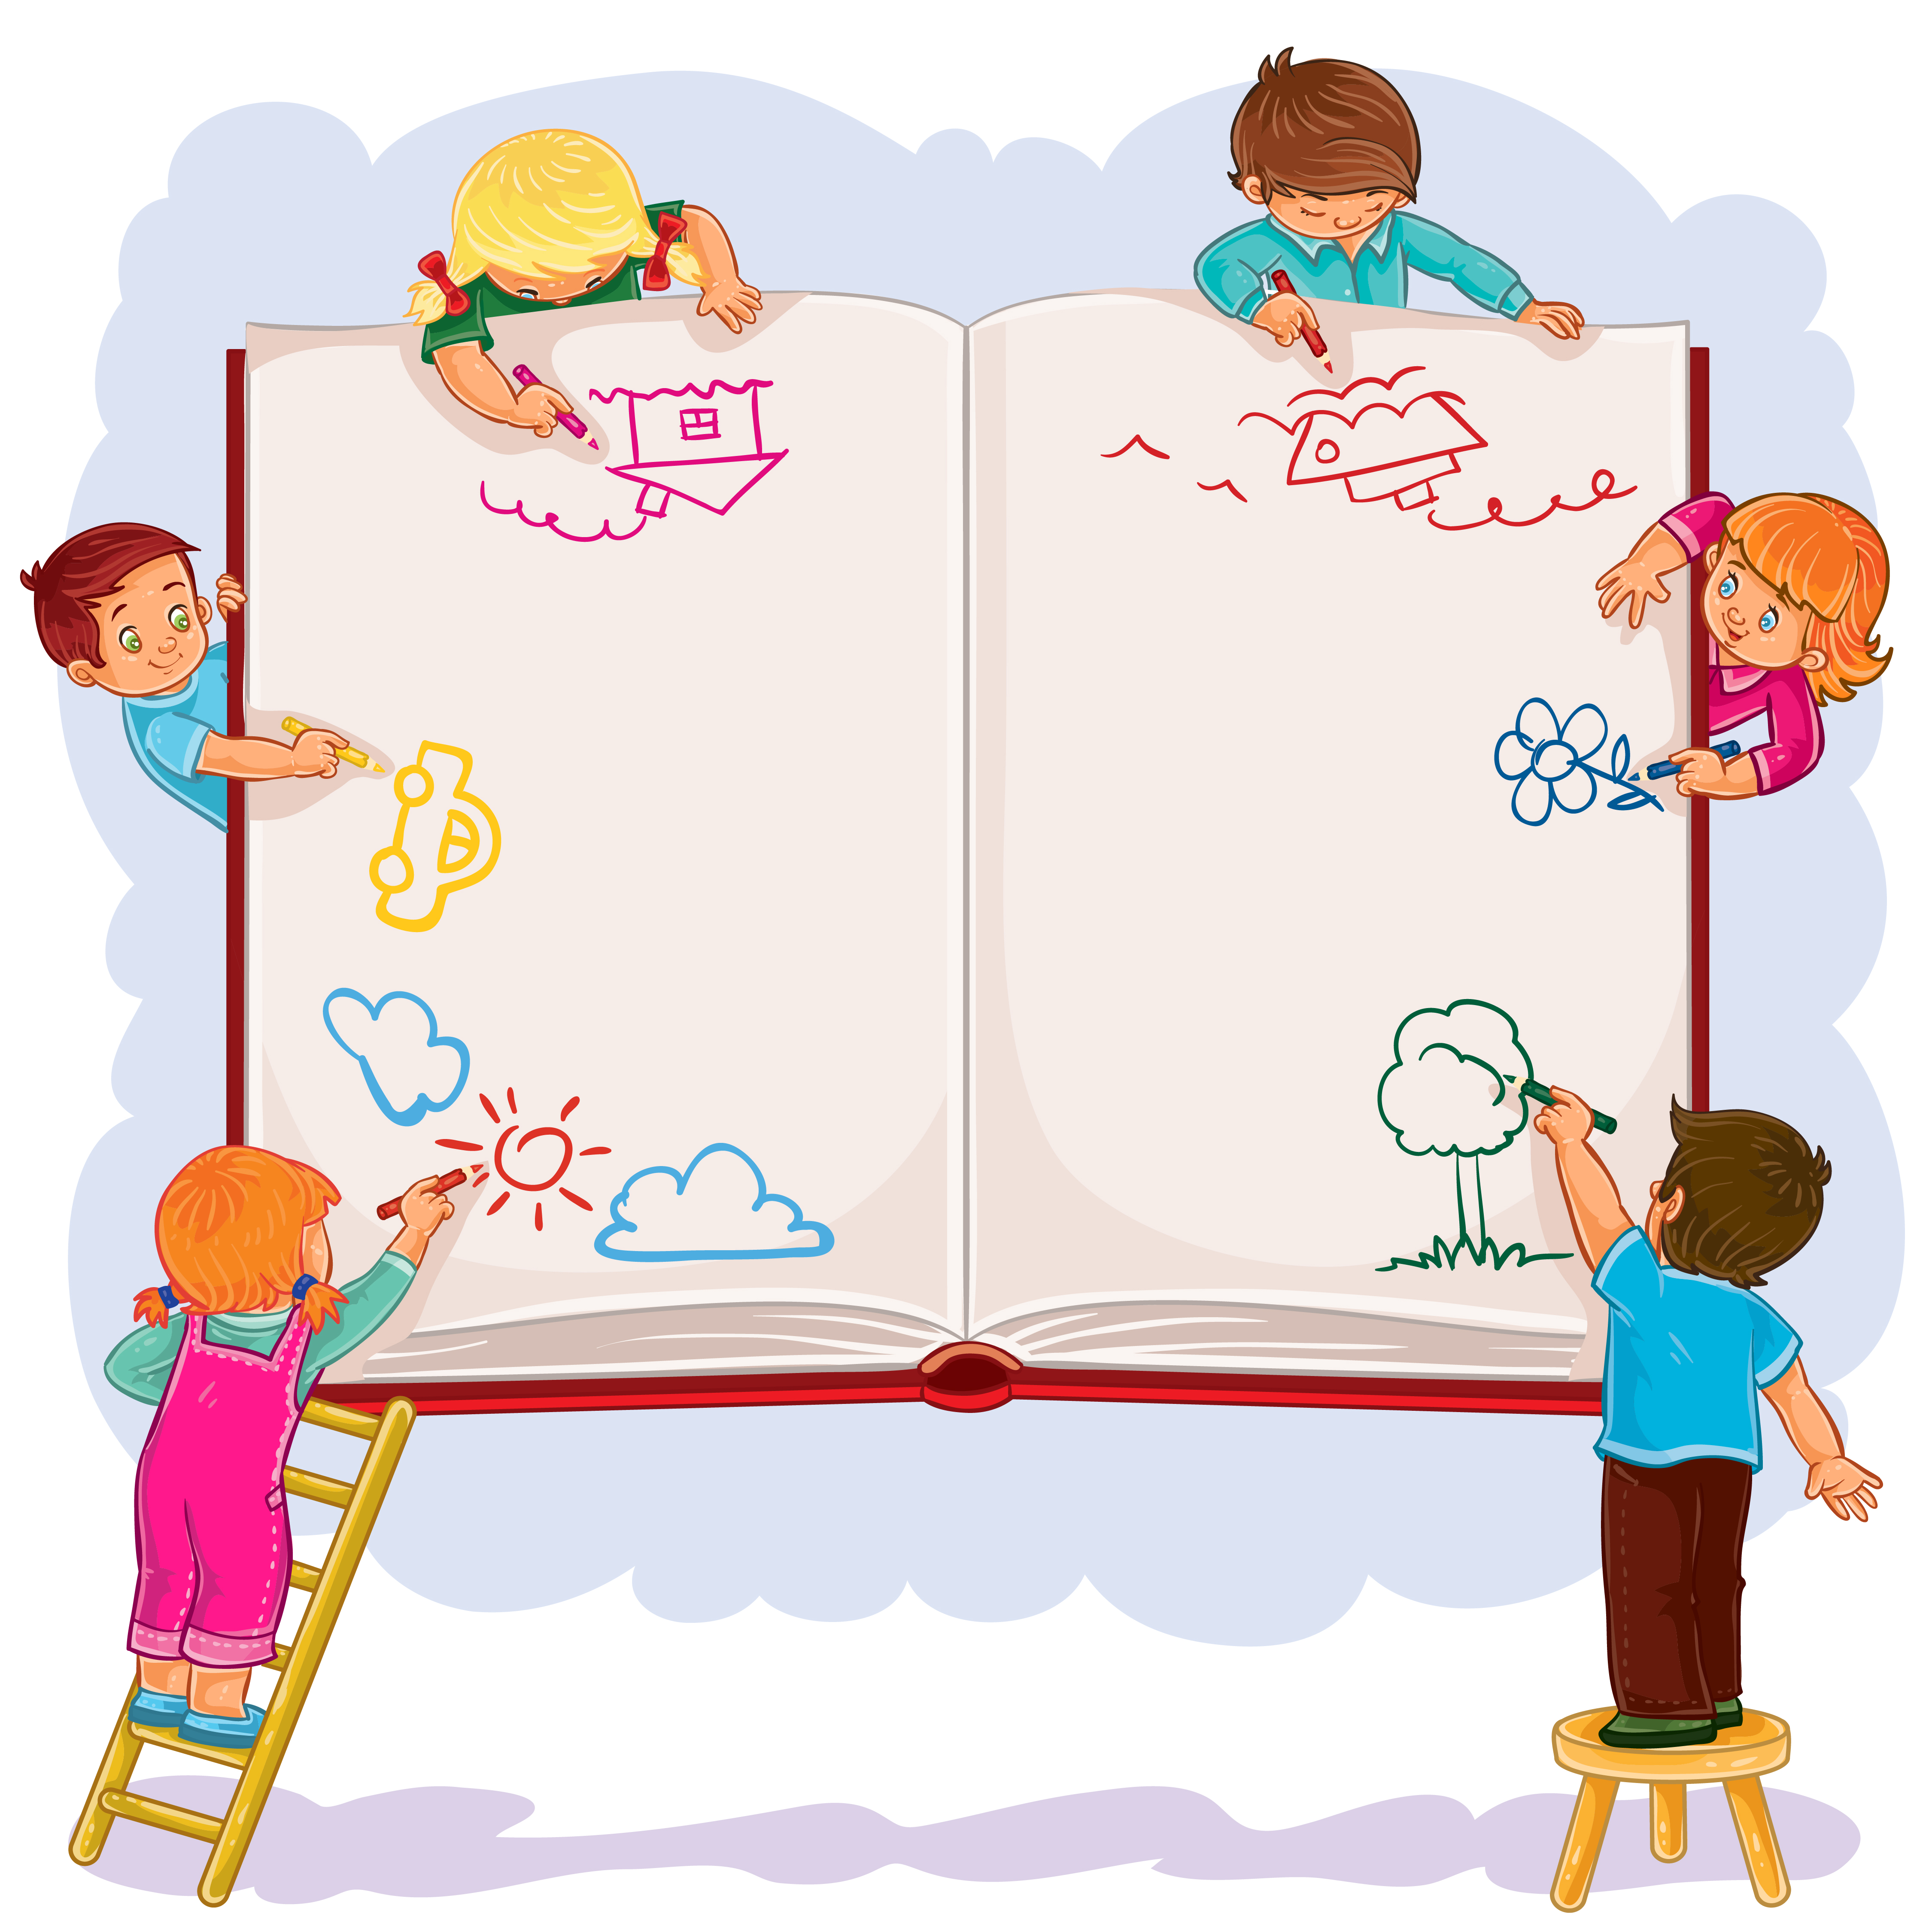
\includegraphics[width=\paperwidth,height=\paperheight]{../images/happy-children-together-draw-large-sheet-book.jpg}
      }%
  }
  \BgThispage
  
  \begin{center}
    \huge
    Tabuada de Adição
  \end{center}

  \large
  \vspace{40pt}
  \noindent
  Registre o tempo gasto (em minutos):
  \begin{table}[!htpb]
    \begin{tabular}{|c|c|c|c|c|}
      \hline
      
    \begin{tabular}{ccccc}
1 & + & 4 & = & \\
    1 & + & 2 & = & \\
    1 & + & 7 & = & \\
    1 & + & 3 & = & \\
    1 & + & 6 & = & \\
    1 & + & 8 & = & \\
    1 & + & 10 & = & \\
    1 & + & 1 & = & \\
    1 & + & 5 & = & \\
    1 & + & 9 & = &
\end{tabular}&
    \begin{tabular}{ccccc}
2 & + & 3 & = & \\
    2 & + & 1 & = & \\
    2 & + & 2 & = & \\
    2 & + & 4 & = & \\
    2 & + & 7 & = & \\
    2 & + & 5 & = & \\
    2 & + & 8 & = & \\
    2 & + & 6 & = & \\
    2 & + & 9 & = & \\
    2 & + & 10 & = &
\end{tabular}&
    \begin{tabular}{ccccc}
3 & + & 1 & = & \\
    3 & + & 4 & = & \\
    3 & + & 10 & = & \\
    3 & + & 8 & = & \\
    3 & + & 2 & = & \\
    3 & + & 3 & = & \\
    3 & + & 5 & = & \\
    3 & + & 6 & = & \\
    3 & + & 7 & = & \\
    3 & + & 9 & = &
\end{tabular}&
    \begin{tabular}{ccccc}
4 & + & 9 & = & \\
    4 & + & 2 & = & \\
    4 & + & 8 & = & \\
    4 & + & 7 & = & \\
    4 & + & 5 & = & \\
    4 & + & 10 & = & \\
    4 & + & 1 & = & \\
    4 & + & 6 & = & \\
    4 & + & 4 & = & \\
    4 & + & 3 & = &
\end{tabular}&
    \begin{tabular}{ccccc}
5 & + & 6 & = & \\
    5 & + & 2 & = & \\
    5 & + & 4 & = & \\
    5 & + & 5 & = & \\
    5 & + & 1 & = & \\
    5 & + & 7 & = & \\
    5 & + & 3 & = & \\
    5 & + & 9 & = & \\
    5 & + & 8 & = & \\
    5 & + & 10 & = &
\end{tabular}
\\ \hline
    \begin{tabular}{ccccc}
6 & + & 10 & = & \\
    6 & + & 6 & = & \\
    6 & + & 8 & = & \\
    6 & + & 4 & = & \\
    6 & + & 2 & = & \\
    6 & + & 1 & = & \\
    6 & + & 3 & = & \\
    6 & + & 7 & = & \\
    6 & + & 5 & = & \\
    6 & + & 9 & = &
\end{tabular}&
    \begin{tabular}{ccccc}
7 & + & 9 & = & \\
    7 & + & 5 & = & \\
    7 & + & 3 & = & \\
    7 & + & 10 & = & \\
    7 & + & 6 & = & \\
    7 & + & 4 & = & \\
    7 & + & 2 & = & \\
    7 & + & 8 & = & \\
    7 & + & 1 & = & \\
    7 & + & 7 & = &
\end{tabular}&
    \begin{tabular}{ccccc}
8 & + & 6 & = & \\
    8 & + & 4 & = & \\
    8 & + & 2 & = & \\
    8 & + & 10 & = & \\
    8 & + & 5 & = & \\
    8 & + & 3 & = & \\
    8 & + & 1 & = & \\
    8 & + & 7 & = & \\
    8 & + & 8 & = & \\
    8 & + & 9 & = &
\end{tabular}&
    \begin{tabular}{ccccc}
9 & + & 1 & = & \\
    9 & + & 7 & = & \\
    9 & + & 8 & = & \\
    9 & + & 6 & = & \\
    9 & + & 4 & = & \\
    9 & + & 10 & = & \\
    9 & + & 5 & = & \\
    9 & + & 3 & = & \\
    9 & + & 9 & = & \\
    9 & + & 2 & = &
\end{tabular}&
    \begin{tabular}{ccccc}
10 & + & 2 & = & \\
    10 & + & 5 & = & \\
    10 & + & 9 & = & \\
    10 & + & 10 & = & \\
    10 & + & 1 & = & \\
    10 & + & 6 & = & \\
    10 & + & 3 & = & \\
    10 & + & 4 & = & \\
    10 & + & 8 & = & \\
    10 & + & 7 & = &
\end{tabular}
      \\ \hline
    \end{tabular}
  \end{table}
  \vfil
  \begin{flushright}
    \begin{minipage}[b]{6cm}
      A tabuada é o objeto de estudo mais importante na Matemática. É o caminho para se chegar ao universo dos números. (José Carlos dos Santos)
    \end{minipage}
  \end{flushright}

  \newpage
  

  \backgroundsetup{
    scale=1,
    color=black,
    opacity=0.2,
    angle=0,
    contents={%
        \includegraphics[width=\paperwidth,height=\paperheight]{../images/jesus-children-white-background.jpg}
      }%
  }
  \BgThispage
  
  \begin{center}
    \huge
    Tabuada de Adição
  \end{center}

  \large
  \vspace{40pt}
  \noindent
  Registre o tempo gasto (em minutos):
  \begin{table}[!htpb]
    \begin{tabular}{|c|c|c|c|c|}
      \hline
      
    \begin{tabular}{ccccc}
1 & + & 7 & = & \\
    1 & + & 1 & = & \\
    1 & + & 5 & = & \\
    1 & + & 8 & = & \\
    1 & + & 9 & = & \\
    1 & + & 10 & = & \\
    1 & + & 4 & = & \\
    1 & + & 2 & = & \\
    1 & + & 3 & = & \\
    1 & + & 6 & = &
\end{tabular}&
    \begin{tabular}{ccccc}
2 & + & 4 & = & \\
    2 & + & 5 & = & \\
    2 & + & 7 & = & \\
    2 & + & 8 & = & \\
    2 & + & 6 & = & \\
    2 & + & 3 & = & \\
    2 & + & 2 & = & \\
    2 & + & 9 & = & \\
    2 & + & 1 & = & \\
    2 & + & 10 & = &
\end{tabular}&
    \begin{tabular}{ccccc}
3 & + & 7 & = & \\
    3 & + & 2 & = & \\
    3 & + & 3 & = & \\
    3 & + & 9 & = & \\
    3 & + & 5 & = & \\
    3 & + & 1 & = & \\
    3 & + & 10 & = & \\
    3 & + & 4 & = & \\
    3 & + & 6 & = & \\
    3 & + & 8 & = &
\end{tabular}&
    \begin{tabular}{ccccc}
4 & + & 2 & = & \\
    4 & + & 6 & = & \\
    4 & + & 8 & = & \\
    4 & + & 4 & = & \\
    4 & + & 3 & = & \\
    4 & + & 9 & = & \\
    4 & + & 1 & = & \\
    4 & + & 7 & = & \\
    4 & + & 10 & = & \\
    4 & + & 5 & = &
\end{tabular}&
    \begin{tabular}{ccccc}
5 & + & 1 & = & \\
    5 & + & 9 & = & \\
    5 & + & 5 & = & \\
    5 & + & 8 & = & \\
    5 & + & 3 & = & \\
    5 & + & 7 & = & \\
    5 & + & 2 & = & \\
    5 & + & 4 & = & \\
    5 & + & 6 & = & \\
    5 & + & 10 & = &
\end{tabular}
\\ \hline
    \begin{tabular}{ccccc}
6 & + & 5 & = & \\
    6 & + & 9 & = & \\
    6 & + & 8 & = & \\
    6 & + & 3 & = & \\
    6 & + & 2 & = & \\
    6 & + & 4 & = & \\
    6 & + & 7 & = & \\
    6 & + & 10 & = & \\
    6 & + & 6 & = & \\
    6 & + & 1 & = &
\end{tabular}&
    \begin{tabular}{ccccc}
7 & + & 4 & = & \\
    7 & + & 8 & = & \\
    7 & + & 7 & = & \\
    7 & + & 1 & = & \\
    7 & + & 5 & = & \\
    7 & + & 6 & = & \\
    7 & + & 9 & = & \\
    7 & + & 3 & = & \\
    7 & + & 10 & = & \\
    7 & + & 2 & = &
\end{tabular}&
    \begin{tabular}{ccccc}
8 & + & 7 & = & \\
    8 & + & 3 & = & \\
    8 & + & 4 & = & \\
    8 & + & 9 & = & \\
    8 & + & 10 & = & \\
    8 & + & 6 & = & \\
    8 & + & 8 & = & \\
    8 & + & 5 & = & \\
    8 & + & 1 & = & \\
    8 & + & 2 & = &
\end{tabular}&
    \begin{tabular}{ccccc}
9 & + & 5 & = & \\
    9 & + & 7 & = & \\
    9 & + & 3 & = & \\
    9 & + & 2 & = & \\
    9 & + & 6 & = & \\
    9 & + & 9 & = & \\
    9 & + & 4 & = & \\
    9 & + & 1 & = & \\
    9 & + & 8 & = & \\
    9 & + & 10 & = &
\end{tabular}&
    \begin{tabular}{ccccc}
10 & + & 7 & = & \\
    10 & + & 5 & = & \\
    10 & + & 9 & = & \\
    10 & + & 8 & = & \\
    10 & + & 4 & = & \\
    10 & + & 6 & = & \\
    10 & + & 1 & = & \\
    10 & + & 2 & = & \\
    10 & + & 3 & = & \\
    10 & + & 10 & = &
\end{tabular}
      \\ \hline
    \end{tabular}
  \end{table}
  \vfil
  \begin{flushright}
    \begin{minipage}[b]{6cm}
      A tabuada é o objeto de estudo mais importante na Matemática. É o caminho para se chegar ao universo dos números. (José Carlos dos Santos)
    \end{minipage}
  \end{flushright}

  \newpage
  

  \backgroundsetup{
    scale=1,
    color=black,
    opacity=0.2,
    angle=0,
    contents={%
        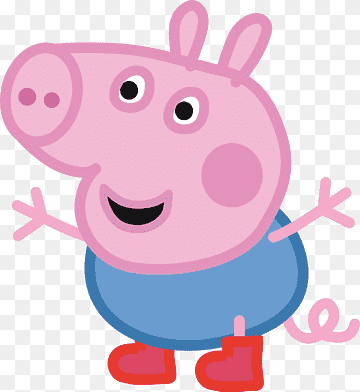
\includegraphics[width=\paperwidth,height=\paperheight]{../images/jorge.png}
      }%
  }
  \BgThispage
  
  \begin{center}
    \huge
    Tabuada de Adição
  \end{center}

  \large
  \vspace{40pt}
  \noindent
  Registre o tempo gasto (em minutos):
  \begin{table}[!htpb]
    \begin{tabular}{|c|c|c|c|c|}
      \hline
      
    \begin{tabular}{ccccc}
1 & + & 10 & = & \\
    1 & + & 7 & = & \\
    1 & + & 9 & = & \\
    1 & + & 8 & = & \\
    1 & + & 4 & = & \\
    1 & + & 6 & = & \\
    1 & + & 3 & = & \\
    1 & + & 1 & = & \\
    1 & + & 5 & = & \\
    1 & + & 2 & = &
\end{tabular}&
    \begin{tabular}{ccccc}
2 & + & 3 & = & \\
    2 & + & 5 & = & \\
    2 & + & 1 & = & \\
    2 & + & 7 & = & \\
    2 & + & 10 & = & \\
    2 & + & 8 & = & \\
    2 & + & 6 & = & \\
    2 & + & 2 & = & \\
    2 & + & 4 & = & \\
    2 & + & 9 & = &
\end{tabular}&
    \begin{tabular}{ccccc}
3 & + & 2 & = & \\
    3 & + & 8 & = & \\
    3 & + & 7 & = & \\
    3 & + & 4 & = & \\
    3 & + & 1 & = & \\
    3 & + & 6 & = & \\
    3 & + & 5 & = & \\
    3 & + & 9 & = & \\
    3 & + & 10 & = & \\
    3 & + & 3 & = &
\end{tabular}&
    \begin{tabular}{ccccc}
4 & + & 8 & = & \\
    4 & + & 2 & = & \\
    4 & + & 10 & = & \\
    4 & + & 1 & = & \\
    4 & + & 6 & = & \\
    4 & + & 9 & = & \\
    4 & + & 4 & = & \\
    4 & + & 5 & = & \\
    4 & + & 3 & = & \\
    4 & + & 7 & = &
\end{tabular}&
    \begin{tabular}{ccccc}
5 & + & 1 & = & \\
    5 & + & 8 & = & \\
    5 & + & 5 & = & \\
    5 & + & 3 & = & \\
    5 & + & 7 & = & \\
    5 & + & 9 & = & \\
    5 & + & 10 & = & \\
    5 & + & 2 & = & \\
    5 & + & 4 & = & \\
    5 & + & 6 & = &
\end{tabular}
\\ \hline
    \begin{tabular}{ccccc}
6 & + & 4 & = & \\
    6 & + & 7 & = & \\
    6 & + & 3 & = & \\
    6 & + & 5 & = & \\
    6 & + & 8 & = & \\
    6 & + & 9 & = & \\
    6 & + & 2 & = & \\
    6 & + & 10 & = & \\
    6 & + & 1 & = & \\
    6 & + & 6 & = &
\end{tabular}&
    \begin{tabular}{ccccc}
7 & + & 2 & = & \\
    7 & + & 1 & = & \\
    7 & + & 4 & = & \\
    7 & + & 7 & = & \\
    7 & + & 8 & = & \\
    7 & + & 3 & = & \\
    7 & + & 10 & = & \\
    7 & + & 5 & = & \\
    7 & + & 9 & = & \\
    7 & + & 6 & = &
\end{tabular}&
    \begin{tabular}{ccccc}
8 & + & 4 & = & \\
    8 & + & 3 & = & \\
    8 & + & 5 & = & \\
    8 & + & 1 & = & \\
    8 & + & 9 & = & \\
    8 & + & 2 & = & \\
    8 & + & 8 & = & \\
    8 & + & 10 & = & \\
    8 & + & 6 & = & \\
    8 & + & 7 & = &
\end{tabular}&
    \begin{tabular}{ccccc}
9 & + & 3 & = & \\
    9 & + & 9 & = & \\
    9 & + & 8 & = & \\
    9 & + & 4 & = & \\
    9 & + & 1 & = & \\
    9 & + & 5 & = & \\
    9 & + & 2 & = & \\
    9 & + & 7 & = & \\
    9 & + & 6 & = & \\
    9 & + & 10 & = &
\end{tabular}&
    \begin{tabular}{ccccc}
10 & + & 8 & = & \\
    10 & + & 9 & = & \\
    10 & + & 2 & = & \\
    10 & + & 5 & = & \\
    10 & + & 1 & = & \\
    10 & + & 3 & = & \\
    10 & + & 6 & = & \\
    10 & + & 10 & = & \\
    10 & + & 7 & = & \\
    10 & + & 4 & = &
\end{tabular}
      \\ \hline
    \end{tabular}
  \end{table}
  \vfil
  \begin{flushright}
    \begin{minipage}[b]{6cm}
      A tabuada é o objeto de estudo mais importante na Matemática. É o caminho para se chegar ao universo dos números. (José Carlos dos Santos)
    \end{minipage}
  \end{flushright}

  \newpage
  

  \backgroundsetup{
    scale=1,
    color=black,
    opacity=0.2,
    angle=0,
    contents={%
        
\includegraphics[width=\paperwidth,height=\paperheight]{../images/monkey-kings.jpg}
      }%
  }
  \BgThispage
  
  \begin{center}
    \huge
    Tabuada de Adição
  \end{center}

  \large
  \vspace{40pt}
  \noindent
  Registre o tempo gasto (em minutos):
  \begin{table}[!htpb]
    \begin{tabular}{|c|c|c|c|c|}
      \hline
      
    \begin{tabular}{ccccc}
1 & + & 7 & = & \\
    1 & + & 4 & = & \\
    1 & + & 8 & = & \\
    1 & + & 5 & = & \\
    1 & + & 1 & = & \\
    1 & + & 9 & = & \\
    1 & + & 6 & = & \\
    1 & + & 2 & = & \\
    1 & + & 3 & = & \\
    1 & + & 10 & = &
\end{tabular}&
    \begin{tabular}{ccccc}
2 & + & 2 & = & \\
    2 & + & 6 & = & \\
    2 & + & 1 & = & \\
    2 & + & 10 & = & \\
    2 & + & 3 & = & \\
    2 & + & 5 & = & \\
    2 & + & 8 & = & \\
    2 & + & 4 & = & \\
    2 & + & 7 & = & \\
    2 & + & 9 & = &
\end{tabular}&
    \begin{tabular}{ccccc}
3 & + & 6 & = & \\
    3 & + & 1 & = & \\
    3 & + & 2 & = & \\
    3 & + & 4 & = & \\
    3 & + & 8 & = & \\
    3 & + & 10 & = & \\
    3 & + & 5 & = & \\
    3 & + & 3 & = & \\
    3 & + & 7 & = & \\
    3 & + & 9 & = &
\end{tabular}&
    \begin{tabular}{ccccc}
4 & + & 4 & = & \\
    4 & + & 1 & = & \\
    4 & + & 6 & = & \\
    4 & + & 8 & = & \\
    4 & + & 9 & = & \\
    4 & + & 5 & = & \\
    4 & + & 10 & = & \\
    4 & + & 2 & = & \\
    4 & + & 3 & = & \\
    4 & + & 7 & = &
\end{tabular}&
    \begin{tabular}{ccccc}
5 & + & 9 & = & \\
    5 & + & 7 & = & \\
    5 & + & 8 & = & \\
    5 & + & 5 & = & \\
    5 & + & 4 & = & \\
    5 & + & 10 & = & \\
    5 & + & 1 & = & \\
    5 & + & 3 & = & \\
    5 & + & 6 & = & \\
    5 & + & 2 & = &
\end{tabular}
\\ \hline
    \begin{tabular}{ccccc}
6 & + & 4 & = & \\
    6 & + & 2 & = & \\
    6 & + & 7 & = & \\
    6 & + & 3 & = & \\
    6 & + & 10 & = & \\
    6 & + & 6 & = & \\
    6 & + & 8 & = & \\
    6 & + & 9 & = & \\
    6 & + & 5 & = & \\
    6 & + & 1 & = &
\end{tabular}&
    \begin{tabular}{ccccc}
7 & + & 4 & = & \\
    7 & + & 8 & = & \\
    7 & + & 3 & = & \\
    7 & + & 10 & = & \\
    7 & + & 9 & = & \\
    7 & + & 2 & = & \\
    7 & + & 1 & = & \\
    7 & + & 7 & = & \\
    7 & + & 6 & = & \\
    7 & + & 5 & = &
\end{tabular}&
    \begin{tabular}{ccccc}
8 & + & 9 & = & \\
    8 & + & 10 & = & \\
    8 & + & 1 & = & \\
    8 & + & 7 & = & \\
    8 & + & 2 & = & \\
    8 & + & 4 & = & \\
    8 & + & 3 & = & \\
    8 & + & 5 & = & \\
    8 & + & 8 & = & \\
    8 & + & 6 & = &
\end{tabular}&
    \begin{tabular}{ccccc}
9 & + & 6 & = & \\
    9 & + & 9 & = & \\
    9 & + & 7 & = & \\
    9 & + & 5 & = & \\
    9 & + & 3 & = & \\
    9 & + & 10 & = & \\
    9 & + & 1 & = & \\
    9 & + & 2 & = & \\
    9 & + & 4 & = & \\
    9 & + & 8 & = &
\end{tabular}&
    \begin{tabular}{ccccc}
10 & + & 7 & = & \\
    10 & + & 2 & = & \\
    10 & + & 4 & = & \\
    10 & + & 9 & = & \\
    10 & + & 10 & = & \\
    10 & + & 6 & = & \\
    10 & + & 3 & = & \\
    10 & + & 8 & = & \\
    10 & + & 1 & = & \\
    10 & + & 5 & = &
\end{tabular}
      \\ \hline
    \end{tabular}
  \end{table}
  \vfil
  \begin{flushright}
    \begin{minipage}[b]{6cm}
      A tabuada é o objeto de estudo mais importante na Matemática. É o caminho para se chegar ao universo dos números. (José Carlos dos Santos)
    \end{minipage}
  \end{flushright}

  \newpage
  

  \backgroundsetup{
    scale=1,
    color=black,
    opacity=0.2,
    angle=0,
    contents={%
        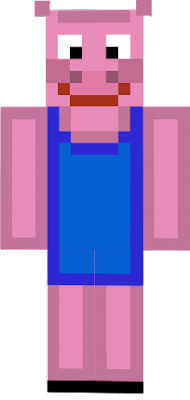
\includegraphics[width=\paperwidth,height=\paperheight]{../images/pepa.png}
      }%
  }
  \BgThispage
  
  \begin{center}
    \huge
    Tabuada de Adição
  \end{center}

  \large
  \vspace{40pt}
  \noindent
  Registre o tempo gasto (em minutos):
  \begin{table}[!htpb]
    \begin{tabular}{|c|c|c|c|c|}
      \hline
      
    \begin{tabular}{ccccc}
1 & + & 7 & = & \\
    1 & + & 3 & = & \\
    1 & + & 10 & = & \\
    1 & + & 8 & = & \\
    1 & + & 5 & = & \\
    1 & + & 9 & = & \\
    1 & + & 2 & = & \\
    1 & + & 6 & = & \\
    1 & + & 1 & = & \\
    1 & + & 4 & = &
\end{tabular}&
    \begin{tabular}{ccccc}
2 & + & 1 & = & \\
    2 & + & 6 & = & \\
    2 & + & 4 & = & \\
    2 & + & 2 & = & \\
    2 & + & 10 & = & \\
    2 & + & 7 & = & \\
    2 & + & 3 & = & \\
    2 & + & 9 & = & \\
    2 & + & 8 & = & \\
    2 & + & 5 & = &
\end{tabular}&
    \begin{tabular}{ccccc}
3 & + & 6 & = & \\
    3 & + & 7 & = & \\
    3 & + & 5 & = & \\
    3 & + & 2 & = & \\
    3 & + & 4 & = & \\
    3 & + & 3 & = & \\
    3 & + & 8 & = & \\
    3 & + & 1 & = & \\
    3 & + & 10 & = & \\
    3 & + & 9 & = &
\end{tabular}&
    \begin{tabular}{ccccc}
4 & + & 5 & = & \\
    4 & + & 10 & = & \\
    4 & + & 1 & = & \\
    4 & + & 2 & = & \\
    4 & + & 6 & = & \\
    4 & + & 8 & = & \\
    4 & + & 7 & = & \\
    4 & + & 9 & = & \\
    4 & + & 4 & = & \\
    4 & + & 3 & = &
\end{tabular}&
    \begin{tabular}{ccccc}
5 & + & 4 & = & \\
    5 & + & 10 & = & \\
    5 & + & 2 & = & \\
    5 & + & 9 & = & \\
    5 & + & 6 & = & \\
    5 & + & 8 & = & \\
    5 & + & 3 & = & \\
    5 & + & 7 & = & \\
    5 & + & 5 & = & \\
    5 & + & 1 & = &
\end{tabular}
\\ \hline
    \begin{tabular}{ccccc}
6 & + & 5 & = & \\
    6 & + & 9 & = & \\
    6 & + & 7 & = & \\
    6 & + & 4 & = & \\
    6 & + & 8 & = & \\
    6 & + & 1 & = & \\
    6 & + & 10 & = & \\
    6 & + & 6 & = & \\
    6 & + & 3 & = & \\
    6 & + & 2 & = &
\end{tabular}&
    \begin{tabular}{ccccc}
7 & + & 6 & = & \\
    7 & + & 10 & = & \\
    7 & + & 9 & = & \\
    7 & + & 1 & = & \\
    7 & + & 3 & = & \\
    7 & + & 4 & = & \\
    7 & + & 2 & = & \\
    7 & + & 5 & = & \\
    7 & + & 7 & = & \\
    7 & + & 8 & = &
\end{tabular}&
    \begin{tabular}{ccccc}
8 & + & 5 & = & \\
    8 & + & 7 & = & \\
    8 & + & 3 & = & \\
    8 & + & 1 & = & \\
    8 & + & 4 & = & \\
    8 & + & 10 & = & \\
    8 & + & 8 & = & \\
    8 & + & 9 & = & \\
    8 & + & 6 & = & \\
    8 & + & 2 & = &
\end{tabular}&
    \begin{tabular}{ccccc}
9 & + & 10 & = & \\
    9 & + & 9 & = & \\
    9 & + & 3 & = & \\
    9 & + & 1 & = & \\
    9 & + & 4 & = & \\
    9 & + & 8 & = & \\
    9 & + & 5 & = & \\
    9 & + & 6 & = & \\
    9 & + & 7 & = & \\
    9 & + & 2 & = &
\end{tabular}&
    \begin{tabular}{ccccc}
10 & + & 7 & = & \\
    10 & + & 10 & = & \\
    10 & + & 3 & = & \\
    10 & + & 5 & = & \\
    10 & + & 4 & = & \\
    10 & + & 6 & = & \\
    10 & + & 9 & = & \\
    10 & + & 2 & = & \\
    10 & + & 1 & = & \\
    10 & + & 8 & = &
\end{tabular}
      \\ \hline
    \end{tabular}
  \end{table}
  \vfil
  \begin{flushright}
    \begin{minipage}[b]{6cm}
      A tabuada é o objeto de estudo mais importante na Matemática. É o caminho para se chegar ao universo dos números. (José Carlos dos Santos)
    \end{minipage}
  \end{flushright}

  \newpage
  

  \backgroundsetup{
    scale=1,
    color=black,
    opacity=0.2,
    angle=0,
    contents={%
        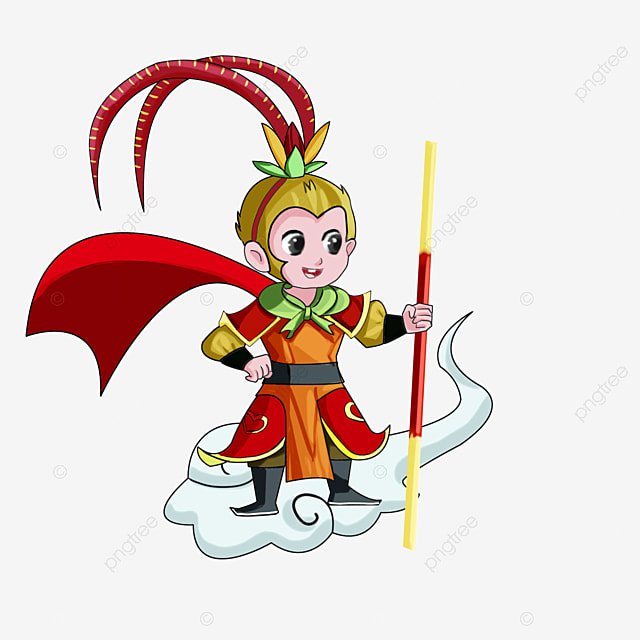
\includegraphics[width=\paperwidth,height=\paperheight]{../images/rei-macaco.jpg}
      }%
  }
  \BgThispage
  
  \begin{center}
    \huge
    Tabuada de Adição
  \end{center}

  \large
  \vspace{40pt}
  \noindent
  Registre o tempo gasto (em minutos):
  \begin{table}[!htpb]
    \begin{tabular}{|c|c|c|c|c|}
      \hline
      
    \begin{tabular}{ccccc}
1 & + & 7 & = & \\
    1 & + & 9 & = & \\
    1 & + & 1 & = & \\
    1 & + & 8 & = & \\
    1 & + & 4 & = & \\
    1 & + & 5 & = & \\
    1 & + & 3 & = & \\
    1 & + & 10 & = & \\
    1 & + & 2 & = & \\
    1 & + & 6 & = &
\end{tabular}&
    \begin{tabular}{ccccc}
2 & + & 8 & = & \\
    2 & + & 5 & = & \\
    2 & + & 4 & = & \\
    2 & + & 10 & = & \\
    2 & + & 2 & = & \\
    2 & + & 7 & = & \\
    2 & + & 1 & = & \\
    2 & + & 9 & = & \\
    2 & + & 3 & = & \\
    2 & + & 6 & = &
\end{tabular}&
    \begin{tabular}{ccccc}
3 & + & 7 & = & \\
    3 & + & 1 & = & \\
    3 & + & 2 & = & \\
    3 & + & 6 & = & \\
    3 & + & 5 & = & \\
    3 & + & 4 & = & \\
    3 & + & 9 & = & \\
    3 & + & 10 & = & \\
    3 & + & 8 & = & \\
    3 & + & 3 & = &
\end{tabular}&
    \begin{tabular}{ccccc}
4 & + & 5 & = & \\
    4 & + & 8 & = & \\
    4 & + & 4 & = & \\
    4 & + & 10 & = & \\
    4 & + & 9 & = & \\
    4 & + & 7 & = & \\
    4 & + & 1 & = & \\
    4 & + & 6 & = & \\
    4 & + & 2 & = & \\
    4 & + & 3 & = &
\end{tabular}&
    \begin{tabular}{ccccc}
5 & + & 5 & = & \\
    5 & + & 8 & = & \\
    5 & + & 2 & = & \\
    5 & + & 3 & = & \\
    5 & + & 7 & = & \\
    5 & + & 6 & = & \\
    5 & + & 9 & = & \\
    5 & + & 4 & = & \\
    5 & + & 10 & = & \\
    5 & + & 1 & = &
\end{tabular}
\\ \hline
    \begin{tabular}{ccccc}
6 & + & 9 & = & \\
    6 & + & 10 & = & \\
    6 & + & 8 & = & \\
    6 & + & 3 & = & \\
    6 & + & 7 & = & \\
    6 & + & 4 & = & \\
    6 & + & 2 & = & \\
    6 & + & 1 & = & \\
    6 & + & 5 & = & \\
    6 & + & 6 & = &
\end{tabular}&
    \begin{tabular}{ccccc}
7 & + & 5 & = & \\
    7 & + & 3 & = & \\
    7 & + & 9 & = & \\
    7 & + & 8 & = & \\
    7 & + & 10 & = & \\
    7 & + & 7 & = & \\
    7 & + & 6 & = & \\
    7 & + & 4 & = & \\
    7 & + & 1 & = & \\
    7 & + & 2 & = &
\end{tabular}&
    \begin{tabular}{ccccc}
8 & + & 4 & = & \\
    8 & + & 1 & = & \\
    8 & + & 2 & = & \\
    8 & + & 6 & = & \\
    8 & + & 5 & = & \\
    8 & + & 8 & = & \\
    8 & + & 10 & = & \\
    8 & + & 3 & = & \\
    8 & + & 9 & = & \\
    8 & + & 7 & = &
\end{tabular}&
    \begin{tabular}{ccccc}
9 & + & 8 & = & \\
    9 & + & 5 & = & \\
    9 & + & 3 & = & \\
    9 & + & 7 & = & \\
    9 & + & 9 & = & \\
    9 & + & 6 & = & \\
    9 & + & 10 & = & \\
    9 & + & 4 & = & \\
    9 & + & 1 & = & \\
    9 & + & 2 & = &
\end{tabular}&
    \begin{tabular}{ccccc}
10 & + & 5 & = & \\
    10 & + & 6 & = & \\
    10 & + & 3 & = & \\
    10 & + & 7 & = & \\
    10 & + & 4 & = & \\
    10 & + & 2 & = & \\
    10 & + & 8 & = & \\
    10 & + & 9 & = & \\
    10 & + & 10 & = & \\
    10 & + & 1 & = &
\end{tabular}
      \\ \hline
    \end{tabular}
  \end{table}
  \vfil
  \begin{flushright}
    \begin{minipage}[b]{6cm}
      A tabuada é o objeto de estudo mais importante na Matemática. É o caminho para se chegar ao universo dos números. (José Carlos dos Santos)
    \end{minipage}
  \end{flushright}

  \newpage
  

  \backgroundsetup{
    scale=1,
    color=black,
    opacity=0.2,
    angle=0,
    contents={%
        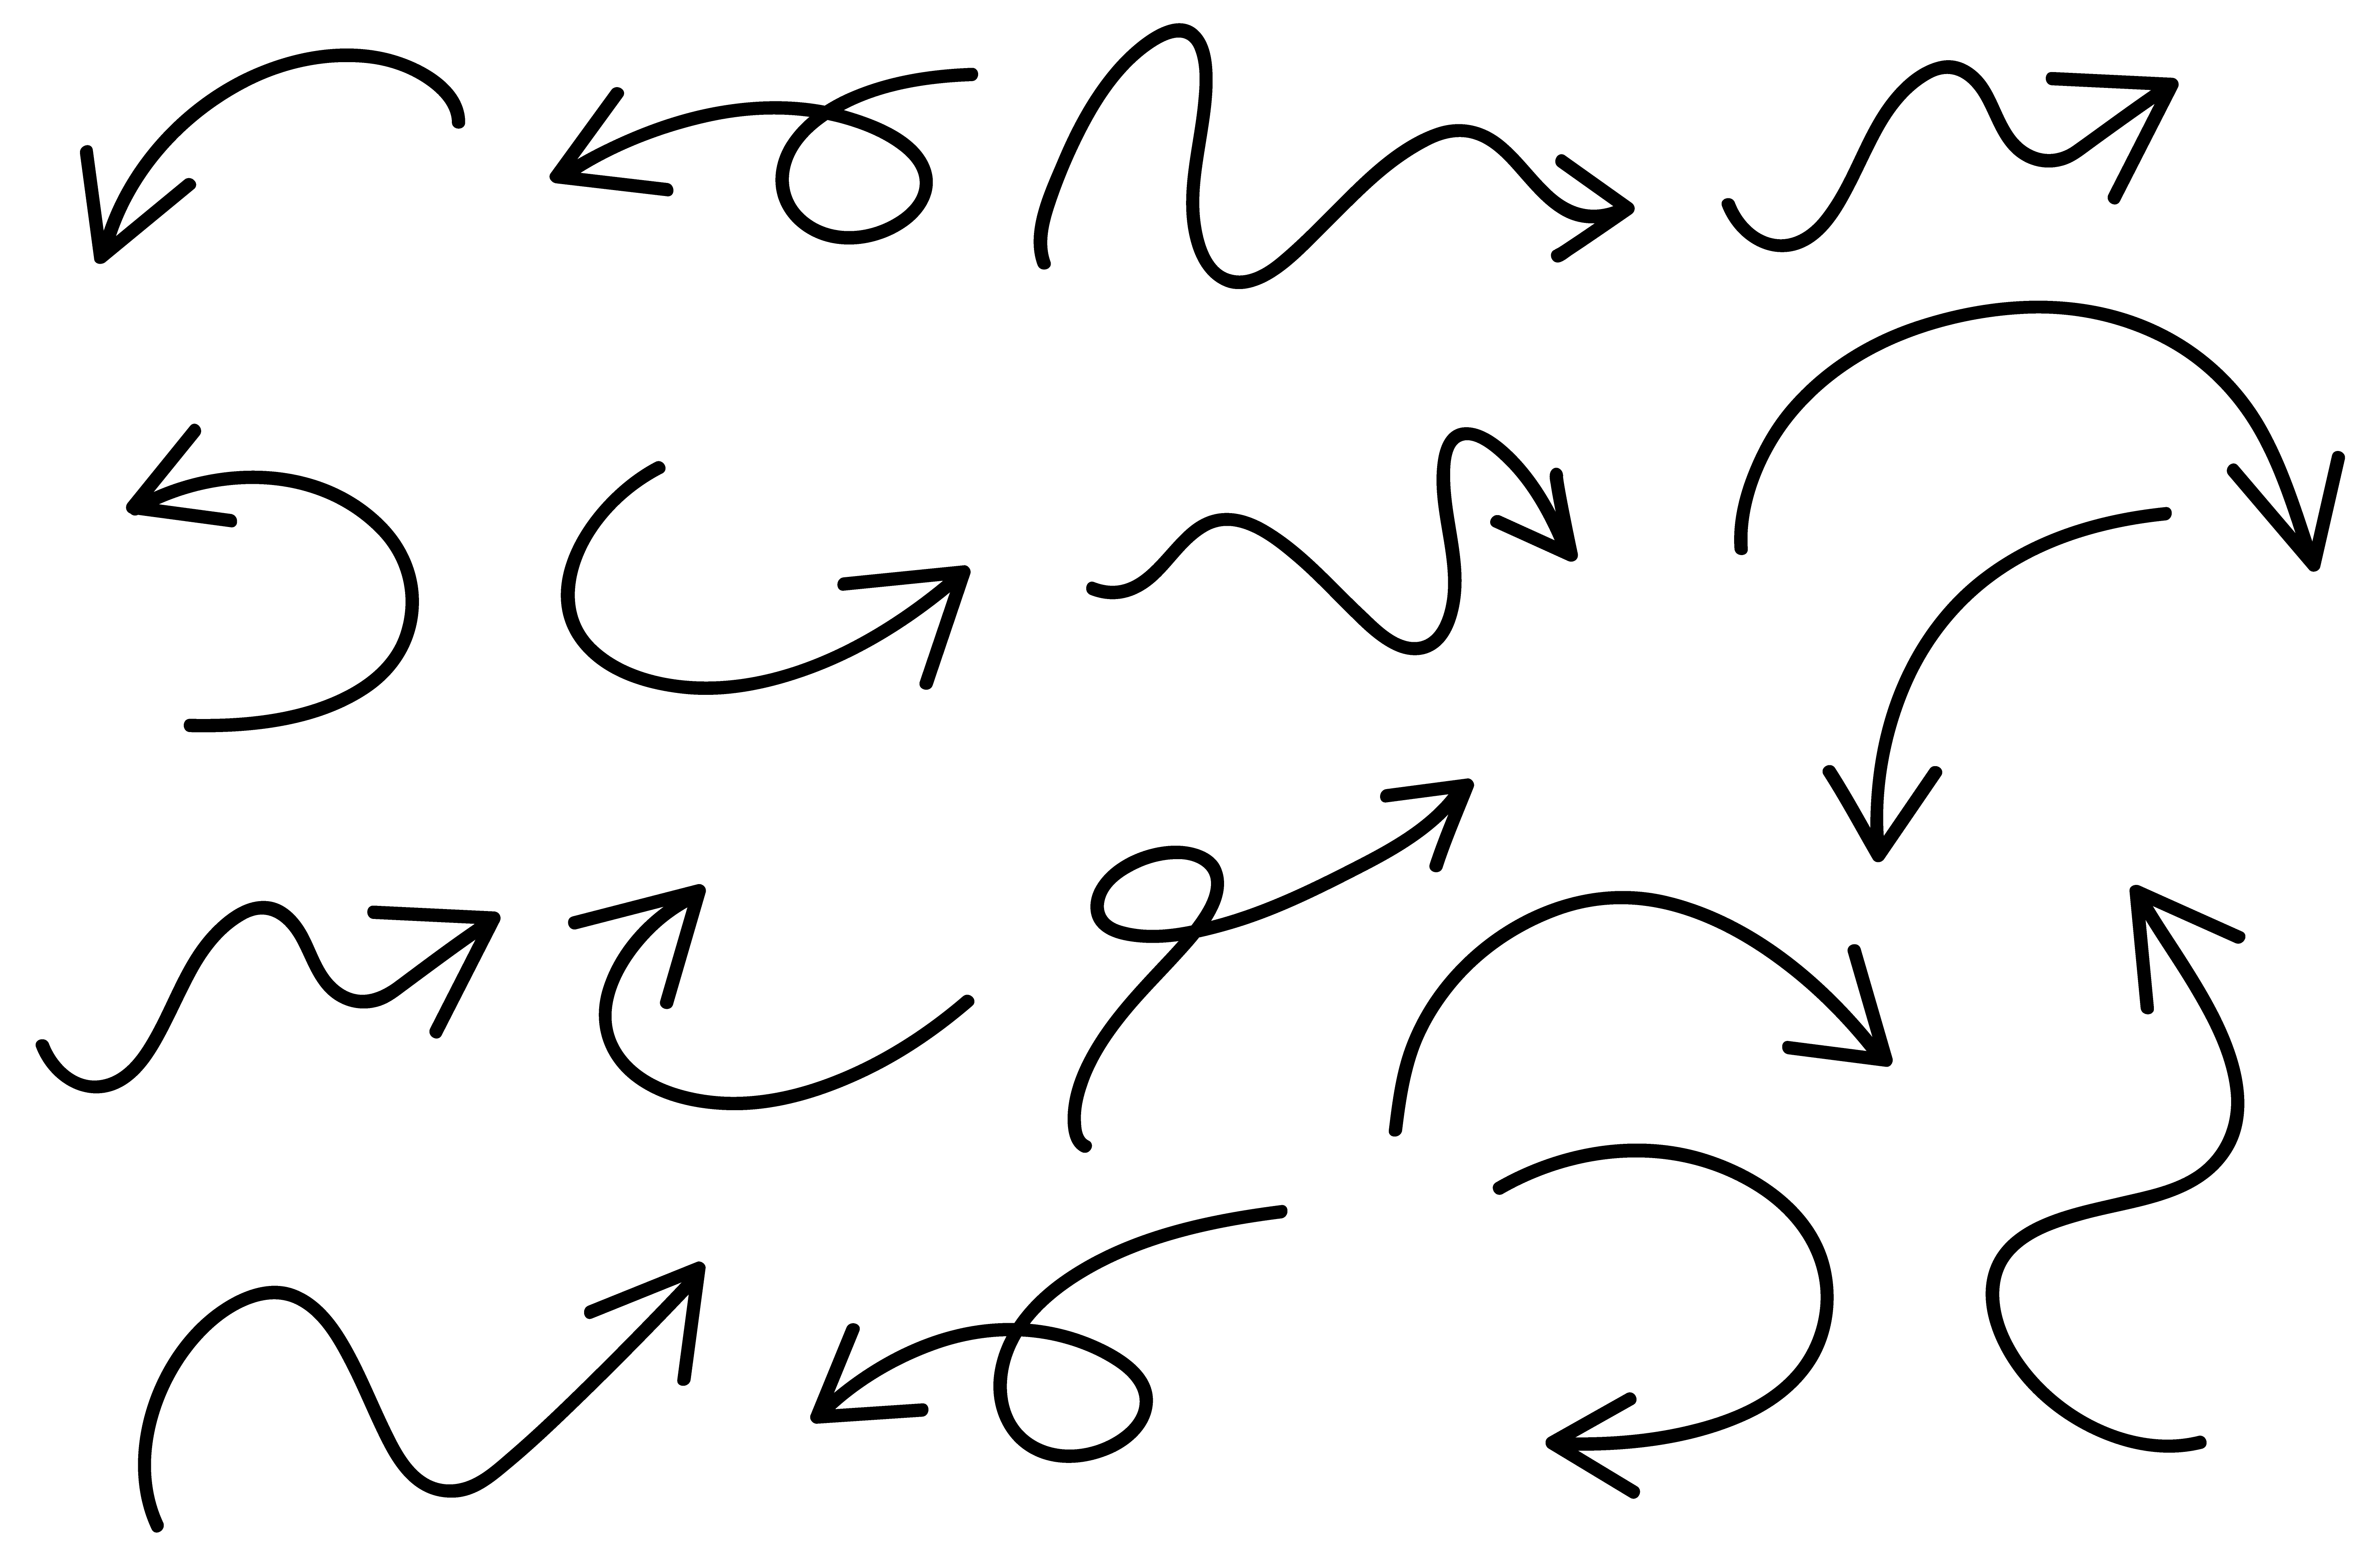
\includegraphics[width=\paperwidth,height=\paperheight]{../images/set-hand-drawn-arrow-doodles-white.jpg}
      }%
  }
  \BgThispage
  
  \begin{center}
    \huge
    Tabuada de Adição
  \end{center}

  \large
  \vspace{40pt}
  \noindent
  Registre o tempo gasto (em minutos):
  \begin{table}[!htpb]
    \begin{tabular}{|c|c|c|c|c|}
      \hline
      
    \begin{tabular}{ccccc}
1 & + & 10 & = & \\
    1 & + & 7 & = & \\
    1 & + & 6 & = & \\
    1 & + & 2 & = & \\
    1 & + & 9 & = & \\
    1 & + & 5 & = & \\
    1 & + & 8 & = & \\
    1 & + & 1 & = & \\
    1 & + & 3 & = & \\
    1 & + & 4 & = &
\end{tabular}&
    \begin{tabular}{ccccc}
2 & + & 9 & = & \\
    2 & + & 7 & = & \\
    2 & + & 2 & = & \\
    2 & + & 8 & = & \\
    2 & + & 4 & = & \\
    2 & + & 3 & = & \\
    2 & + & 6 & = & \\
    2 & + & 1 & = & \\
    2 & + & 10 & = & \\
    2 & + & 5 & = &
\end{tabular}&
    \begin{tabular}{ccccc}
3 & + & 5 & = & \\
    3 & + & 4 & = & \\
    3 & + & 8 & = & \\
    3 & + & 1 & = & \\
    3 & + & 2 & = & \\
    3 & + & 9 & = & \\
    3 & + & 7 & = & \\
    3 & + & 6 & = & \\
    3 & + & 3 & = & \\
    3 & + & 10 & = &
\end{tabular}&
    \begin{tabular}{ccccc}
4 & + & 7 & = & \\
    4 & + & 2 & = & \\
    4 & + & 8 & = & \\
    4 & + & 5 & = & \\
    4 & + & 6 & = & \\
    4 & + & 1 & = & \\
    4 & + & 9 & = & \\
    4 & + & 3 & = & \\
    4 & + & 10 & = & \\
    4 & + & 4 & = &
\end{tabular}&
    \begin{tabular}{ccccc}
5 & + & 3 & = & \\
    5 & + & 10 & = & \\
    5 & + & 5 & = & \\
    5 & + & 7 & = & \\
    5 & + & 1 & = & \\
    5 & + & 6 & = & \\
    5 & + & 4 & = & \\
    5 & + & 8 & = & \\
    5 & + & 9 & = & \\
    5 & + & 2 & = &
\end{tabular}
\\ \hline
    \begin{tabular}{ccccc}
6 & + & 10 & = & \\
    6 & + & 3 & = & \\
    6 & + & 5 & = & \\
    6 & + & 7 & = & \\
    6 & + & 9 & = & \\
    6 & + & 8 & = & \\
    6 & + & 6 & = & \\
    6 & + & 1 & = & \\
    6 & + & 4 & = & \\
    6 & + & 2 & = &
\end{tabular}&
    \begin{tabular}{ccccc}
7 & + & 7 & = & \\
    7 & + & 2 & = & \\
    7 & + & 3 & = & \\
    7 & + & 1 & = & \\
    7 & + & 6 & = & \\
    7 & + & 5 & = & \\
    7 & + & 8 & = & \\
    7 & + & 9 & = & \\
    7 & + & 10 & = & \\
    7 & + & 4 & = &
\end{tabular}&
    \begin{tabular}{ccccc}
8 & + & 1 & = & \\
    8 & + & 5 & = & \\
    8 & + & 6 & = & \\
    8 & + & 9 & = & \\
    8 & + & 8 & = & \\
    8 & + & 3 & = & \\
    8 & + & 7 & = & \\
    8 & + & 2 & = & \\
    8 & + & 4 & = & \\
    8 & + & 10 & = &
\end{tabular}&
    \begin{tabular}{ccccc}
9 & + & 3 & = & \\
    9 & + & 4 & = & \\
    9 & + & 5 & = & \\
    9 & + & 2 & = & \\
    9 & + & 10 & = & \\
    9 & + & 7 & = & \\
    9 & + & 6 & = & \\
    9 & + & 8 & = & \\
    9 & + & 1 & = & \\
    9 & + & 9 & = &
\end{tabular}&
    \begin{tabular}{ccccc}
10 & + & 7 & = & \\
    10 & + & 6 & = & \\
    10 & + & 10 & = & \\
    10 & + & 4 & = & \\
    10 & + & 3 & = & \\
    10 & + & 9 & = & \\
    10 & + & 2 & = & \\
    10 & + & 8 & = & \\
    10 & + & 5 & = & \\
    10 & + & 1 & = &
\end{tabular}
      \\ \hline
    \end{tabular}
  \end{table}
  \vfil
  \begin{flushright}
    \begin{minipage}[b]{6cm}
      A tabuada é o objeto de estudo mais importante na Matemática. É o caminho para se chegar ao universo dos números. (José Carlos dos Santos)
    \end{minipage}
  \end{flushright}

  \newpage
  

  \backgroundsetup{
    scale=1,
    color=black,
    opacity=0.2,
    angle=0,
    contents={%
        
\includegraphics[width=\paperwidth,height=\paperheight]{../images/son-goku.png}
      }%
  }
  \BgThispage
  
  \begin{center}
    \huge
    Tabuada de Adição
  \end{center}

  \large
  \vspace{40pt}
  \noindent
  Registre o tempo gasto (em minutos):
  \begin{table}[!htpb]
    \begin{tabular}{|c|c|c|c|c|}
      \hline
      
    \begin{tabular}{ccccc}
1 & + & 8 & = & \\
    1 & + & 4 & = & \\
    1 & + & 6 & = & \\
    1 & + & 10 & = & \\
    1 & + & 1 & = & \\
    1 & + & 9 & = & \\
    1 & + & 5 & = & \\
    1 & + & 2 & = & \\
    1 & + & 3 & = & \\
    1 & + & 7 & = &
\end{tabular}&
    \begin{tabular}{ccccc}
2 & + & 9 & = & \\
    2 & + & 1 & = & \\
    2 & + & 3 & = & \\
    2 & + & 2 & = & \\
    2 & + & 4 & = & \\
    2 & + & 6 & = & \\
    2 & + & 5 & = & \\
    2 & + & 8 & = & \\
    2 & + & 10 & = & \\
    2 & + & 7 & = &
\end{tabular}&
    \begin{tabular}{ccccc}
3 & + & 4 & = & \\
    3 & + & 10 & = & \\
    3 & + & 5 & = & \\
    3 & + & 1 & = & \\
    3 & + & 8 & = & \\
    3 & + & 7 & = & \\
    3 & + & 3 & = & \\
    3 & + & 2 & = & \\
    3 & + & 6 & = & \\
    3 & + & 9 & = &
\end{tabular}&
    \begin{tabular}{ccccc}
4 & + & 2 & = & \\
    4 & + & 6 & = & \\
    4 & + & 3 & = & \\
    4 & + & 1 & = & \\
    4 & + & 7 & = & \\
    4 & + & 5 & = & \\
    4 & + & 8 & = & \\
    4 & + & 9 & = & \\
    4 & + & 10 & = & \\
    4 & + & 4 & = &
\end{tabular}&
    \begin{tabular}{ccccc}
5 & + & 7 & = & \\
    5 & + & 6 & = & \\
    5 & + & 2 & = & \\
    5 & + & 9 & = & \\
    5 & + & 8 & = & \\
    5 & + & 5 & = & \\
    5 & + & 10 & = & \\
    5 & + & 1 & = & \\
    5 & + & 4 & = & \\
    5 & + & 3 & = &
\end{tabular}
\\ \hline
    \begin{tabular}{ccccc}
6 & + & 2 & = & \\
    6 & + & 9 & = & \\
    6 & + & 5 & = & \\
    6 & + & 7 & = & \\
    6 & + & 10 & = & \\
    6 & + & 3 & = & \\
    6 & + & 4 & = & \\
    6 & + & 8 & = & \\
    6 & + & 1 & = & \\
    6 & + & 6 & = &
\end{tabular}&
    \begin{tabular}{ccccc}
7 & + & 9 & = & \\
    7 & + & 2 & = & \\
    7 & + & 10 & = & \\
    7 & + & 8 & = & \\
    7 & + & 7 & = & \\
    7 & + & 6 & = & \\
    7 & + & 5 & = & \\
    7 & + & 1 & = & \\
    7 & + & 3 & = & \\
    7 & + & 4 & = &
\end{tabular}&
    \begin{tabular}{ccccc}
8 & + & 4 & = & \\
    8 & + & 6 & = & \\
    8 & + & 10 & = & \\
    8 & + & 8 & = & \\
    8 & + & 1 & = & \\
    8 & + & 9 & = & \\
    8 & + & 3 & = & \\
    8 & + & 5 & = & \\
    8 & + & 2 & = & \\
    8 & + & 7 & = &
\end{tabular}&
    \begin{tabular}{ccccc}
9 & + & 4 & = & \\
    9 & + & 10 & = & \\
    9 & + & 1 & = & \\
    9 & + & 6 & = & \\
    9 & + & 2 & = & \\
    9 & + & 9 & = & \\
    9 & + & 7 & = & \\
    9 & + & 3 & = & \\
    9 & + & 5 & = & \\
    9 & + & 8 & = &
\end{tabular}&
    \begin{tabular}{ccccc}
10 & + & 7 & = & \\
    10 & + & 5 & = & \\
    10 & + & 10 & = & \\
    10 & + & 1 & = & \\
    10 & + & 6 & = & \\
    10 & + & 9 & = & \\
    10 & + & 4 & = & \\
    10 & + & 3 & = & \\
    10 & + & 2 & = & \\
    10 & + & 8 & = &
\end{tabular}
      \\ \hline
    \end{tabular}
  \end{table}
  \vfil
  \begin{flushright}
    \begin{minipage}[b]{6cm}
      A tabuada é o objeto de estudo mais importante na Matemática. É o caminho para se chegar ao universo dos números. (José Carlos dos Santos)
    \end{minipage}
  \end{flushright}

  \newpage
  

  \backgroundsetup{
    scale=1,
    color=black,
    opacity=0.2,
    angle=0,
    contents={%
        \includegraphics[width=\paperwidth,height=\paperheight]{../images/students-raising-their-hands-with-teacher-white-background.jpg}
      }%
  }
  \BgThispage
  
  \begin{center}
    \huge
    Tabuada de Adição
  \end{center}

  \large
  \vspace{40pt}
  \noindent
  Registre o tempo gasto (em minutos):
  \begin{table}[!htpb]
    \begin{tabular}{|c|c|c|c|c|}
      \hline
      
    \begin{tabular}{ccccc}
1 & + & 8 & = & \\
    1 & + & 4 & = & \\
    1 & + & 10 & = & \\
    1 & + & 2 & = & \\
    1 & + & 9 & = & \\
    1 & + & 6 & = & \\
    1 & + & 3 & = & \\
    1 & + & 1 & = & \\
    1 & + & 7 & = & \\
    1 & + & 5 & = &
\end{tabular}&
    \begin{tabular}{ccccc}
2 & + & 10 & = & \\
    2 & + & 5 & = & \\
    2 & + & 1 & = & \\
    2 & + & 2 & = & \\
    2 & + & 4 & = & \\
    2 & + & 9 & = & \\
    2 & + & 3 & = & \\
    2 & + & 8 & = & \\
    2 & + & 6 & = & \\
    2 & + & 7 & = &
\end{tabular}&
    \begin{tabular}{ccccc}
3 & + & 4 & = & \\
    3 & + & 2 & = & \\
    3 & + & 6 & = & \\
    3 & + & 1 & = & \\
    3 & + & 7 & = & \\
    3 & + & 3 & = & \\
    3 & + & 9 & = & \\
    3 & + & 10 & = & \\
    3 & + & 8 & = & \\
    3 & + & 5 & = &
\end{tabular}&
    \begin{tabular}{ccccc}
4 & + & 8 & = & \\
    4 & + & 7 & = & \\
    4 & + & 10 & = & \\
    4 & + & 2 & = & \\
    4 & + & 5 & = & \\
    4 & + & 4 & = & \\
    4 & + & 1 & = & \\
    4 & + & 6 & = & \\
    4 & + & 9 & = & \\
    4 & + & 3 & = &
\end{tabular}&
    \begin{tabular}{ccccc}
5 & + & 10 & = & \\
    5 & + & 2 & = & \\
    5 & + & 9 & = & \\
    5 & + & 3 & = & \\
    5 & + & 5 & = & \\
    5 & + & 8 & = & \\
    5 & + & 7 & = & \\
    5 & + & 1 & = & \\
    5 & + & 6 & = & \\
    5 & + & 4 & = &
\end{tabular}
\\ \hline
    \begin{tabular}{ccccc}
6 & + & 3 & = & \\
    6 & + & 10 & = & \\
    6 & + & 7 & = & \\
    6 & + & 4 & = & \\
    6 & + & 6 & = & \\
    6 & + & 2 & = & \\
    6 & + & 8 & = & \\
    6 & + & 9 & = & \\
    6 & + & 5 & = & \\
    6 & + & 1 & = &
\end{tabular}&
    \begin{tabular}{ccccc}
7 & + & 4 & = & \\
    7 & + & 3 & = & \\
    7 & + & 8 & = & \\
    7 & + & 7 & = & \\
    7 & + & 2 & = & \\
    7 & + & 10 & = & \\
    7 & + & 6 & = & \\
    7 & + & 9 & = & \\
    7 & + & 1 & = & \\
    7 & + & 5 & = &
\end{tabular}&
    \begin{tabular}{ccccc}
8 & + & 2 & = & \\
    8 & + & 7 & = & \\
    8 & + & 3 & = & \\
    8 & + & 10 & = & \\
    8 & + & 1 & = & \\
    8 & + & 8 & = & \\
    8 & + & 4 & = & \\
    8 & + & 6 & = & \\
    8 & + & 9 & = & \\
    8 & + & 5 & = &
\end{tabular}&
    \begin{tabular}{ccccc}
9 & + & 10 & = & \\
    9 & + & 3 & = & \\
    9 & + & 5 & = & \\
    9 & + & 8 & = & \\
    9 & + & 9 & = & \\
    9 & + & 4 & = & \\
    9 & + & 7 & = & \\
    9 & + & 2 & = & \\
    9 & + & 6 & = & \\
    9 & + & 1 & = &
\end{tabular}&
    \begin{tabular}{ccccc}
10 & + & 9 & = & \\
    10 & + & 2 & = & \\
    10 & + & 1 & = & \\
    10 & + & 10 & = & \\
    10 & + & 8 & = & \\
    10 & + & 3 & = & \\
    10 & + & 4 & = & \\
    10 & + & 5 & = & \\
    10 & + & 6 & = & \\
    10 & + & 7 & = &
\end{tabular}
      \\ \hline
    \end{tabular}
  \end{table}
  \vfil
  \begin{flushright}
    \begin{minipage}[b]{6cm}
      A tabuada é o objeto de estudo mais importante na Matemática. É o caminho para se chegar ao universo dos números. (José Carlos dos Santos)
    \end{minipage}
  \end{flushright}

  \newpage
  

  \backgroundsetup{
    scale=1,
    color=black,
    opacity=0.2,
    angle=0,
    contents={%
        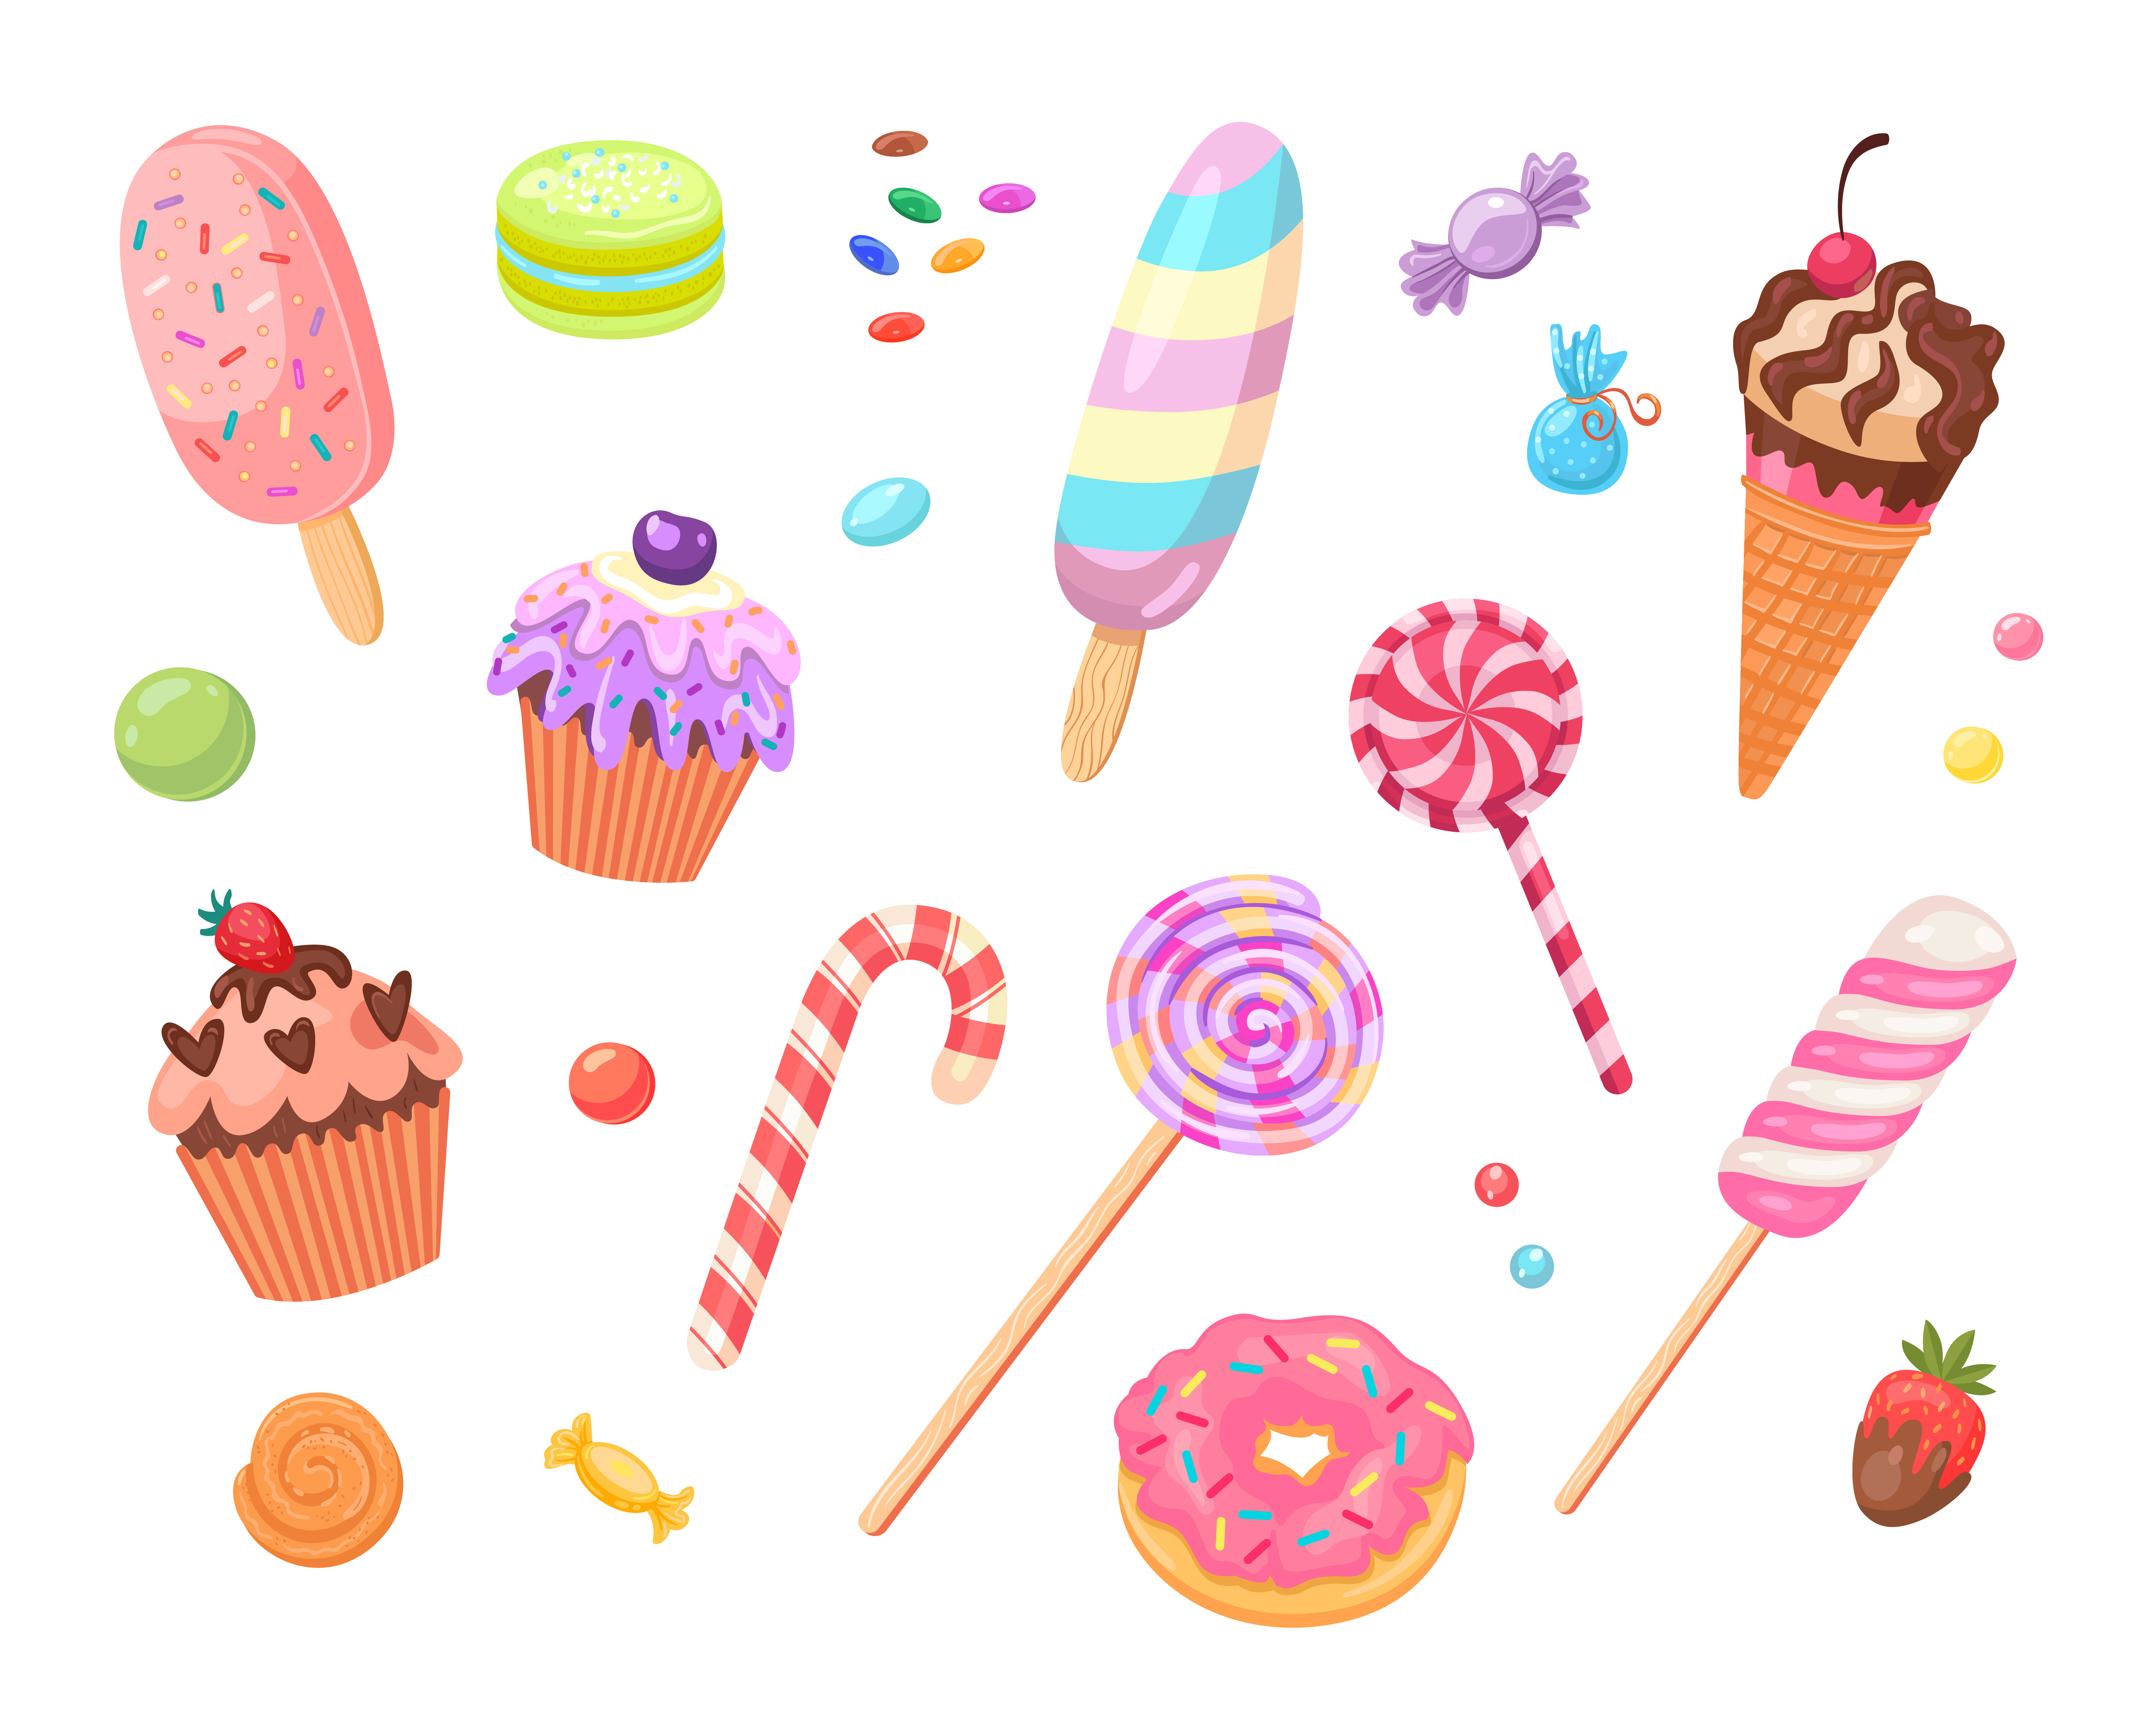
\includegraphics[width=\paperwidth,height=\paperheight]{../images/sweets-cakes-flat-icon-set.jpg}
      }%
  }
  \BgThispage
  
  \begin{center}
    \huge
    Tabuada de Adição
  \end{center}

  \large
  \vspace{40pt}
  \noindent
  Registre o tempo gasto (em minutos):
  \begin{table}[!htpb]
    \begin{tabular}{|c|c|c|c|c|}
      \hline
      
    \begin{tabular}{ccccc}
1 & + & 5 & = & \\
    1 & + & 8 & = & \\
    1 & + & 2 & = & \\
    1 & + & 9 & = & \\
    1 & + & 3 & = & \\
    1 & + & 7 & = & \\
    1 & + & 10 & = & \\
    1 & + & 1 & = & \\
    1 & + & 4 & = & \\
    1 & + & 6 & = &
\end{tabular}&
    \begin{tabular}{ccccc}
2 & + & 3 & = & \\
    2 & + & 10 & = & \\
    2 & + & 7 & = & \\
    2 & + & 2 & = & \\
    2 & + & 1 & = & \\
    2 & + & 8 & = & \\
    2 & + & 6 & = & \\
    2 & + & 5 & = & \\
    2 & + & 9 & = & \\
    2 & + & 4 & = &
\end{tabular}&
    \begin{tabular}{ccccc}
3 & + & 4 & = & \\
    3 & + & 7 & = & \\
    3 & + & 3 & = & \\
    3 & + & 9 & = & \\
    3 & + & 2 & = & \\
    3 & + & 5 & = & \\
    3 & + & 8 & = & \\
    3 & + & 6 & = & \\
    3 & + & 1 & = & \\
    3 & + & 10 & = &
\end{tabular}&
    \begin{tabular}{ccccc}
4 & + & 8 & = & \\
    4 & + & 5 & = & \\
    4 & + & 2 & = & \\
    4 & + & 7 & = & \\
    4 & + & 3 & = & \\
    4 & + & 4 & = & \\
    4 & + & 10 & = & \\
    4 & + & 1 & = & \\
    4 & + & 6 & = & \\
    4 & + & 9 & = &
\end{tabular}&
    \begin{tabular}{ccccc}
5 & + & 7 & = & \\
    5 & + & 10 & = & \\
    5 & + & 9 & = & \\
    5 & + & 2 & = & \\
    5 & + & 8 & = & \\
    5 & + & 1 & = & \\
    5 & + & 5 & = & \\
    5 & + & 6 & = & \\
    5 & + & 3 & = & \\
    5 & + & 4 & = &
\end{tabular}
\\ \hline
    \begin{tabular}{ccccc}
6 & + & 10 & = & \\
    6 & + & 3 & = & \\
    6 & + & 6 & = & \\
    6 & + & 9 & = & \\
    6 & + & 2 & = & \\
    6 & + & 8 & = & \\
    6 & + & 1 & = & \\
    6 & + & 5 & = & \\
    6 & + & 7 & = & \\
    6 & + & 4 & = &
\end{tabular}&
    \begin{tabular}{ccccc}
7 & + & 2 & = & \\
    7 & + & 9 & = & \\
    7 & + & 6 & = & \\
    7 & + & 8 & = & \\
    7 & + & 7 & = & \\
    7 & + & 5 & = & \\
    7 & + & 3 & = & \\
    7 & + & 4 & = & \\
    7 & + & 10 & = & \\
    7 & + & 1 & = &
\end{tabular}&
    \begin{tabular}{ccccc}
8 & + & 5 & = & \\
    8 & + & 9 & = & \\
    8 & + & 10 & = & \\
    8 & + & 6 & = & \\
    8 & + & 2 & = & \\
    8 & + & 8 & = & \\
    8 & + & 7 & = & \\
    8 & + & 4 & = & \\
    8 & + & 1 & = & \\
    8 & + & 3 & = &
\end{tabular}&
    \begin{tabular}{ccccc}
9 & + & 8 & = & \\
    9 & + & 3 & = & \\
    9 & + & 4 & = & \\
    9 & + & 10 & = & \\
    9 & + & 2 & = & \\
    9 & + & 6 & = & \\
    9 & + & 7 & = & \\
    9 & + & 9 & = & \\
    9 & + & 1 & = & \\
    9 & + & 5 & = &
\end{tabular}&
    \begin{tabular}{ccccc}
10 & + & 8 & = & \\
    10 & + & 4 & = & \\
    10 & + & 10 & = & \\
    10 & + & 2 & = & \\
    10 & + & 1 & = & \\
    10 & + & 7 & = & \\
    10 & + & 3 & = & \\
    10 & + & 5 & = & \\
    10 & + & 9 & = & \\
    10 & + & 6 & = &
\end{tabular}
      \\ \hline
    \end{tabular}
  \end{table}
  \vfil
  \begin{flushright}
    \begin{minipage}[b]{6cm}
      A tabuada é o objeto de estudo mais importante na Matemática. É o caminho para se chegar ao universo dos números. (José Carlos dos Santos)
    \end{minipage}
  \end{flushright}

  \newpage
  

  \backgroundsetup{
    scale=1,
    color=black,
    opacity=0.2,
    angle=0,
    contents={%
        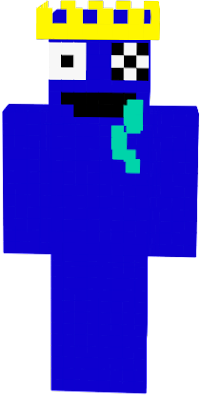
\includegraphics[width=\paperwidth,height=\paperheight]{../images/babao.png}
      }%
  }
  \BgThispage
  
  \begin{center}
    \huge
    Tabuada de Adição
  \end{center}

  \large
  \vspace{40pt}
  \noindent
  Registre o tempo gasto (em minutos):
  \begin{table}[!htpb]
    \begin{tabular}{|c|c|c|c|c|}
      \hline
      
    \begin{tabular}{ccccc}
1 & + & 8 & = & \\
    1 & + & 1 & = & \\
    1 & + & 3 & = & \\
    1 & + & 5 & = & \\
    1 & + & 6 & = & \\
    1 & + & 4 & = & \\
    1 & + & 9 & = & \\
    1 & + & 7 & = & \\
    1 & + & 2 & = & \\
    1 & + & 10 & = &
\end{tabular}&
    \begin{tabular}{ccccc}
2 & + & 2 & = & \\
    2 & + & 8 & = & \\
    2 & + & 1 & = & \\
    2 & + & 3 & = & \\
    2 & + & 6 & = & \\
    2 & + & 7 & = & \\
    2 & + & 4 & = & \\
    2 & + & 5 & = & \\
    2 & + & 10 & = & \\
    2 & + & 9 & = &
\end{tabular}&
    \begin{tabular}{ccccc}
3 & + & 8 & = & \\
    3 & + & 9 & = & \\
    3 & + & 3 & = & \\
    3 & + & 10 & = & \\
    3 & + & 2 & = & \\
    3 & + & 4 & = & \\
    3 & + & 6 & = & \\
    3 & + & 7 & = & \\
    3 & + & 1 & = & \\
    3 & + & 5 & = &
\end{tabular}&
    \begin{tabular}{ccccc}
4 & + & 6 & = & \\
    4 & + & 7 & = & \\
    4 & + & 9 & = & \\
    4 & + & 5 & = & \\
    4 & + & 1 & = & \\
    4 & + & 3 & = & \\
    4 & + & 8 & = & \\
    4 & + & 2 & = & \\
    4 & + & 4 & = & \\
    4 & + & 10 & = &
\end{tabular}&
    \begin{tabular}{ccccc}
5 & + & 3 & = & \\
    5 & + & 5 & = & \\
    5 & + & 8 & = & \\
    5 & + & 10 & = & \\
    5 & + & 4 & = & \\
    5 & + & 2 & = & \\
    5 & + & 9 & = & \\
    5 & + & 6 & = & \\
    5 & + & 1 & = & \\
    5 & + & 7 & = &
\end{tabular}
\\ \hline
    \begin{tabular}{ccccc}
6 & + & 10 & = & \\
    6 & + & 1 & = & \\
    6 & + & 5 & = & \\
    6 & + & 8 & = & \\
    6 & + & 6 & = & \\
    6 & + & 2 & = & \\
    6 & + & 3 & = & \\
    6 & + & 4 & = & \\
    6 & + & 7 & = & \\
    6 & + & 9 & = &
\end{tabular}&
    \begin{tabular}{ccccc}
7 & + & 9 & = & \\
    7 & + & 6 & = & \\
    7 & + & 5 & = & \\
    7 & + & 2 & = & \\
    7 & + & 1 & = & \\
    7 & + & 3 & = & \\
    7 & + & 8 & = & \\
    7 & + & 4 & = & \\
    7 & + & 7 & = & \\
    7 & + & 10 & = &
\end{tabular}&
    \begin{tabular}{ccccc}
8 & + & 2 & = & \\
    8 & + & 8 & = & \\
    8 & + & 10 & = & \\
    8 & + & 7 & = & \\
    8 & + & 6 & = & \\
    8 & + & 5 & = & \\
    8 & + & 9 & = & \\
    8 & + & 3 & = & \\
    8 & + & 4 & = & \\
    8 & + & 1 & = &
\end{tabular}&
    \begin{tabular}{ccccc}
9 & + & 8 & = & \\
    9 & + & 6 & = & \\
    9 & + & 5 & = & \\
    9 & + & 4 & = & \\
    9 & + & 2 & = & \\
    9 & + & 1 & = & \\
    9 & + & 10 & = & \\
    9 & + & 9 & = & \\
    9 & + & 7 & = & \\
    9 & + & 3 & = &
\end{tabular}&
    \begin{tabular}{ccccc}
10 & + & 8 & = & \\
    10 & + & 9 & = & \\
    10 & + & 1 & = & \\
    10 & + & 10 & = & \\
    10 & + & 2 & = & \\
    10 & + & 6 & = & \\
    10 & + & 4 & = & \\
    10 & + & 3 & = & \\
    10 & + & 7 & = & \\
    10 & + & 5 & = &
\end{tabular}
      \\ \hline
    \end{tabular}
  \end{table}
  \vfil
  \begin{flushright}
    \begin{minipage}[b]{6cm}
      A tabuada é o objeto de estudo mais importante na Matemática. É o caminho para se chegar ao universo dos números. (José Carlos dos Santos)
    \end{minipage}
  \end{flushright}

  \newpage
  

  \backgroundsetup{
    scale=1,
    color=black,
    opacity=0.2,
    angle=0,
    contents={%
        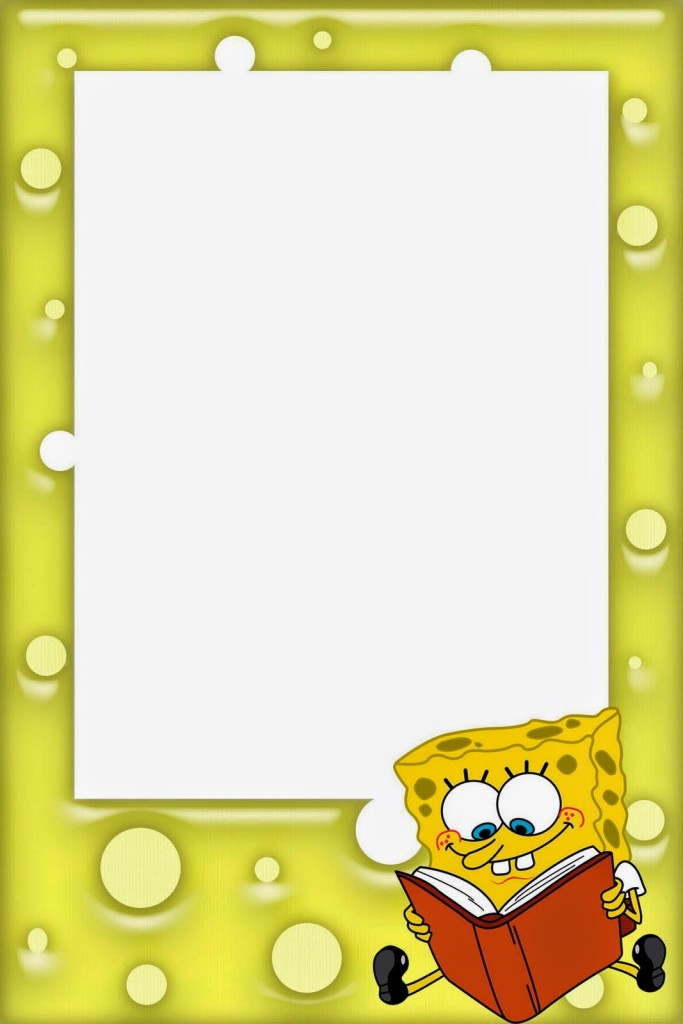
\includegraphics[width=\paperwidth,height=\paperheight]{../images/Bob-Esponja-estudando.jpg}
      }%
  }
  \BgThispage
  
  \begin{center}
    \huge
    Tabuada de Adição
  \end{center}

  \large
  \vspace{40pt}
  \noindent
  Registre o tempo gasto (em minutos):
  \begin{table}[!htpb]
    \begin{tabular}{|c|c|c|c|c|}
      \hline
      
    \begin{tabular}{ccccc}
1 & + & 7 & = & \\
    1 & + & 2 & = & \\
    1 & + & 6 & = & \\
    1 & + & 9 & = & \\
    1 & + & 1 & = & \\
    1 & + & 3 & = & \\
    1 & + & 4 & = & \\
    1 & + & 8 & = & \\
    1 & + & 10 & = & \\
    1 & + & 5 & = &
\end{tabular}&
    \begin{tabular}{ccccc}
2 & + & 8 & = & \\
    2 & + & 4 & = & \\
    2 & + & 5 & = & \\
    2 & + & 9 & = & \\
    2 & + & 3 & = & \\
    2 & + & 1 & = & \\
    2 & + & 10 & = & \\
    2 & + & 7 & = & \\
    2 & + & 6 & = & \\
    2 & + & 2 & = &
\end{tabular}&
    \begin{tabular}{ccccc}
3 & + & 6 & = & \\
    3 & + & 1 & = & \\
    3 & + & 4 & = & \\
    3 & + & 7 & = & \\
    3 & + & 5 & = & \\
    3 & + & 8 & = & \\
    3 & + & 3 & = & \\
    3 & + & 2 & = & \\
    3 & + & 10 & = & \\
    3 & + & 9 & = &
\end{tabular}&
    \begin{tabular}{ccccc}
4 & + & 4 & = & \\
    4 & + & 2 & = & \\
    4 & + & 6 & = & \\
    4 & + & 3 & = & \\
    4 & + & 1 & = & \\
    4 & + & 9 & = & \\
    4 & + & 10 & = & \\
    4 & + & 7 & = & \\
    4 & + & 5 & = & \\
    4 & + & 8 & = &
\end{tabular}&
    \begin{tabular}{ccccc}
5 & + & 10 & = & \\
    5 & + & 4 & = & \\
    5 & + & 3 & = & \\
    5 & + & 8 & = & \\
    5 & + & 1 & = & \\
    5 & + & 9 & = & \\
    5 & + & 6 & = & \\
    5 & + & 5 & = & \\
    5 & + & 2 & = & \\
    5 & + & 7 & = &
\end{tabular}
\\ \hline
    \begin{tabular}{ccccc}
6 & + & 9 & = & \\
    6 & + & 6 & = & \\
    6 & + & 8 & = & \\
    6 & + & 7 & = & \\
    6 & + & 3 & = & \\
    6 & + & 2 & = & \\
    6 & + & 10 & = & \\
    6 & + & 4 & = & \\
    6 & + & 1 & = & \\
    6 & + & 5 & = &
\end{tabular}&
    \begin{tabular}{ccccc}
7 & + & 3 & = & \\
    7 & + & 2 & = & \\
    7 & + & 10 & = & \\
    7 & + & 4 & = & \\
    7 & + & 1 & = & \\
    7 & + & 6 & = & \\
    7 & + & 8 & = & \\
    7 & + & 5 & = & \\
    7 & + & 7 & = & \\
    7 & + & 9 & = &
\end{tabular}&
    \begin{tabular}{ccccc}
8 & + & 9 & = & \\
    8 & + & 6 & = & \\
    8 & + & 10 & = & \\
    8 & + & 4 & = & \\
    8 & + & 5 & = & \\
    8 & + & 3 & = & \\
    8 & + & 7 & = & \\
    8 & + & 1 & = & \\
    8 & + & 2 & = & \\
    8 & + & 8 & = &
\end{tabular}&
    \begin{tabular}{ccccc}
9 & + & 10 & = & \\
    9 & + & 2 & = & \\
    9 & + & 7 & = & \\
    9 & + & 9 & = & \\
    9 & + & 5 & = & \\
    9 & + & 8 & = & \\
    9 & + & 3 & = & \\
    9 & + & 4 & = & \\
    9 & + & 1 & = & \\
    9 & + & 6 & = &
\end{tabular}&
    \begin{tabular}{ccccc}
10 & + & 3 & = & \\
    10 & + & 6 & = & \\
    10 & + & 4 & = & \\
    10 & + & 10 & = & \\
    10 & + & 1 & = & \\
    10 & + & 5 & = & \\
    10 & + & 8 & = & \\
    10 & + & 2 & = & \\
    10 & + & 9 & = & \\
    10 & + & 7 & = &
\end{tabular}
      \\ \hline
    \end{tabular}
  \end{table}
  \vfil
  \begin{flushright}
    \begin{minipage}[b]{6cm}
      A tabuada é o objeto de estudo mais importante na Matemática. É o caminho para se chegar ao universo dos números. (José Carlos dos Santos)
    \end{minipage}
  \end{flushright}

  \newpage
  

  \backgroundsetup{
    scale=1,
    color=black,
    opacity=0.2,
    angle=0,
    contents={%
        \includegraphics[width=\paperwidth,height=\paperheight]{../images/cute-galaxy-blue-frame-white-background-kids.jpg}
      }%
  }
  \BgThispage
  
  \begin{center}
    \huge
    Tabuada de Adição
  \end{center}

  \large
  \vspace{40pt}
  \noindent
  Registre o tempo gasto (em minutos):
  \begin{table}[!htpb]
    \begin{tabular}{|c|c|c|c|c|}
      \hline
      
    \begin{tabular}{ccccc}
1 & + & 2 & = & \\
    1 & + & 5 & = & \\
    1 & + & 3 & = & \\
    1 & + & 4 & = & \\
    1 & + & 1 & = & \\
    1 & + & 6 & = & \\
    1 & + & 10 & = & \\
    1 & + & 8 & = & \\
    1 & + & 7 & = & \\
    1 & + & 9 & = &
\end{tabular}&
    \begin{tabular}{ccccc}
2 & + & 6 & = & \\
    2 & + & 1 & = & \\
    2 & + & 8 & = & \\
    2 & + & 9 & = & \\
    2 & + & 4 & = & \\
    2 & + & 5 & = & \\
    2 & + & 10 & = & \\
    2 & + & 2 & = & \\
    2 & + & 3 & = & \\
    2 & + & 7 & = &
\end{tabular}&
    \begin{tabular}{ccccc}
3 & + & 10 & = & \\
    3 & + & 9 & = & \\
    3 & + & 4 & = & \\
    3 & + & 7 & = & \\
    3 & + & 3 & = & \\
    3 & + & 6 & = & \\
    3 & + & 2 & = & \\
    3 & + & 1 & = & \\
    3 & + & 8 & = & \\
    3 & + & 5 & = &
\end{tabular}&
    \begin{tabular}{ccccc}
4 & + & 1 & = & \\
    4 & + & 4 & = & \\
    4 & + & 6 & = & \\
    4 & + & 10 & = & \\
    4 & + & 2 & = & \\
    4 & + & 8 & = & \\
    4 & + & 9 & = & \\
    4 & + & 7 & = & \\
    4 & + & 3 & = & \\
    4 & + & 5 & = &
\end{tabular}&
    \begin{tabular}{ccccc}
5 & + & 4 & = & \\
    5 & + & 5 & = & \\
    5 & + & 9 & = & \\
    5 & + & 10 & = & \\
    5 & + & 1 & = & \\
    5 & + & 7 & = & \\
    5 & + & 6 & = & \\
    5 & + & 3 & = & \\
    5 & + & 8 & = & \\
    5 & + & 2 & = &
\end{tabular}
\\ \hline
    \begin{tabular}{ccccc}
6 & + & 8 & = & \\
    6 & + & 10 & = & \\
    6 & + & 5 & = & \\
    6 & + & 9 & = & \\
    6 & + & 7 & = & \\
    6 & + & 1 & = & \\
    6 & + & 3 & = & \\
    6 & + & 6 & = & \\
    6 & + & 2 & = & \\
    6 & + & 4 & = &
\end{tabular}&
    \begin{tabular}{ccccc}
7 & + & 6 & = & \\
    7 & + & 5 & = & \\
    7 & + & 7 & = & \\
    7 & + & 2 & = & \\
    7 & + & 8 & = & \\
    7 & + & 1 & = & \\
    7 & + & 4 & = & \\
    7 & + & 9 & = & \\
    7 & + & 3 & = & \\
    7 & + & 10 & = &
\end{tabular}&
    \begin{tabular}{ccccc}
8 & + & 4 & = & \\
    8 & + & 10 & = & \\
    8 & + & 3 & = & \\
    8 & + & 7 & = & \\
    8 & + & 9 & = & \\
    8 & + & 8 & = & \\
    8 & + & 6 & = & \\
    8 & + & 5 & = & \\
    8 & + & 2 & = & \\
    8 & + & 1 & = &
\end{tabular}&
    \begin{tabular}{ccccc}
9 & + & 7 & = & \\
    9 & + & 3 & = & \\
    9 & + & 10 & = & \\
    9 & + & 9 & = & \\
    9 & + & 6 & = & \\
    9 & + & 2 & = & \\
    9 & + & 4 & = & \\
    9 & + & 8 & = & \\
    9 & + & 5 & = & \\
    9 & + & 1 & = &
\end{tabular}&
    \begin{tabular}{ccccc}
10 & + & 10 & = & \\
    10 & + & 1 & = & \\
    10 & + & 5 & = & \\
    10 & + & 4 & = & \\
    10 & + & 7 & = & \\
    10 & + & 9 & = & \\
    10 & + & 2 & = & \\
    10 & + & 8 & = & \\
    10 & + & 3 & = & \\
    10 & + & 6 & = &
\end{tabular}
      \\ \hline
    \end{tabular}
  \end{table}
  \vfil
  \begin{flushright}
    \begin{minipage}[b]{6cm}
      A tabuada é o objeto de estudo mais importante na Matemática. É o caminho para se chegar ao universo dos números. (José Carlos dos Santos)
    \end{minipage}
  \end{flushright}

  \newpage
  

  \backgroundsetup{
    scale=1,
    color=black,
    opacity=0.2,
    angle=0,
    contents={%
        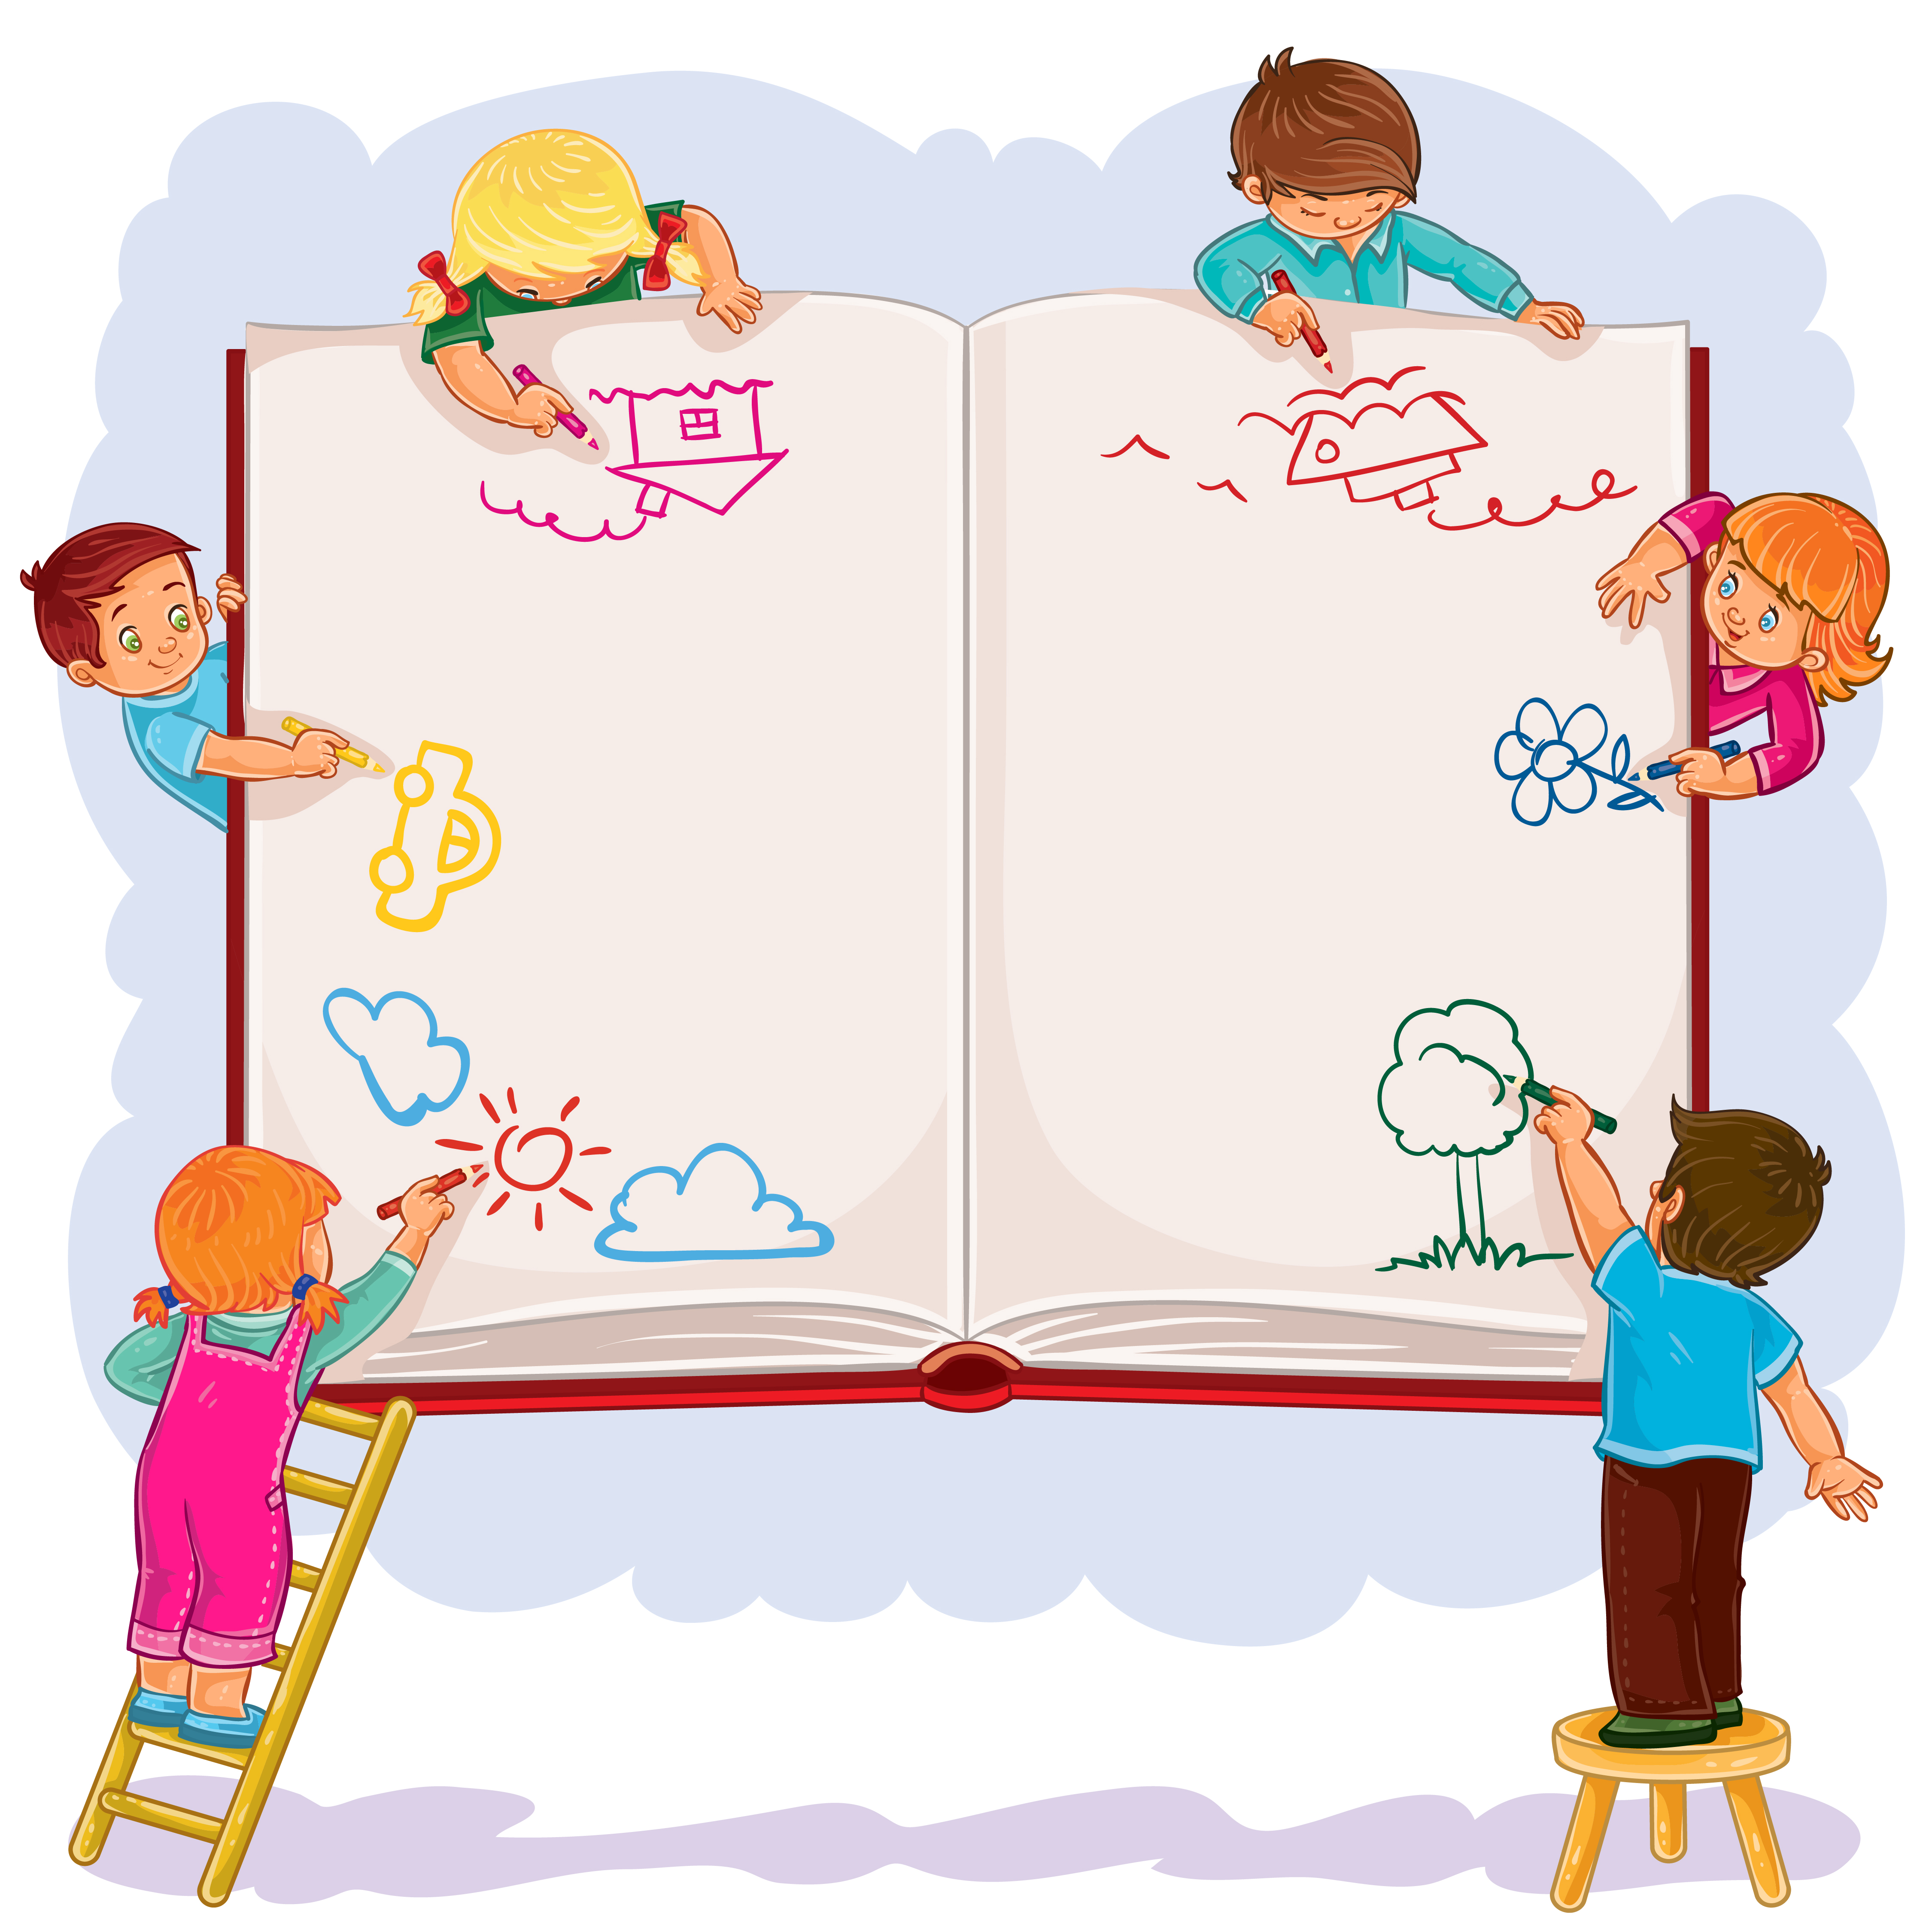
\includegraphics[width=\paperwidth,height=\paperheight]{../images/happy-children-together-draw-large-sheet-book.jpg}
      }%
  }
  \BgThispage
  
  \begin{center}
    \huge
    Tabuada de Adição
  \end{center}

  \large
  \vspace{40pt}
  \noindent
  Registre o tempo gasto (em minutos):
  \begin{table}[!htpb]
    \begin{tabular}{|c|c|c|c|c|}
      \hline
      
    \begin{tabular}{ccccc}
1 & + & 9 & = & \\
    1 & + & 10 & = & \\
    1 & + & 3 & = & \\
    1 & + & 2 & = & \\
    1 & + & 4 & = & \\
    1 & + & 8 & = & \\
    1 & + & 1 & = & \\
    1 & + & 5 & = & \\
    1 & + & 6 & = & \\
    1 & + & 7 & = &
\end{tabular}&
    \begin{tabular}{ccccc}
2 & + & 7 & = & \\
    2 & + & 5 & = & \\
    2 & + & 6 & = & \\
    2 & + & 9 & = & \\
    2 & + & 3 & = & \\
    2 & + & 10 & = & \\
    2 & + & 1 & = & \\
    2 & + & 8 & = & \\
    2 & + & 4 & = & \\
    2 & + & 2 & = &
\end{tabular}&
    \begin{tabular}{ccccc}
3 & + & 2 & = & \\
    3 & + & 6 & = & \\
    3 & + & 5 & = & \\
    3 & + & 8 & = & \\
    3 & + & 9 & = & \\
    3 & + & 7 & = & \\
    3 & + & 10 & = & \\
    3 & + & 4 & = & \\
    3 & + & 1 & = & \\
    3 & + & 3 & = &
\end{tabular}&
    \begin{tabular}{ccccc}
4 & + & 10 & = & \\
    4 & + & 1 & = & \\
    4 & + & 3 & = & \\
    4 & + & 5 & = & \\
    4 & + & 4 & = & \\
    4 & + & 7 & = & \\
    4 & + & 6 & = & \\
    4 & + & 2 & = & \\
    4 & + & 9 & = & \\
    4 & + & 8 & = &
\end{tabular}&
    \begin{tabular}{ccccc}
5 & + & 7 & = & \\
    5 & + & 8 & = & \\
    5 & + & 9 & = & \\
    5 & + & 1 & = & \\
    5 & + & 6 & = & \\
    5 & + & 10 & = & \\
    5 & + & 5 & = & \\
    5 & + & 2 & = & \\
    5 & + & 3 & = & \\
    5 & + & 4 & = &
\end{tabular}
\\ \hline
    \begin{tabular}{ccccc}
6 & + & 9 & = & \\
    6 & + & 6 & = & \\
    6 & + & 8 & = & \\
    6 & + & 1 & = & \\
    6 & + & 2 & = & \\
    6 & + & 7 & = & \\
    6 & + & 4 & = & \\
    6 & + & 5 & = & \\
    6 & + & 3 & = & \\
    6 & + & 10 & = &
\end{tabular}&
    \begin{tabular}{ccccc}
7 & + & 4 & = & \\
    7 & + & 7 & = & \\
    7 & + & 10 & = & \\
    7 & + & 8 & = & \\
    7 & + & 5 & = & \\
    7 & + & 1 & = & \\
    7 & + & 6 & = & \\
    7 & + & 2 & = & \\
    7 & + & 3 & = & \\
    7 & + & 9 & = &
\end{tabular}&
    \begin{tabular}{ccccc}
8 & + & 7 & = & \\
    8 & + & 6 & = & \\
    8 & + & 8 & = & \\
    8 & + & 4 & = & \\
    8 & + & 2 & = & \\
    8 & + & 5 & = & \\
    8 & + & 9 & = & \\
    8 & + & 1 & = & \\
    8 & + & 10 & = & \\
    8 & + & 3 & = &
\end{tabular}&
    \begin{tabular}{ccccc}
9 & + & 7 & = & \\
    9 & + & 1 & = & \\
    9 & + & 9 & = & \\
    9 & + & 2 & = & \\
    9 & + & 5 & = & \\
    9 & + & 8 & = & \\
    9 & + & 3 & = & \\
    9 & + & 4 & = & \\
    9 & + & 6 & = & \\
    9 & + & 10 & = &
\end{tabular}&
    \begin{tabular}{ccccc}
10 & + & 1 & = & \\
    10 & + & 4 & = & \\
    10 & + & 7 & = & \\
    10 & + & 10 & = & \\
    10 & + & 8 & = & \\
    10 & + & 3 & = & \\
    10 & + & 9 & = & \\
    10 & + & 2 & = & \\
    10 & + & 5 & = & \\
    10 & + & 6 & = &
\end{tabular}
      \\ \hline
    \end{tabular}
  \end{table}
  \vfil
  \begin{flushright}
    \begin{minipage}[b]{6cm}
      A tabuada é o objeto de estudo mais importante na Matemática. É o caminho para se chegar ao universo dos números. (José Carlos dos Santos)
    \end{minipage}
  \end{flushright}

  \newpage
  
    \end{document}
  